% Ensayos actualizados: cuatro corridas del banco de medio ciclo.
\clearpage
\section{Pruebas de medio ciclo con CODESYS manual}
\label{sec:ensayo_codesys_manual}
\subsection{Objetivo y condiciones comunes}
Se compararon los autómatas supervisor y de seguridad programados manualmente en CODESYS mediante SFC y los autómatas en texto estructurado obtenidos mediante generación automática de código para PLC de Simulink. La planta, sensores, reguladores, visualización y HMI permanecieron en Simulink, conectados al PLC por OPC UA. Los términos manual y automático identifican la implementación de los autómatas; ambas maniobras combinan conducción manual y traslado automático.

Las cuatro pruebas comparten perfil físico, masas, ganancias, condiciones iniciales y operador. Antes de cada corrida se realizó Reset en caliente y se puso el PLC en RUN. Se precargaron las 33 alturas reales de la escena, con perfil válido y barrido no completado. El ensayo comienza directamente con la toma en el muelle y termina al entregar o al detenerse por el criterio establecido; no incluye barrido LiDAR, retorno vacío ni segunda toma.

\begin{table}[!htbp]\centering\small
\caption{Condiciones comunes del banco actualizado.}\label{tab:condiciones_medio_codesys}
\begin{tabular}{L{.31\textwidth}L{.61\textwidth}}\toprule
Condición & Configuración\\\midrule
Inicio y destino & $x=-26.34~\mathrm{m}$, altura $25~\mathrm{m}$, reposo; retiro del slot 2 y destino slot 22, centro $22.46~\mathrm{m}$.\\
Masa suspendida & Spreader: $15\,000~\mathrm{kg}$; contenedor: $36\,863~\mathrm{kg}$; conjunto cargado: $51\,863~\mathrm{kg}$.\\
Perfil & 33 alturas físicas; máximo inicial $18.85~\mathrm{m}$; contenedor de altura $2.59~\mathrm{m}$.\\
Control & Reguladores de carro e izaje comunes; observadores discretizados por Tustin; rampa de habilitación antisway de $2~\mathrm{s}$ y límite de variación de su término anticipativo de $0.25~\mathrm{m/s^2}$.\\
Variante & Ganancia cero o uno sobre la contribución antisway antes de sumarla al comando; cálculo interno conservado.\\
Tiempos & Control: $1~\mathrm{ms}$; actualización de autómatas por trama simulada de $20~\mathrm{ms}$; operador y rejilla de análisis: $40~\mathrm{ms}$.\\
Vigilancia & Latido de enlace independiente en tiempo real; timeout de comunicación de $3~\mathrm{s}$. La sincronización de las máquinas de estados usa el tiempo simulado.\\
Finalización & Sin antisway: límite solicitado de $180~\mathrm{s}$. Con antisway: continuar sin fallas hasta entrega o hasta diagnóstico de bloqueo.\\\bottomrule
\end{tabular}\end{table}

La adaptación del banco separa el reloj de la maniobra simulada de la vigilancia real de comunicaciones. Permite reproducir la secuencia aunque la visualización y el registro ralenticen Simulink. No constituye una validación de ejecución en tiempo real sobre una máquina física. Los límites, ganancias y criterios de descarga no se relajaron para obtener entregas.

\subsection{Procedimiento y comprobación de entrega}
El operador solicita START, entra a manual, aproxima y desciende hasta contacto en el origen, cierra twistlocks, confirma toma y selecciona destino. Eleva manualmente hasta la altura local segura más $1~\mathrm{m}$ y solicita automático después de esperar al menos $2~\mathrm{s}$ y alcanzar $|v_y|<0.03~\mathrm{m/s}$. Cerca del barco solicita manual sólo si el error horizontal es menor que $0.5~\mathrm{m}$, $|v_x|<0.25~\mathrm{m/s}$ y la altura no supera la consigna automática más $0.25~\mathrm{m}$. Después desciende hasta apoyo, abre twistlocks y comprueba la descarga física antes de STOP.

La compuerta de descenso automático exige simultáneamente error horizontal no mayor que $0.08~\mathrm{m}$, velocidad horizontal no mayor que $0.06~\mathrm{m/s}$, $|\theta|\leq0.005~\mathrm{rad}$ y $|\omega|\leq0.012~\mathrm{rad/s}$. Llegar horizontalmente no equivale a completar el descenso. La entrega se confirma por la masa física final de $15\,000~\mathrm{kg}$ y el incremento de $2.59~\mathrm{m}$ en el perfil del destino, además del retiro en el origen. Una indicación de carga vacía del PLC, por sí sola, no confirma la transferencia física.

\subsection{CODESYS manual sin antisway: traslado y espera sin entrega}
START se solicitó a $3.24~\mathrm{s}$, el modo manual se observó a $3.76~\mathrm{s}$ y el cierre de twistlocks se solicitó a $46.64~\mathrm{s}$. La masa cargada se confirmó a $49.52~\mathrm{s}$ y el despegue físico a $50.00~\mathrm{s}$. El operador solicitó automático a $75.32~\mathrm{s}$ y lo observó a $75.44~\mathrm{s}$; la llegada horizontal se registró a $105.68~\mathrm{s}$. No hubo transferencia a manual en destino ni entrega.

La prueba se detuvo a $187.20~\mathrm{s}$ con el contenedor retenido. El límite de tres minutos fue solicitado cuando la simulación ya había superado ese instante; por ello se conserva el tiempo real de parada de la corrida y no se recorta a $180~\mathrm{s}$. Es una prueba válida de comportamiento sin antisway, con medio ciclo incompleto.

Las posiciones muestran la toma, elevación y cruce hacia el barco, seguido de permanencia en altura. Las velocidades disminuyen cerca del destino, mientras las aceleraciones conservan los transitorios de contacto y cambio de movimiento. Las referencias y señales del controlador tienen cobertura hasta $130.72~\mathrm{s}$; muchas señales físicas hasta $177.305~\mathrm{s}$. La telemetría del operador conserva posiciones y modo hasta $187.20~\mathrm{s}$. Las curvas nativas se interrumpen al finalizar su registro: los espacios restantes no representan valores nulos ni reposo demostrado.

\begin{figure}[!htbp]
\centering
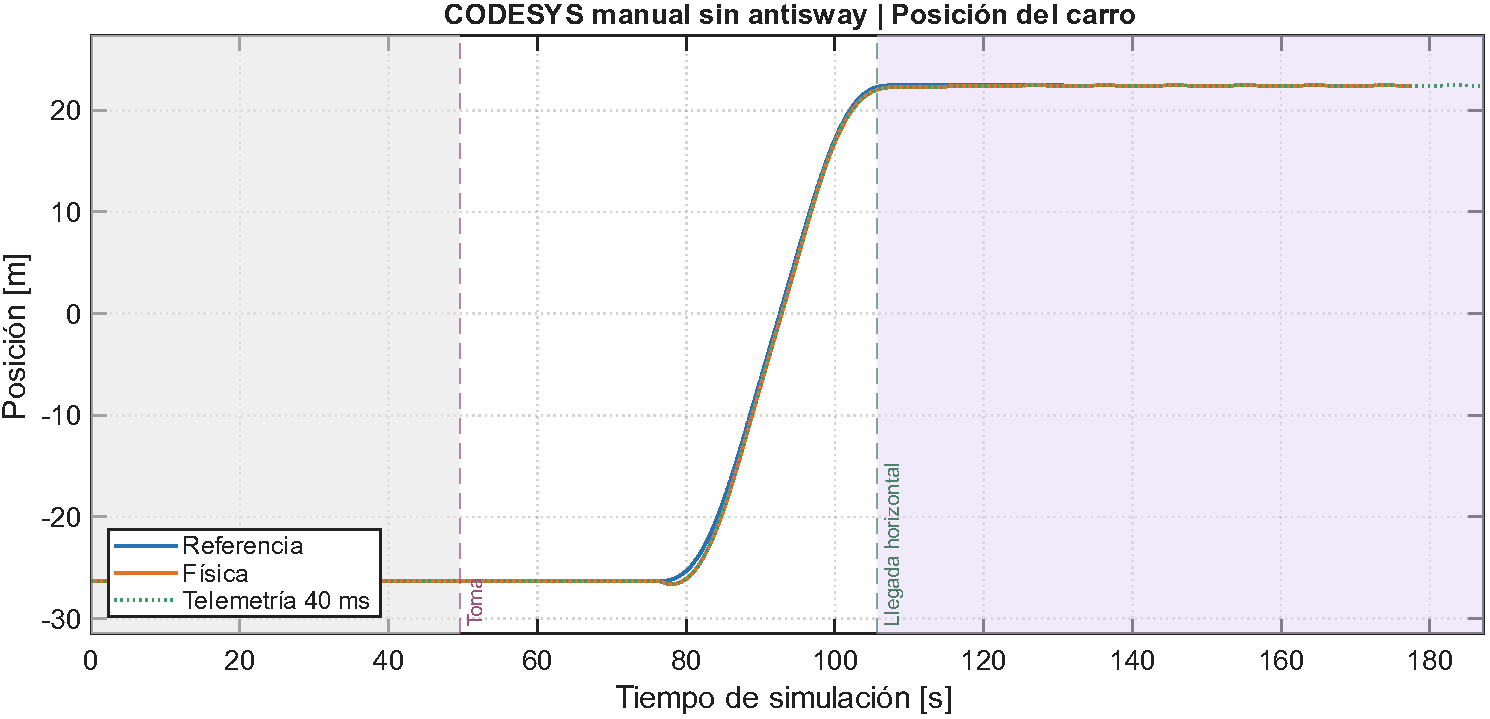
\includegraphics[width=0.98\textwidth]{graficas_individuales/manual_sin_x.pdf}
\caption{CODESYS manual sin antisway: Posición del carro: referencia y evolución física. La telemetría prolonga las posiciones hasta la parada; las referencias terminan en su última muestra.}\label{fig:individual_manual_sin_x}
\end{figure}

\begin{figure}[!htbp]
\centering
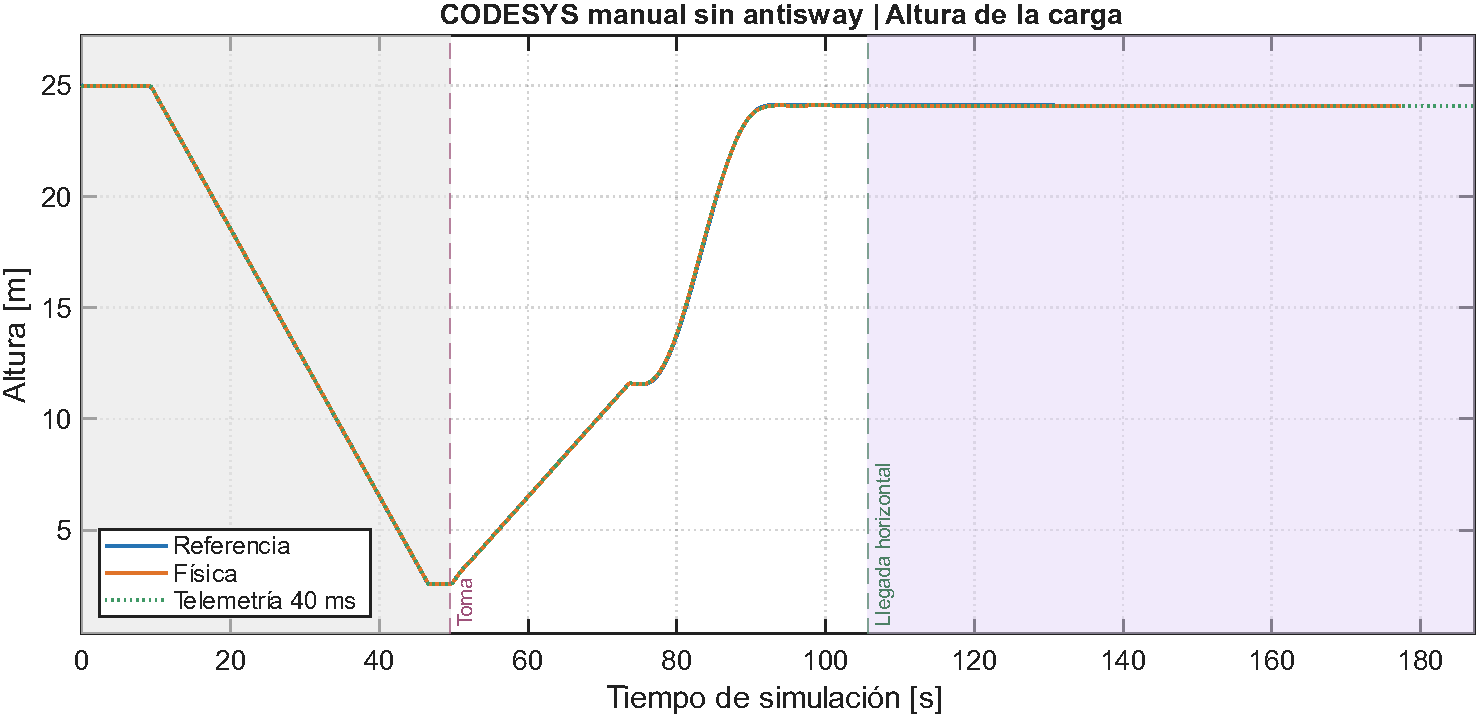
\includegraphics[width=0.98\textwidth]{graficas_individuales/manual_sin_y.pdf}
\caption{CODESYS manual sin antisway: Altura de la carga: referencia y evolución física. La telemetría prolonga las posiciones hasta la parada; las referencias terminan en su última muestra.}\label{fig:individual_manual_sin_y}
\end{figure}

\begin{figure}[!htbp]
\centering
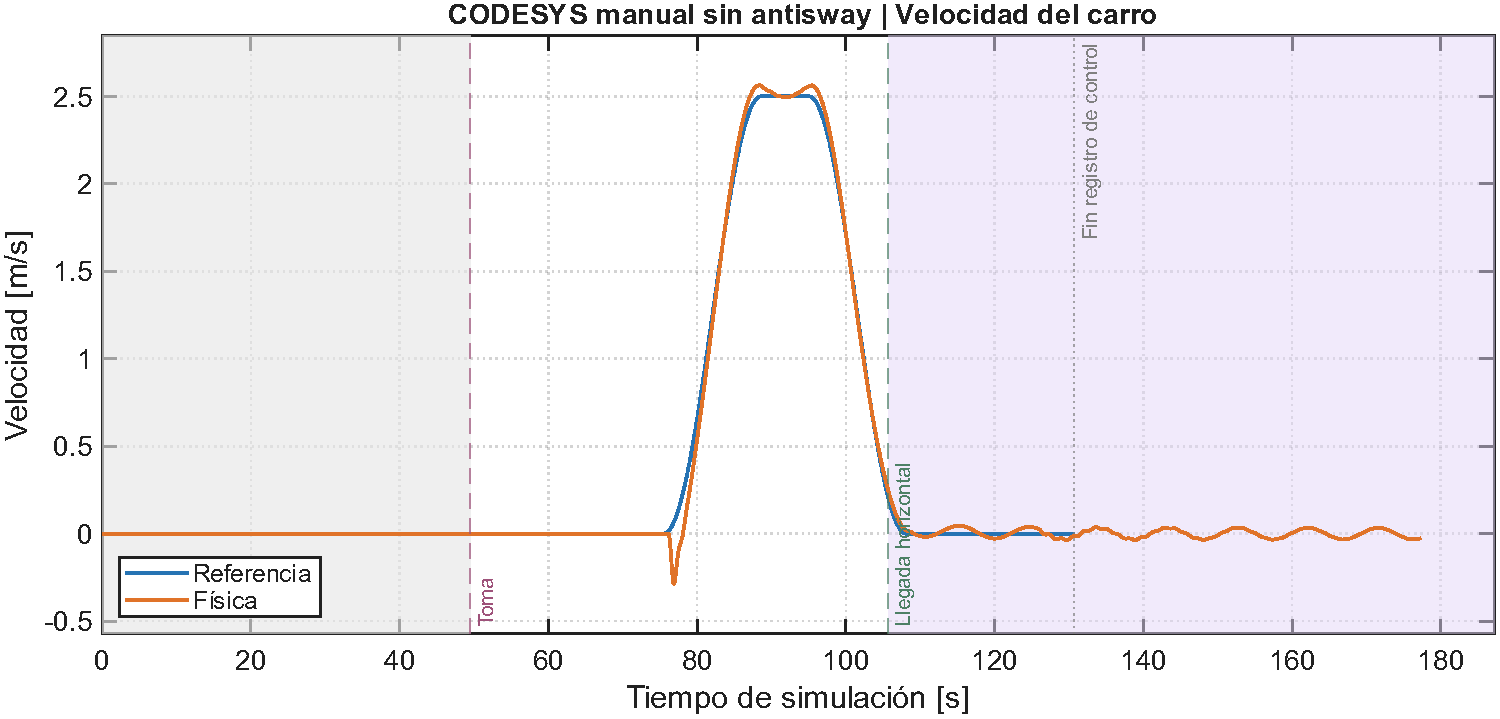
\includegraphics[width=0.98\textwidth]{graficas_individuales/manual_sin_vx.pdf}
\caption{CODESYS manual sin antisway: Velocidad del carro: referencia y señal física. Se respeta la cobertura parcial de las señales y no se extrapolan datos faltantes.}\label{fig:individual_manual_sin_vx}
\end{figure}

\begin{figure}[!htbp]
\centering
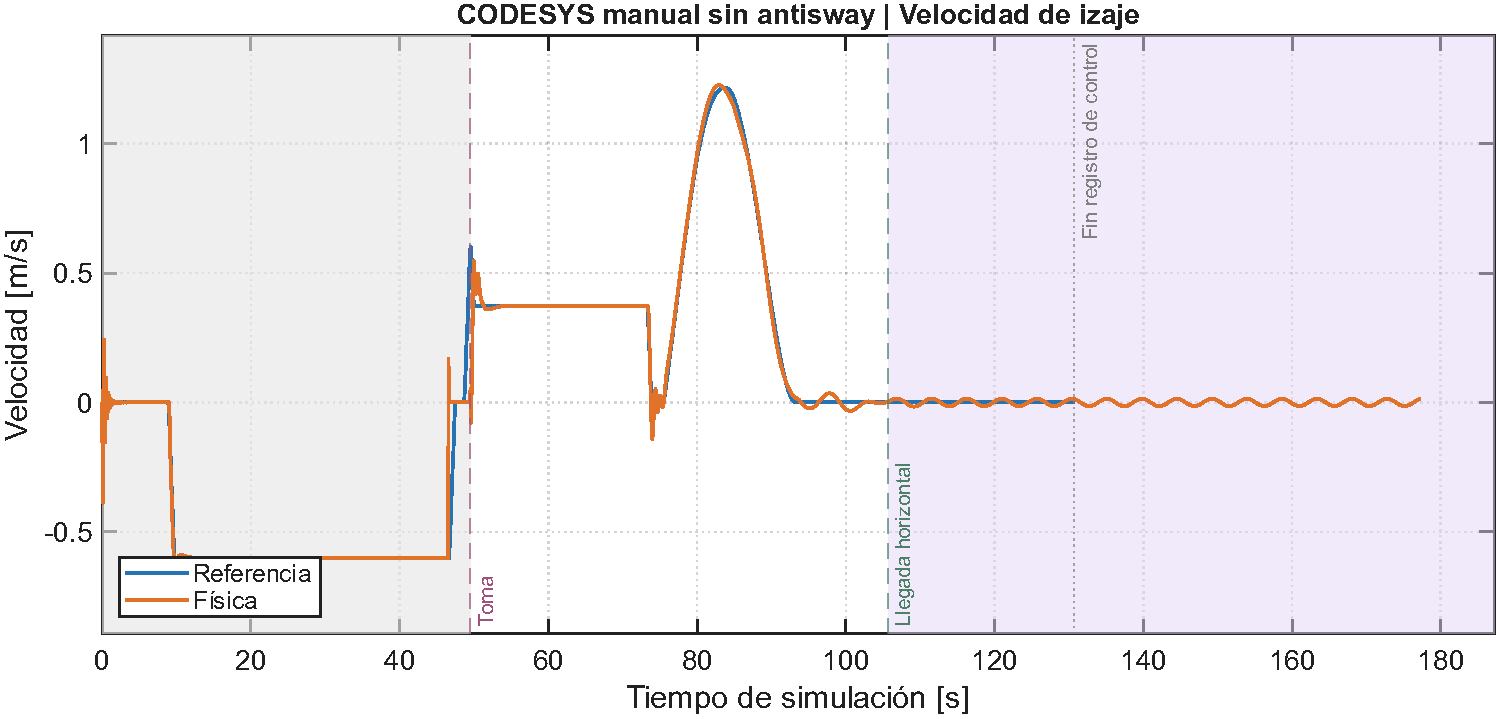
\includegraphics[width=0.98\textwidth]{graficas_individuales/manual_sin_vy.pdf}
\caption{CODESYS manual sin antisway: Velocidad de izaje: referencia y señal física. Se respeta la cobertura parcial de las señales y no se extrapolan datos faltantes.}\label{fig:individual_manual_sin_vy}
\end{figure}

\begin{figure}[!htbp]
\centering
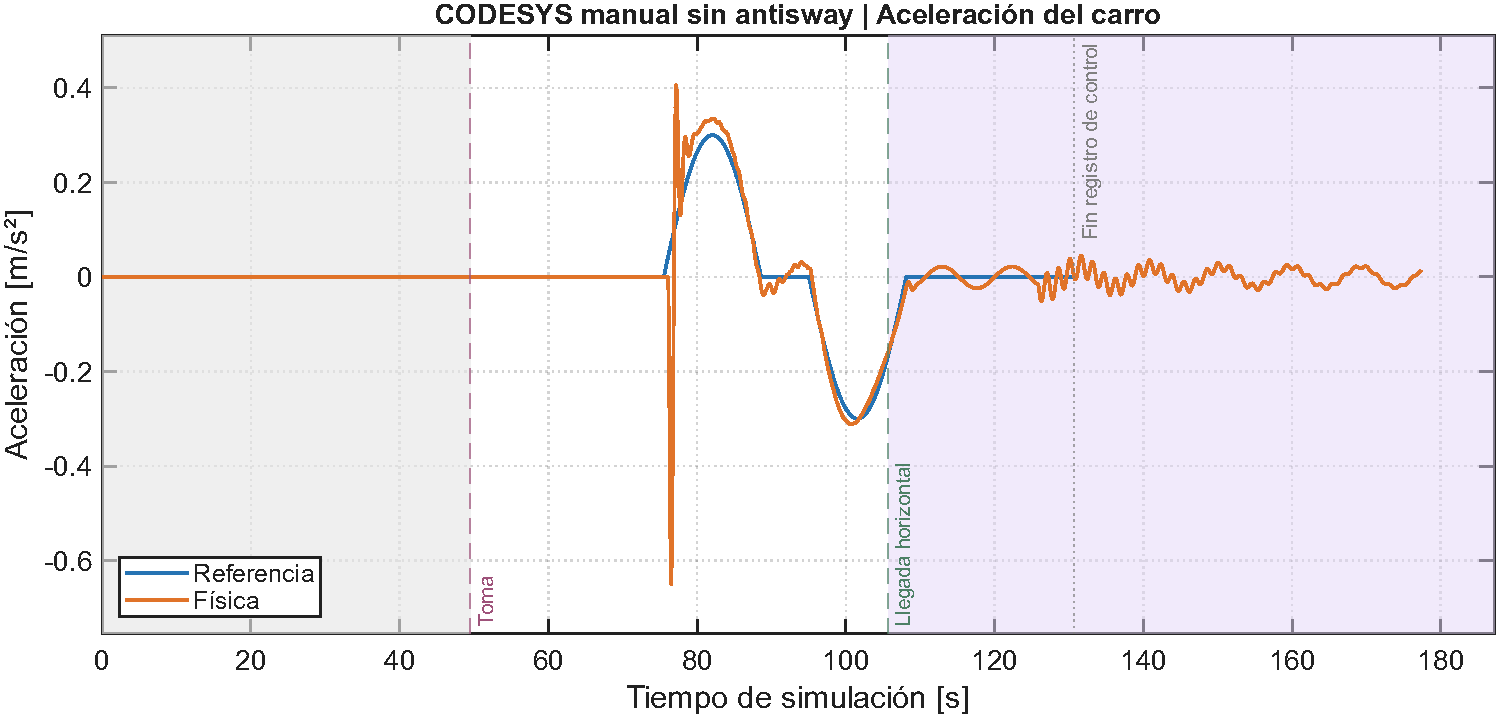
\includegraphics[width=0.98\textwidth]{graficas_individuales/manual_sin_ax.pdf}
\caption{CODESYS manual sin antisway: Aceleración del carro: referencia y señal física. Se respeta la cobertura parcial de las señales y no se extrapolan datos faltantes.}\label{fig:individual_manual_sin_ax}
\end{figure}

\begin{figure}[!htbp]
\centering
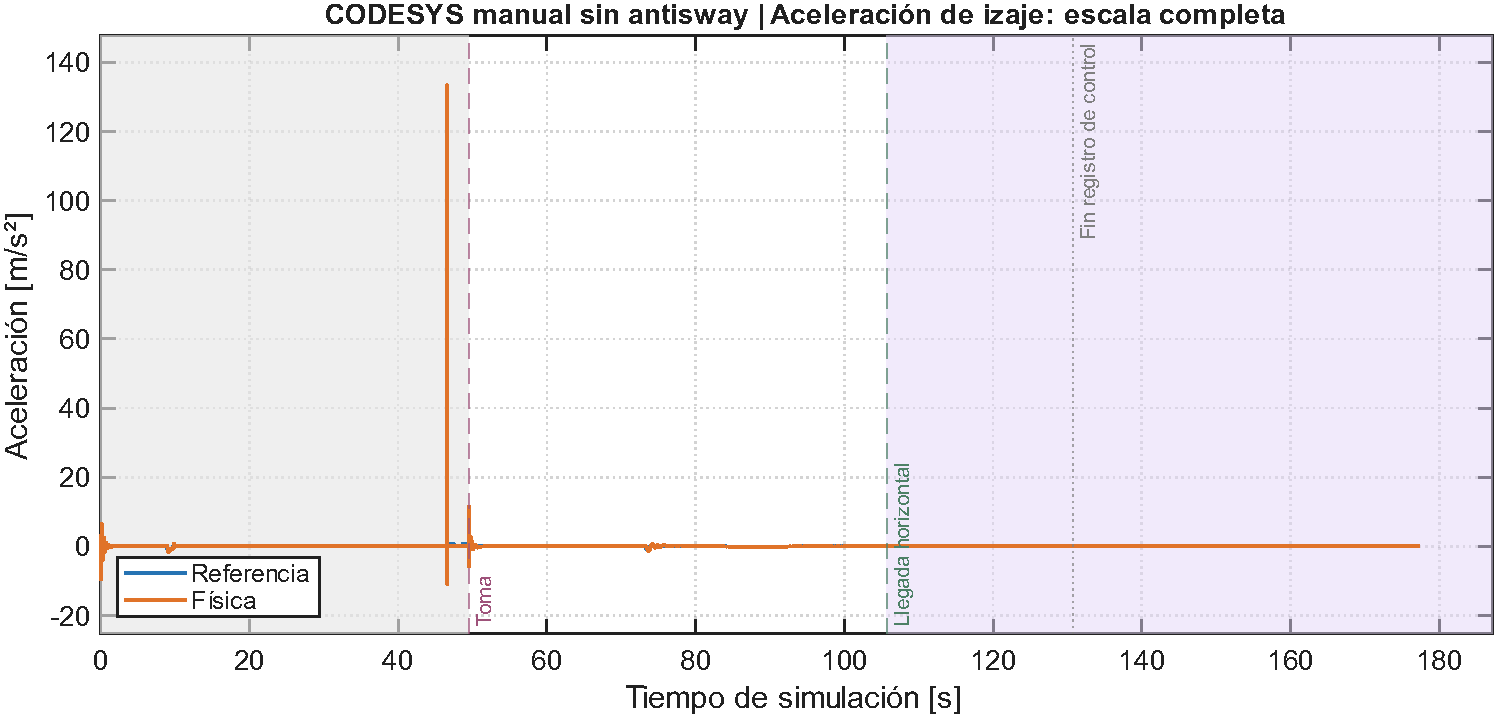
\includegraphics[width=0.98\textwidth]{graficas_individuales/manual_sin_ay.pdf}
\caption{CODESYS manual sin antisway: Aceleración de izaje en escala completa; se conservan los picos de contacto y arranque. Se respeta la cobertura parcial de las señales y no se extrapolan datos faltantes.}\label{fig:individual_manual_sin_ay}
\end{figure}

\begin{figure}[!htbp]
\centering
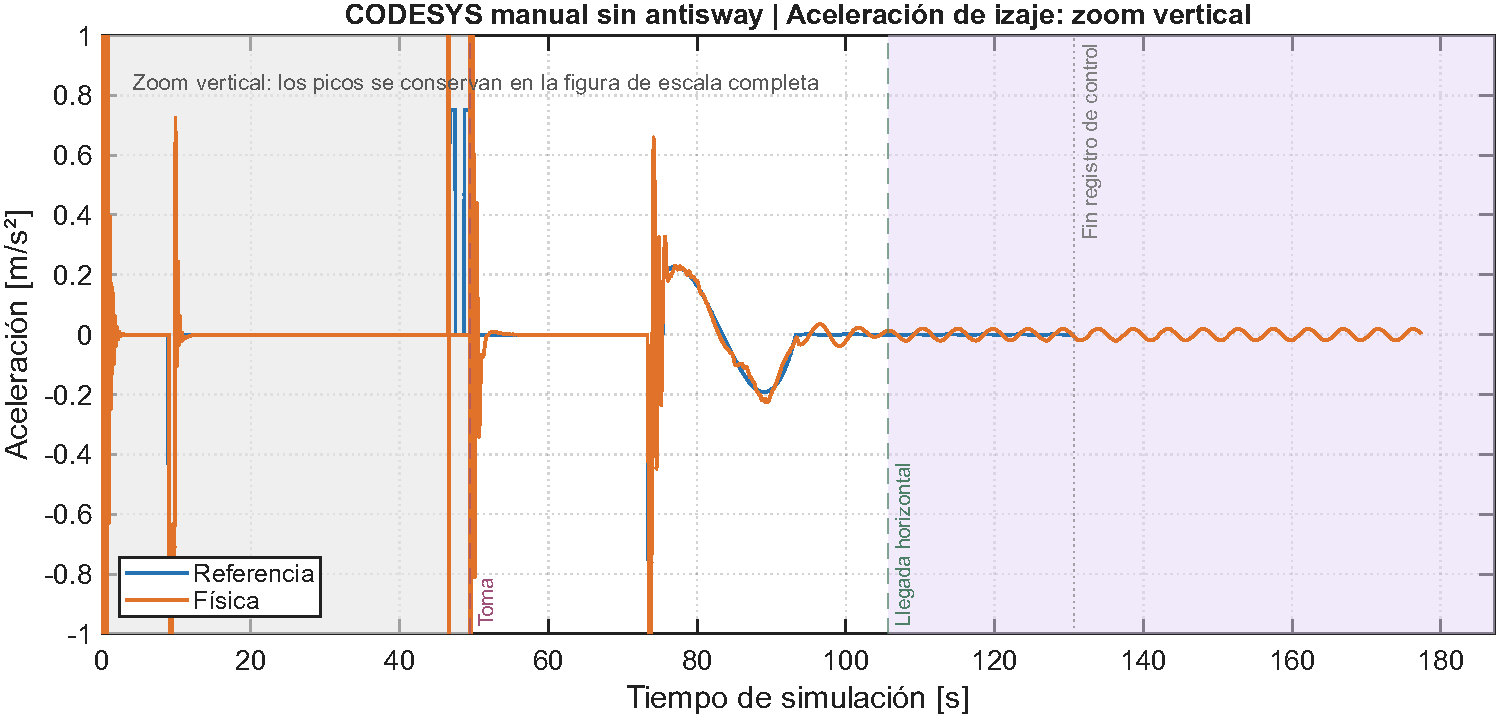
\includegraphics[width=0.98\textwidth]{graficas_individuales/manual_sin_ay_zoom.pdf}
\caption{CODESYS manual sin antisway: Aceleración de izaje con zoom vertical entre $-1$ y $+1~\mathrm{m/s^2}$ para observar su evolución temporal. Los picos que exceden este intervalo permanecen visibles en la figura de escala completa; no se filtraron las señales. Se respeta la cobertura parcial de las señales y no se extrapolan datos faltantes.}\label{fig:individual_manual_sin_ay_zoom}
\end{figure}

El balanceo residual observado es compatible con la espera de la compuerta de estabilidad. En el tramo físico disponible de $120$ a $177.305~\mathrm{s}$, el ángulo RMS fue $0.03169~\mathrm{rad}$ y el máximo absoluto $0.04521~\mathrm{rad}$; la velocidad angular RMS fue $0.02133~\mathrm{rad/s}$ y su máximo $0.03030~\mathrm{rad/s}$. Superar los umbrales angulares en parte de ese tramo no demuestra por sí solo una causa exclusiva del bloqueo. La contribución efectiva y la diferencia entre comando y referencia fueron exactamente cero en el registro nativo disponible hasta $130.72~\mathrm{s}$; no se extiende esa comprobación al tramo faltante.

\begin{figure}[!htbp]
\centering
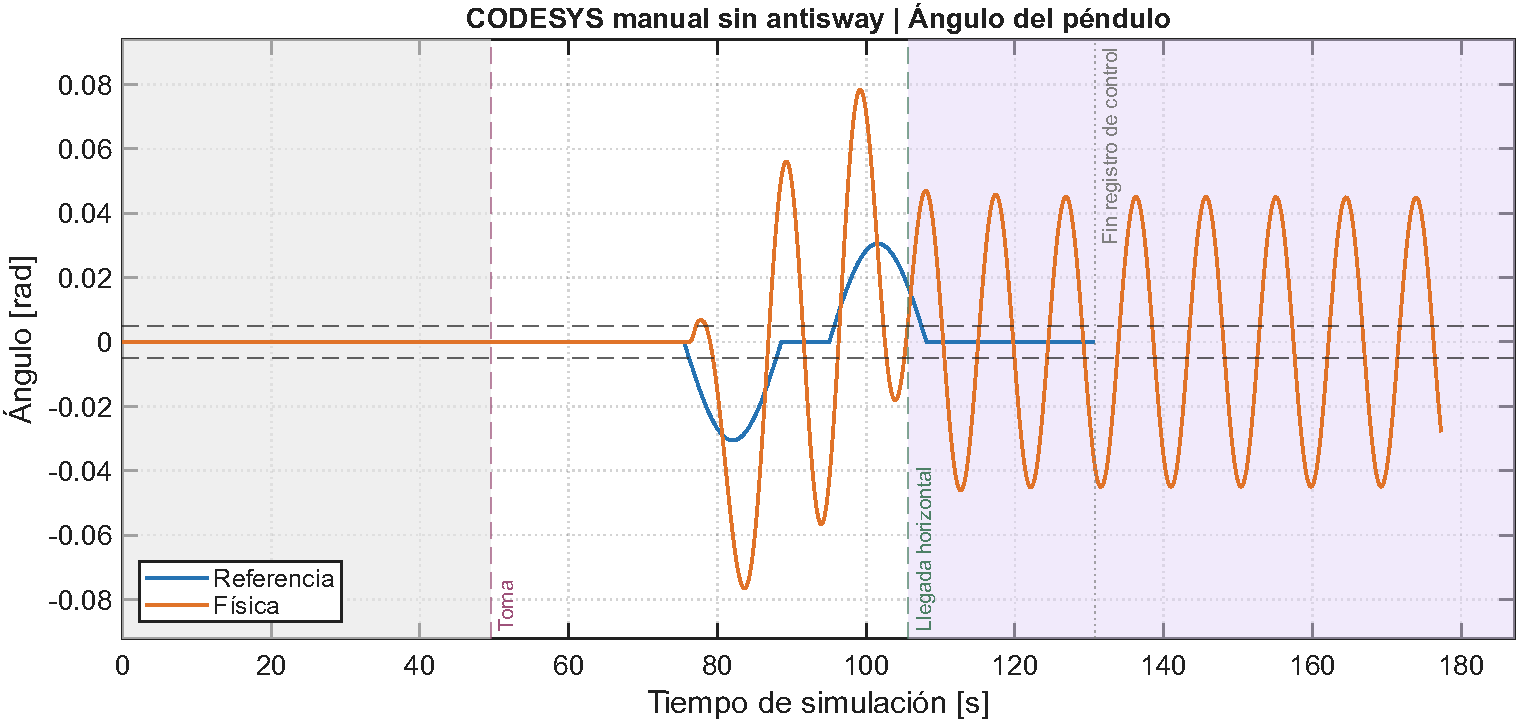
\includegraphics[width=0.98\textwidth]{graficas_individuales/manual_sin_theta.pdf}
\caption{CODESYS manual sin antisway: Ángulo físico y de referencia del péndulo. Las líneas horizontales señalan los umbrales angulares del descenso. Se respeta la cobertura parcial de las señales y no se extrapolan datos faltantes.}\label{fig:individual_manual_sin_theta}
\end{figure}

\begin{figure}[!htbp]
\centering
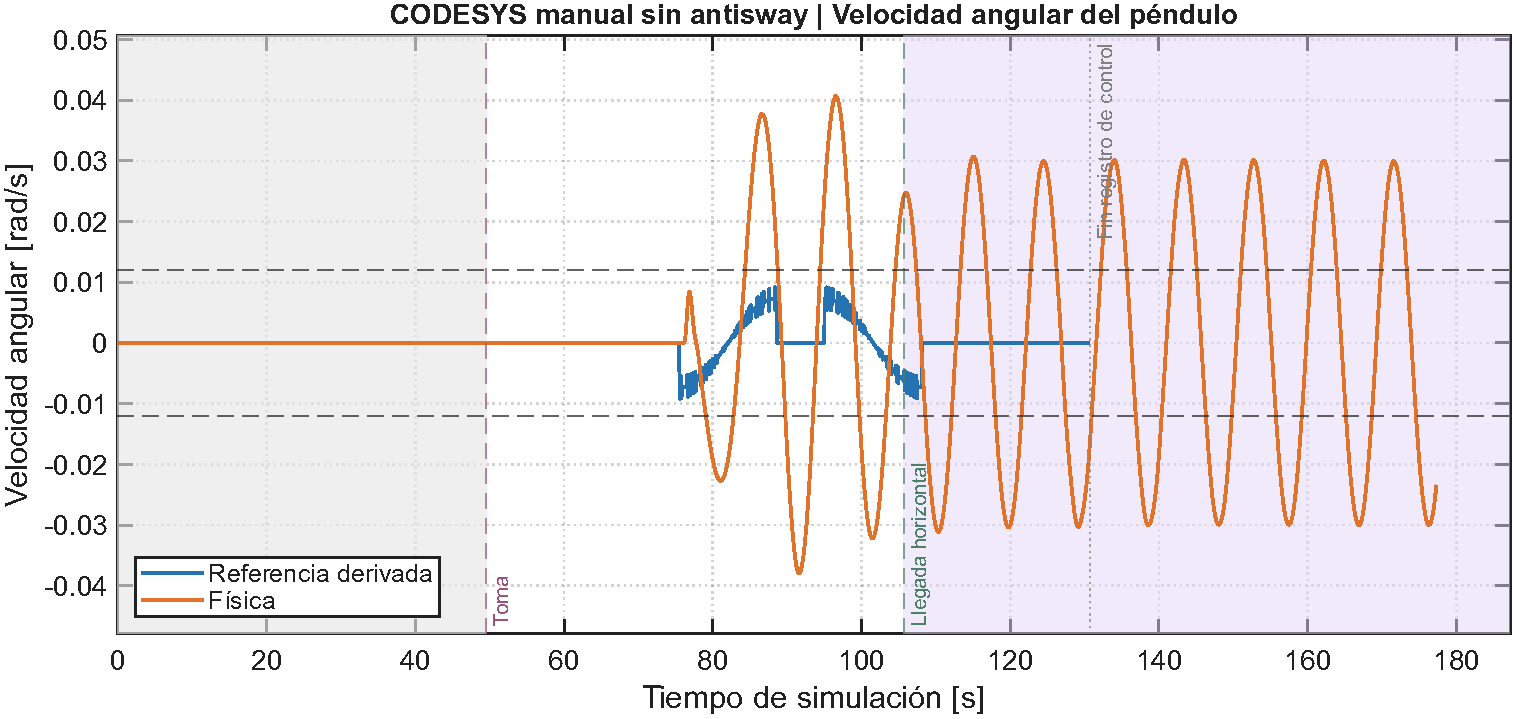
\includegraphics[width=0.98\textwidth]{graficas_individuales/manual_sin_omega.pdf}
\caption{CODESYS manual sin antisway: Velocidad angular física y referencia derivada numéricamente; se distinguen ambas fuentes. Las líneas horizontales indican los umbrales del descenso. Se respeta la cobertura parcial de las señales y no se extrapolan datos faltantes.}\label{fig:individual_manual_sin_omega}
\end{figure}

\begin{figure}[!htbp]
\centering
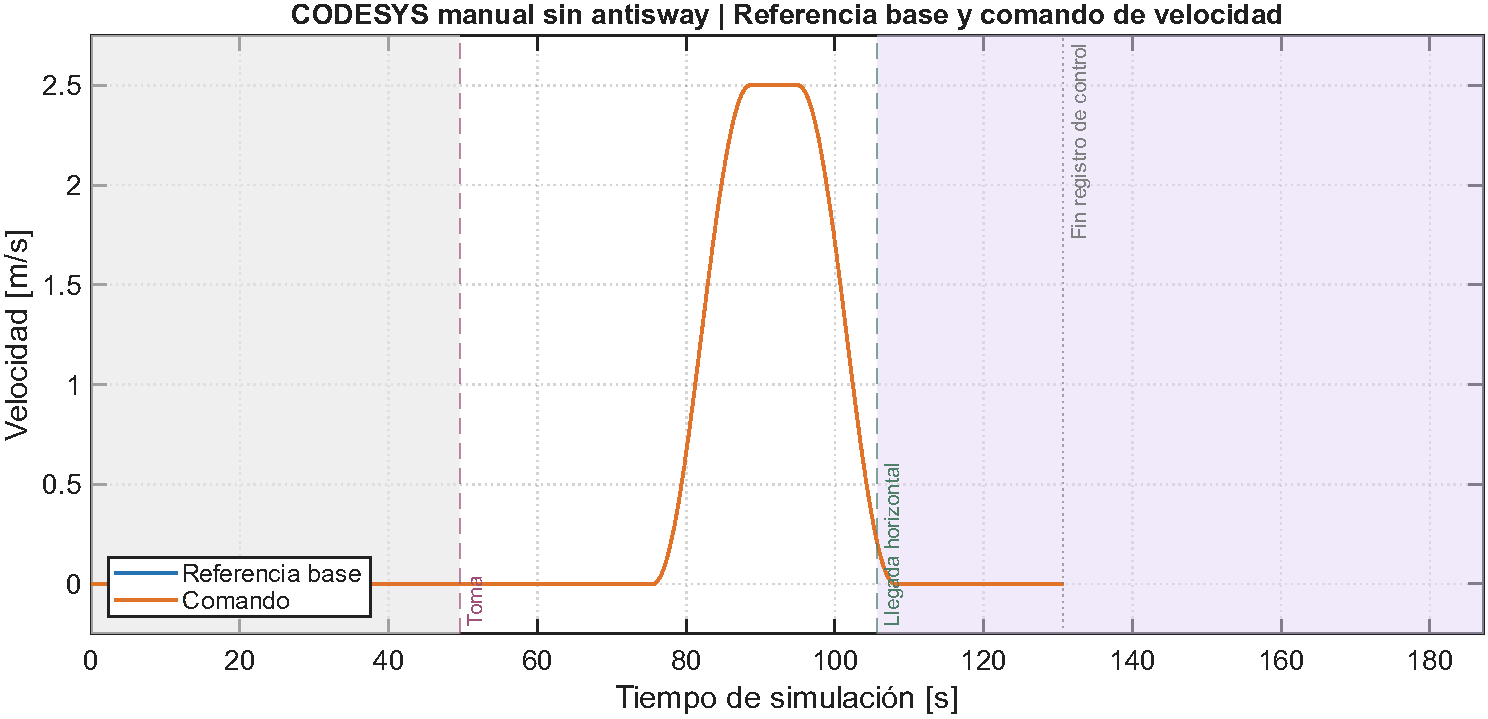
\includegraphics[width=0.98\textwidth]{graficas_individuales/manual_sin_vcmd.pdf}
\caption{CODESYS manual sin antisway: Referencia base y comando de velocidad; su diferencia corresponde a la contribución antisway efectiva en el sumador. Se respeta la cobertura parcial de las señales y no se extrapolan datos faltantes.}\label{fig:individual_manual_sin_vcmd}
\end{figure}

\begin{figure}[!htbp]
\centering
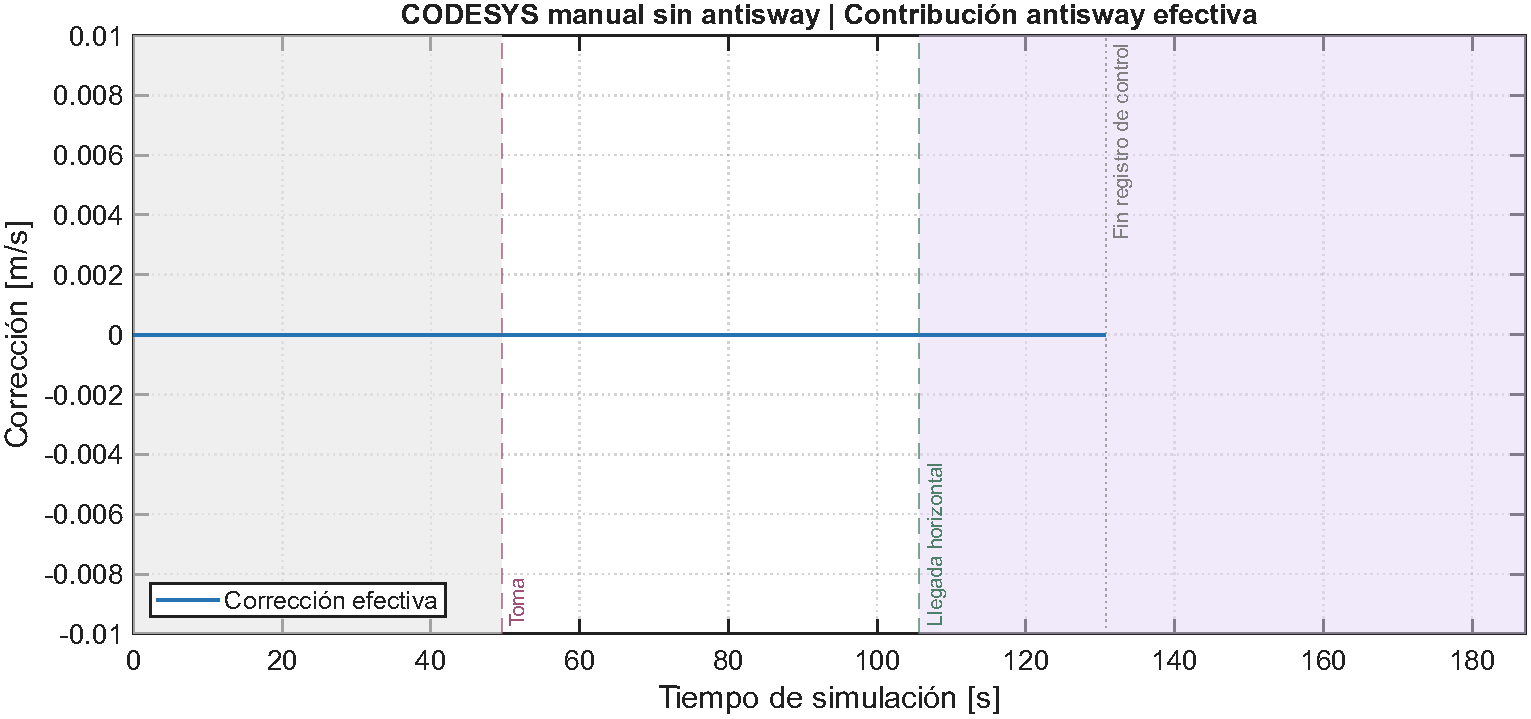
\includegraphics[width=0.98\textwidth]{graficas_individuales/manual_sin_sw.pdf}
\caption{CODESYS manual sin antisway: Contribución antisway efectivamente sumada al comando de velocidad. Se respeta la cobertura parcial de las señales y no se extrapolan datos faltantes.}\label{fig:individual_manual_sin_sw}
\end{figure}

Los torques diferencian la consigna del controlador y el torque físico de motor; su diferencia y los transitorios no se eliminan con filtrado posterior. Se muestra el arranque completo y una ampliación desde START para evitar que un pico inicial oculte el resto de la maniobra. La tensión permanece asociada a la carga suspendida en el tramo registrado. Los errores de posición se calculan sólo dentro de la cobertura común de referencia y señal física.

\begin{figure}[!htbp]
\centering
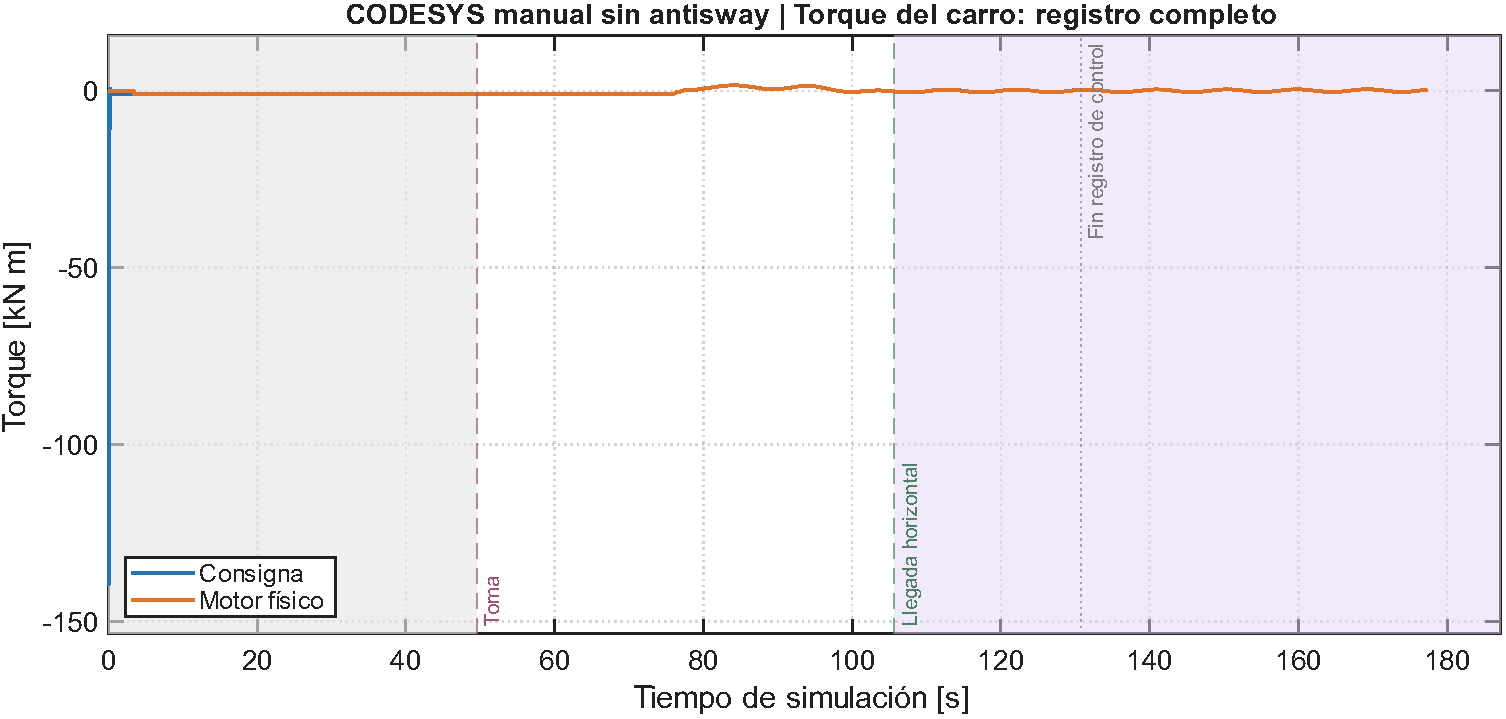
\includegraphics[width=0.98\textwidth]{graficas_individuales/manual_sin_tx.pdf}
\caption{CODESYS manual sin antisway: Consigna y torque físico del motor del carro en el intervalo representado, incluido el arranque.}\label{fig:individual_manual_sin_tx}
\end{figure}

\begin{figure}[!htbp]
\centering
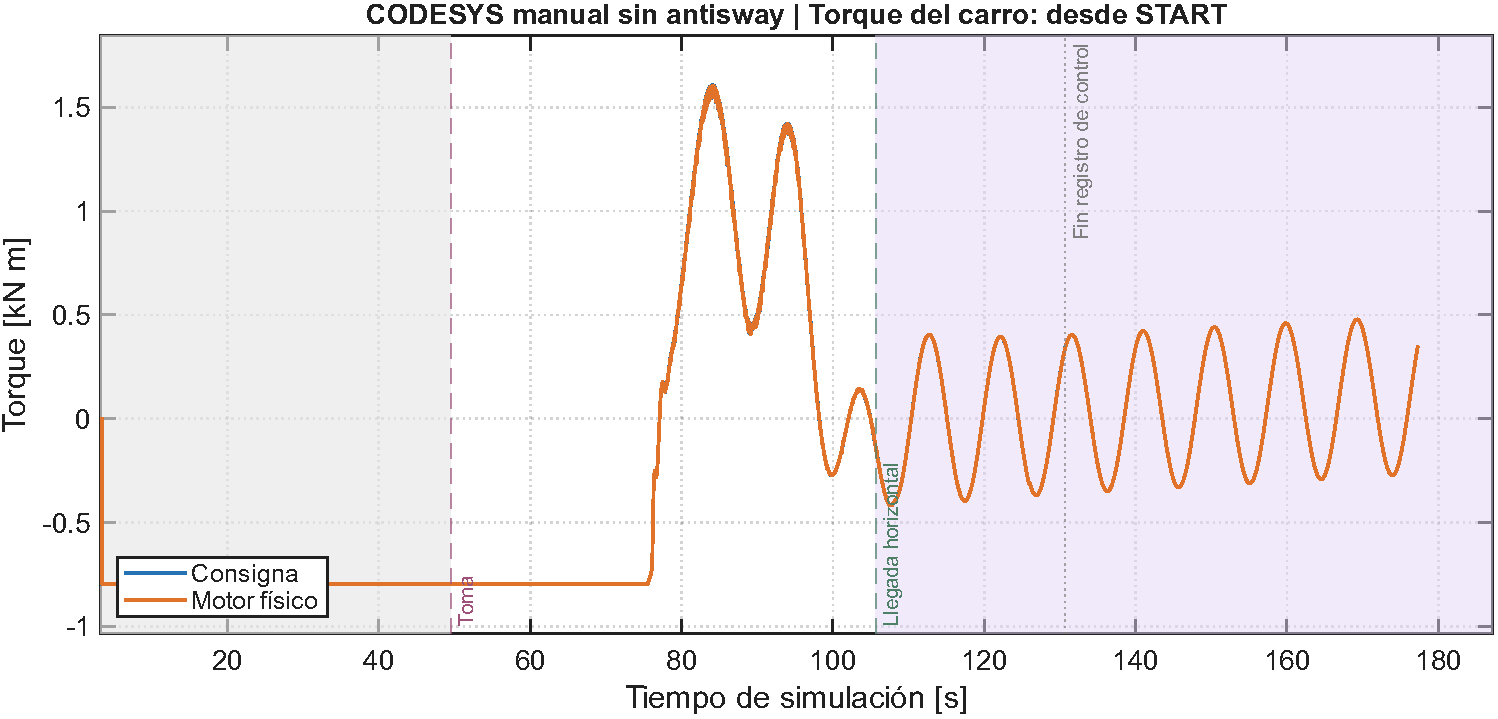
\includegraphics[width=0.98\textwidth]{graficas_individuales/manual_sin_tx_zoom.pdf}
\caption{CODESYS manual sin antisway: Consigna y torque físico del motor del carro desde START; la escala completa del arranque se conserva en una figura independiente.}\label{fig:individual_manual_sin_tx_zoom}
\end{figure}

\begin{figure}[!htbp]
\centering
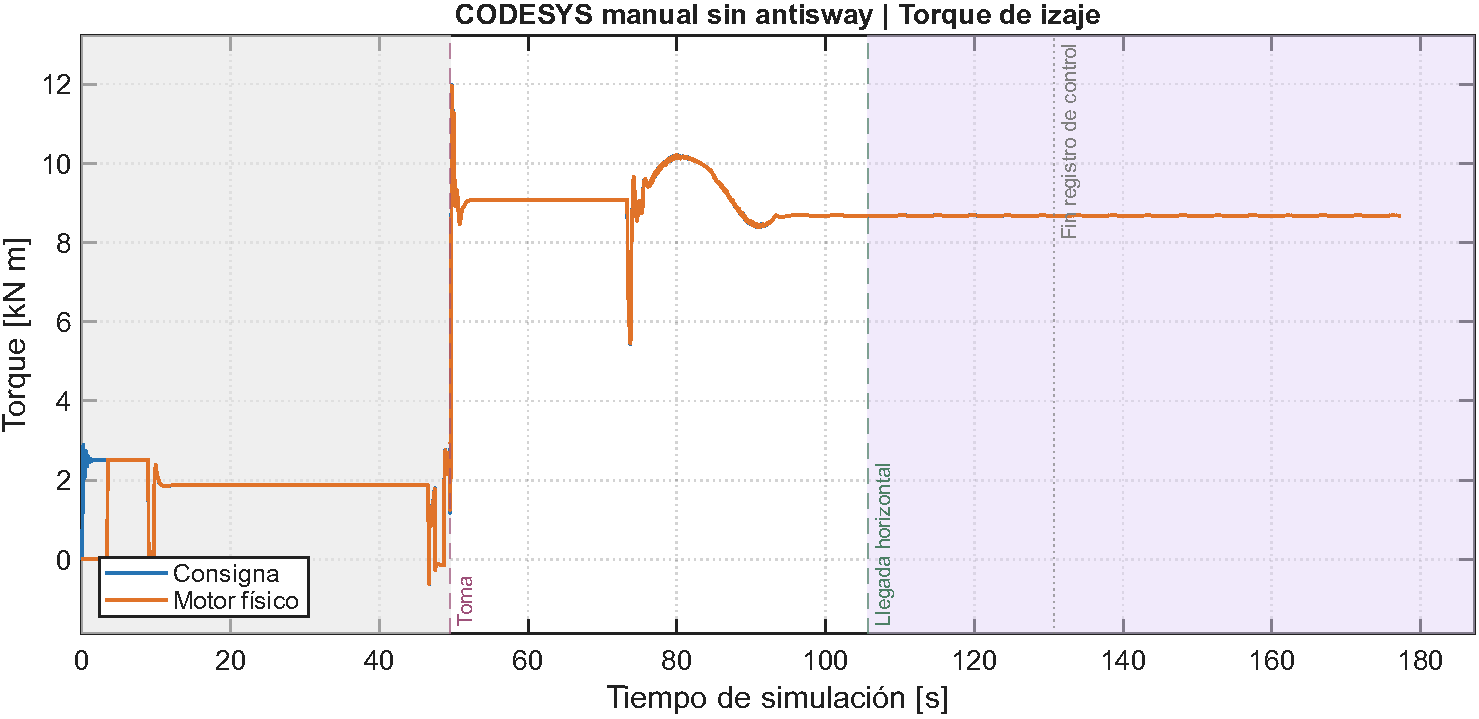
\includegraphics[width=0.98\textwidth]{graficas_individuales/manual_sin_ty.pdf}
\caption{CODESYS manual sin antisway: Consigna del controlador y torque físico del motor de izaje.}\label{fig:individual_manual_sin_ty}
\end{figure}

\begin{figure}[!htbp]
\centering
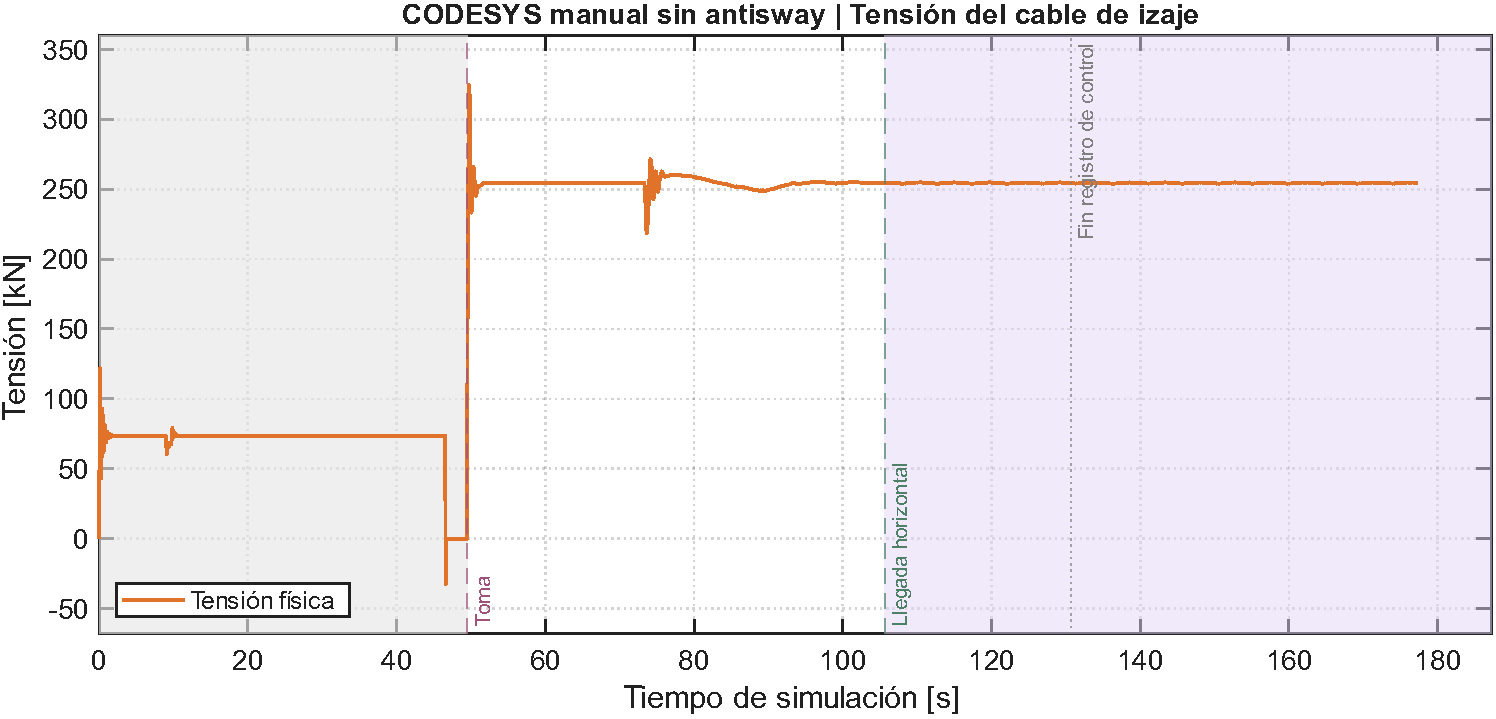
\includegraphics[width=0.98\textwidth]{graficas_individuales/manual_sin_tension.pdf}
\caption{CODESYS manual sin antisway: Tensión física del cable de izaje.}\label{fig:individual_manual_sin_tension}
\end{figure}

\begin{figure}[!htbp]
\centering
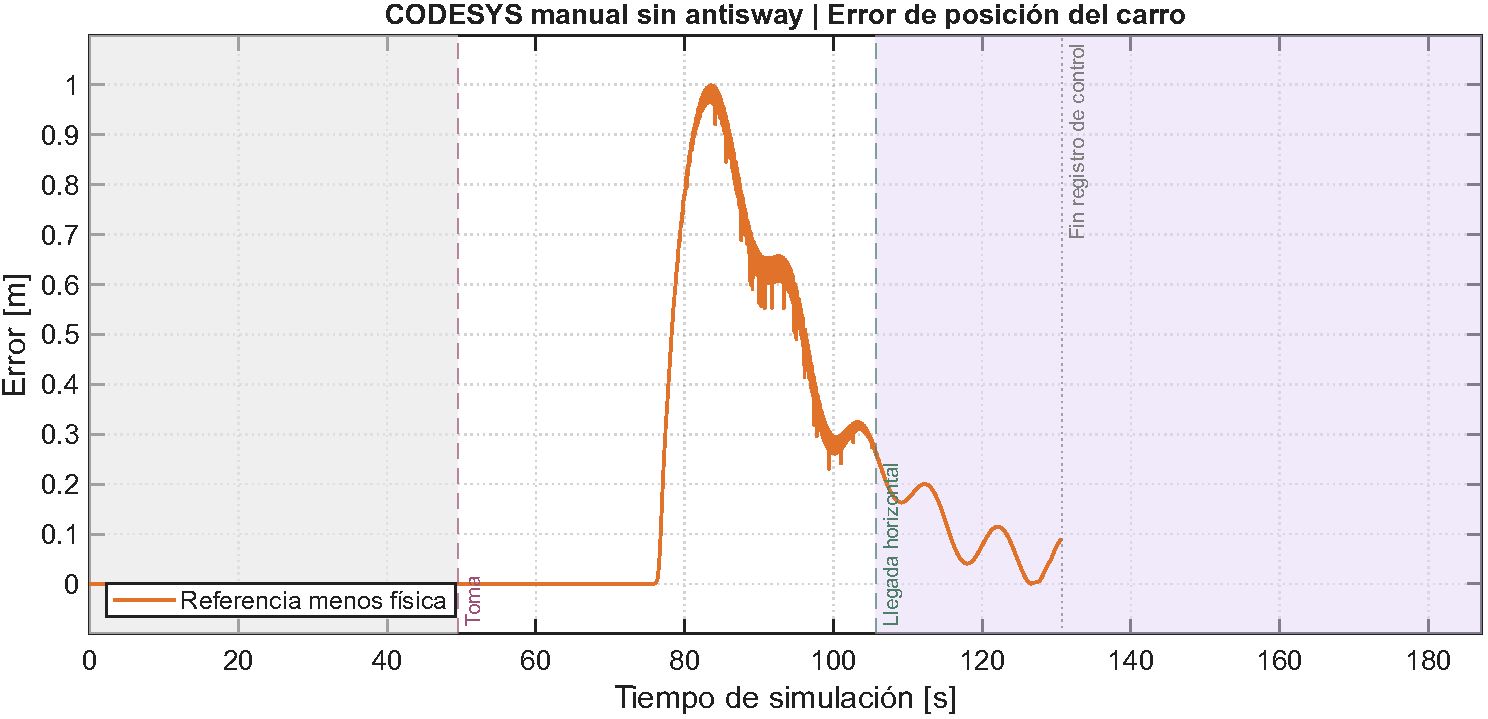
\includegraphics[width=0.98\textwidth]{graficas_individuales/manual_sin_ex.pdf}
\caption{CODESYS manual sin antisway: Error horizontal, calculado como referencia menos posición física. Se respeta la cobertura parcial de las señales y no se extrapolan datos faltantes.}\label{fig:individual_manual_sin_ex}
\end{figure}

\begin{figure}[!htbp]
\centering
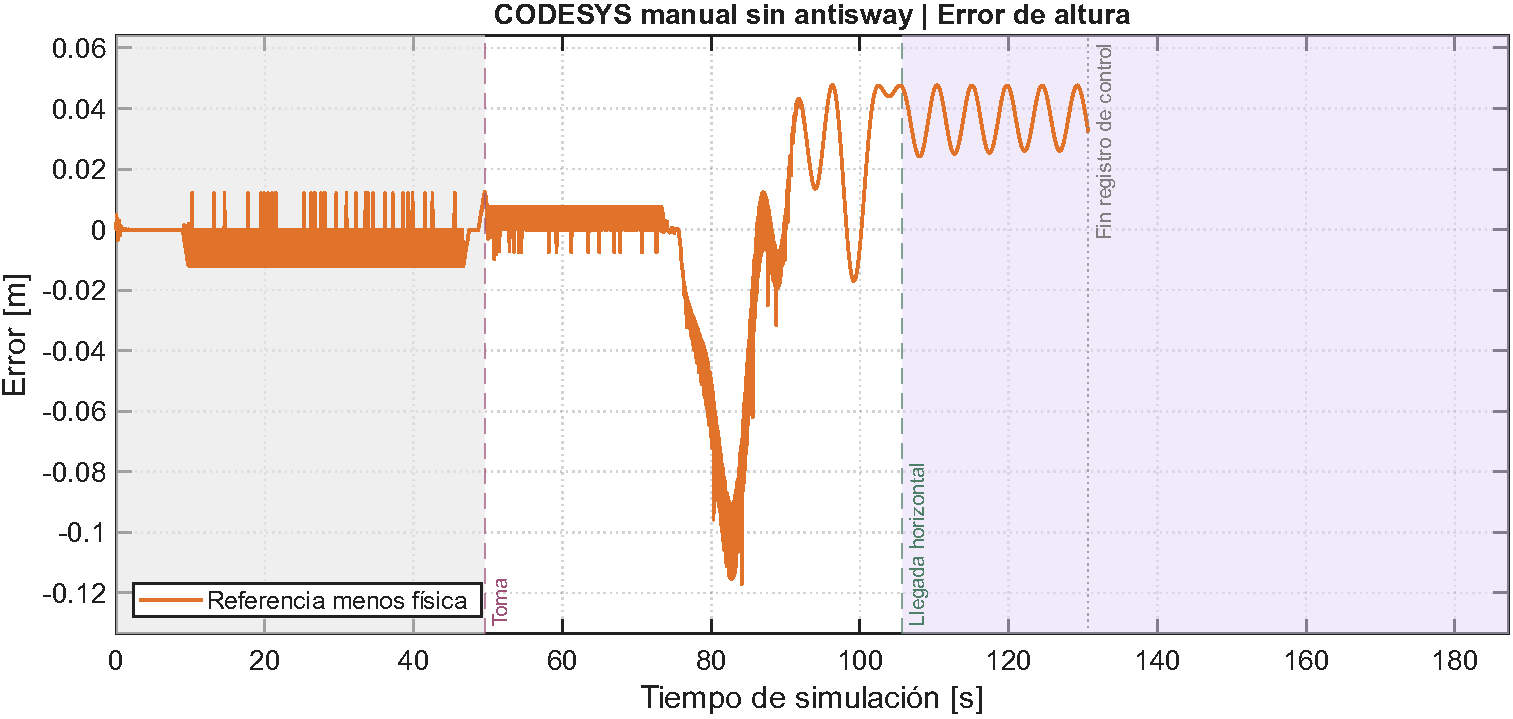
\includegraphics[width=0.98\textwidth]{graficas_individuales/manual_sin_ey.pdf}
\caption{CODESYS manual sin antisway: Error de altura, calculado como referencia menos altura física. Se respeta la cobertura parcial de las señales y no se extrapolan datos faltantes.}\label{fig:individual_manual_sin_ey}
\end{figure}

\begin{figure}[!htbp]
\centering
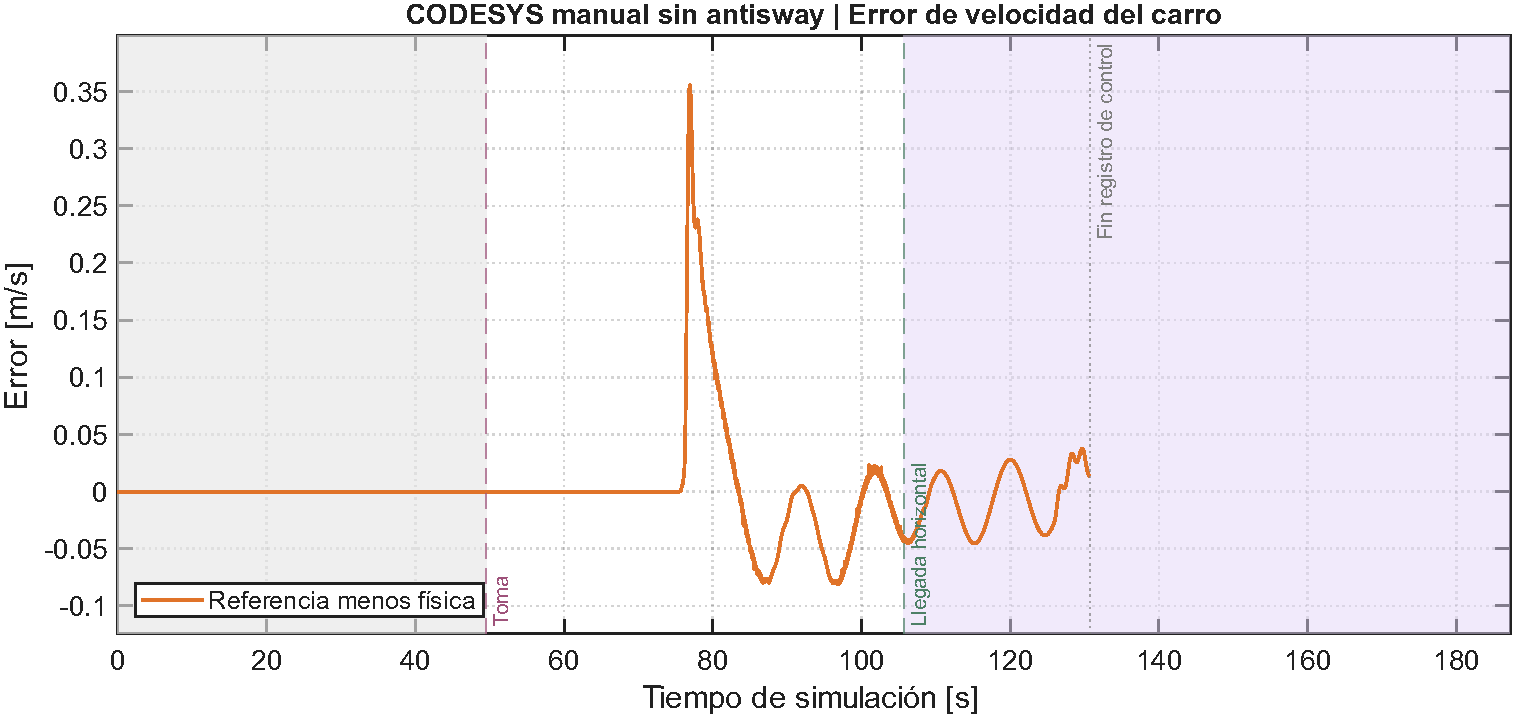
\includegraphics[width=0.98\textwidth]{graficas_individuales/manual_sin_evx.pdf}
\caption{CODESYS manual sin antisway: Error de velocidad del carro, calculado como referencia menos velocidad física. Se respeta la cobertura parcial de las señales y no se extrapolan datos faltantes.}\label{fig:individual_manual_sin_evx}
\end{figure}

\begin{figure}[!htbp]
\centering
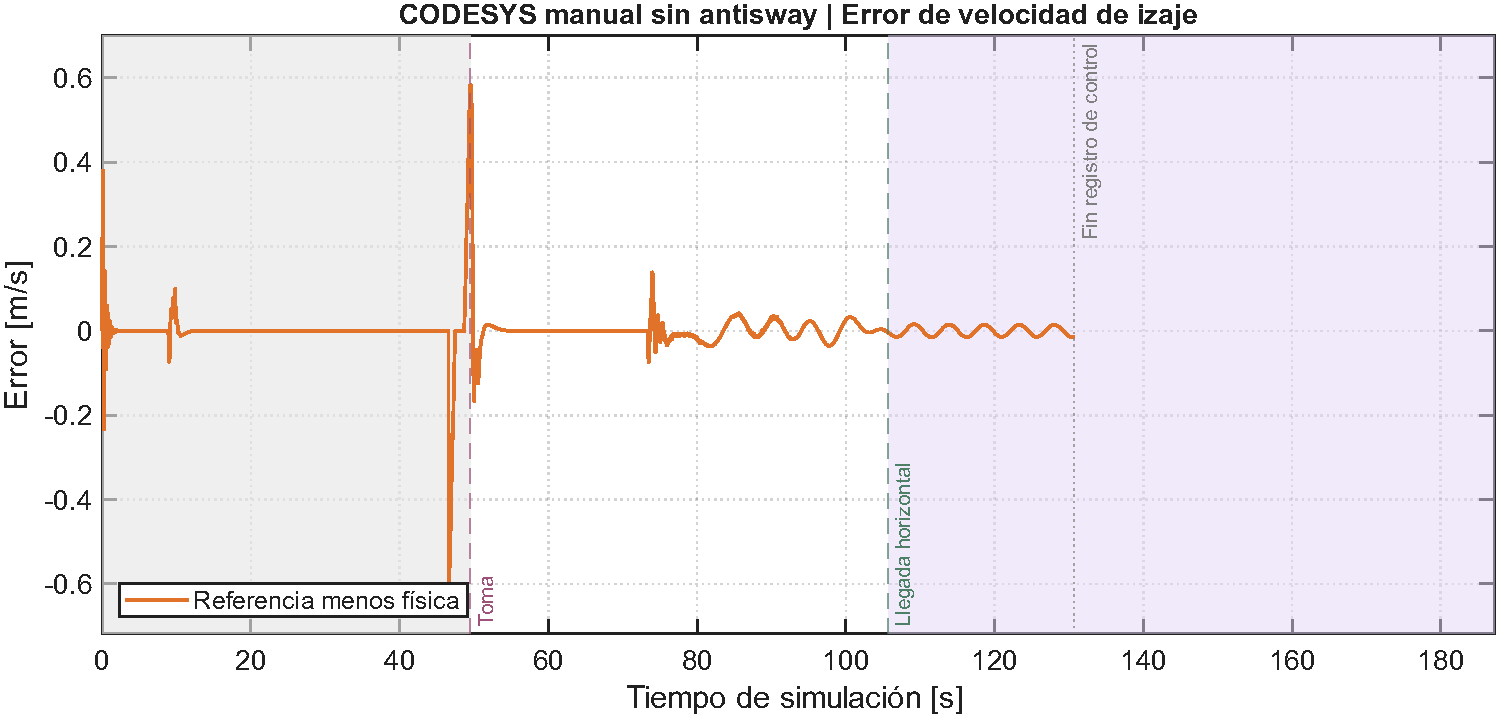
\includegraphics[width=0.98\textwidth]{graficas_individuales/manual_sin_evy.pdf}
\caption{CODESYS manual sin antisway: Error de velocidad de izaje, calculado como referencia menos velocidad física. Se respeta la cobertura parcial de las señales y no se extrapolan datos faltantes.}\label{fig:individual_manual_sin_evy}
\end{figure}

\begin{figure}[!htbp]
\centering
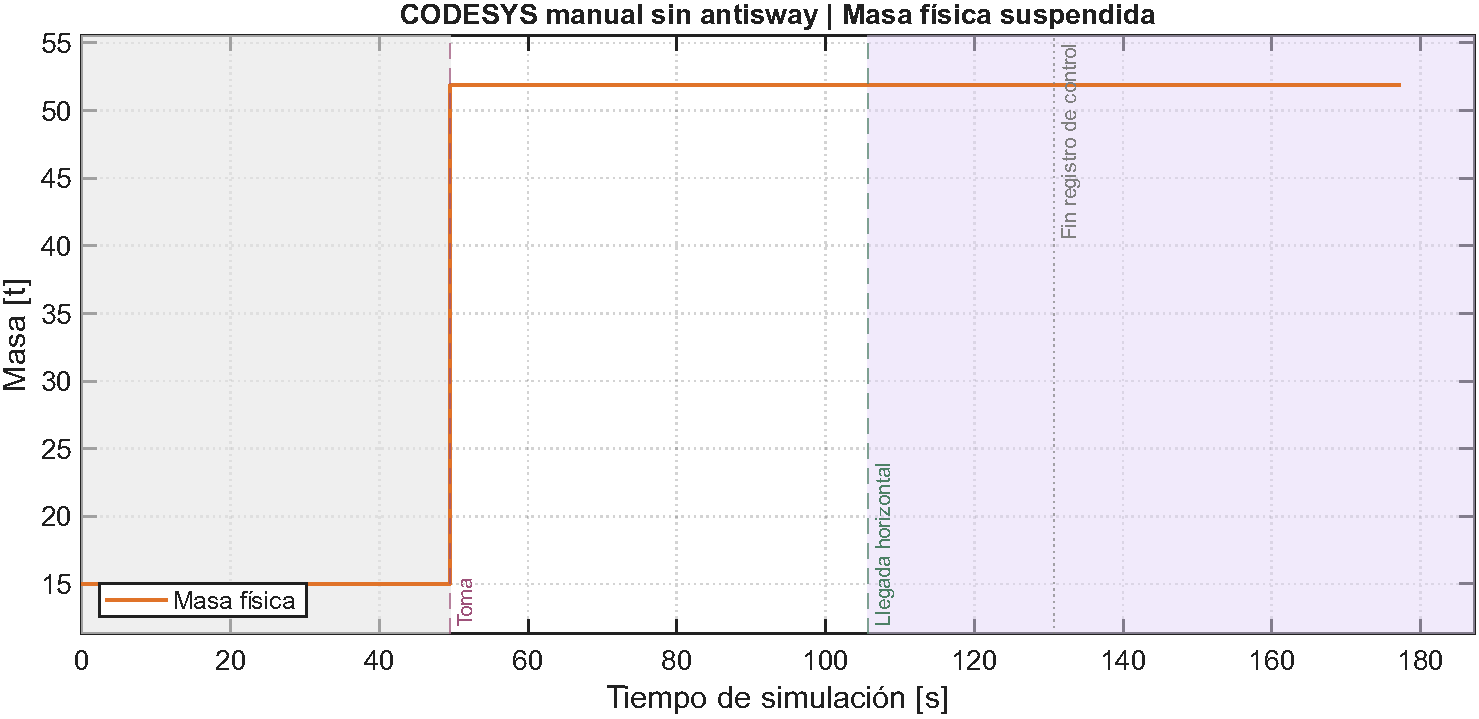
\includegraphics[width=0.98\textwidth]{graficas_individuales/manual_sin_masa.pdf}
\caption{CODESYS manual sin antisway: Masa física suspendida: 51,863 t representa conjunto cargado y 15 t corresponde al spreader vacío.}\label{fig:individual_manual_sin_masa}
\end{figure}

\begin{figure}[!htbp]
\centering
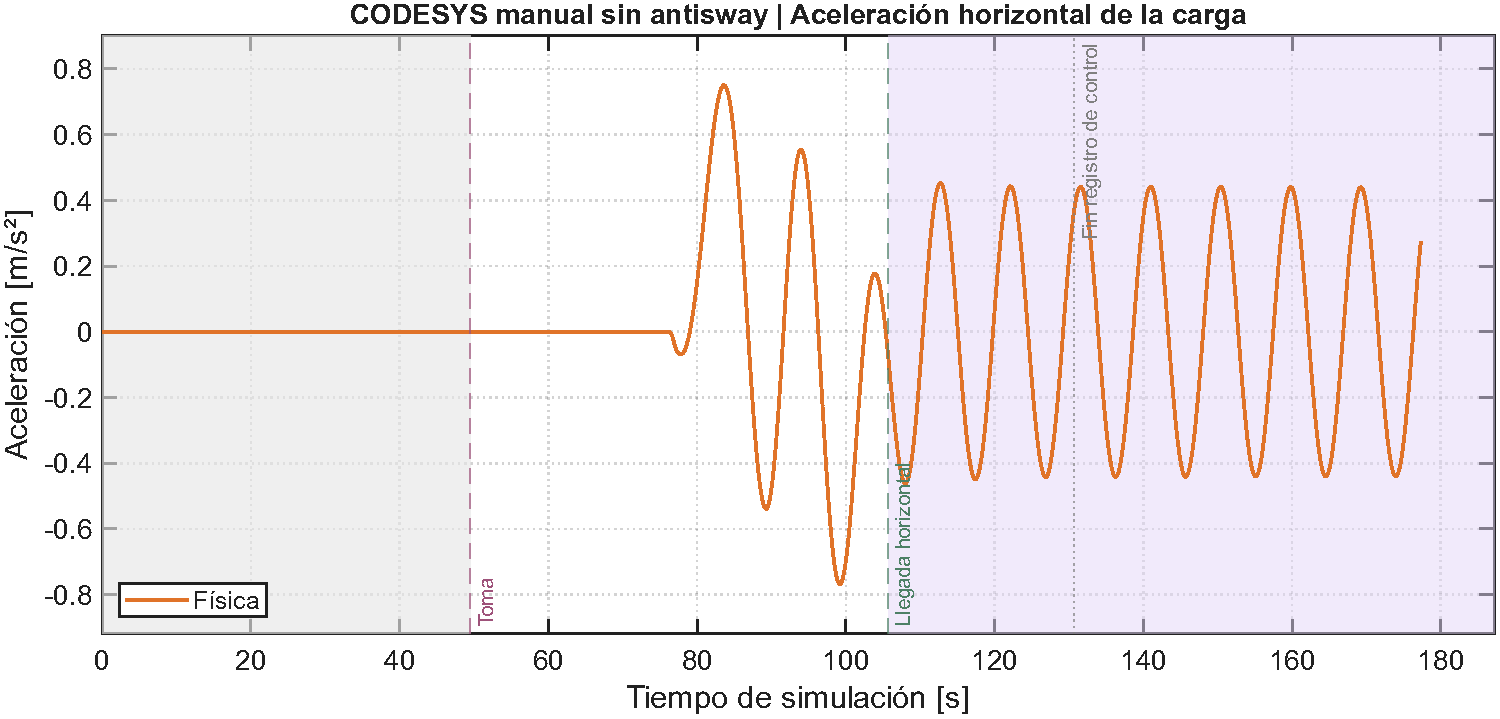
\includegraphics[width=0.98\textwidth]{graficas_individuales/manual_sin_ax_carga.pdf}
\caption{CODESYS manual sin antisway: Aceleración horizontal física de la carga; se conservan las oscilaciones registradas.}\label{fig:individual_manual_sin_ax_carga}
\end{figure}

\clearpage
\subsection{CODESYS manual con antisway: entrega física completada}
La secuencia inicial fue equivalente: START a $3.24~\mathrm{s}$, manual a $3.76~\mathrm{s}$, cierre solicitado a $46.64~\mathrm{s}$, masa cargada a $49.56~\mathrm{s}$ y despegue físico a $50.04~\mathrm{s}$. Automático se solicitó a $75.32~\mathrm{s}$ y fue observado por el operador a $75.44~\mathrm{s}$. La llegada horizontal ocurrió a $105.84~\mathrm{s}$; manual se solicitó a $133.24~\mathrm{s}$ y se observó a $133.32~\mathrm{s}$. El apoyo y apertura se solicitaron a $168.92~\mathrm{s}$, la entrega y STOP a $169.12~\mathrm{s}$, y la simulación terminó a $169.20~\mathrm{s}$.

Las posiciones y velocidades describen el cruce, el descenso automático habilitado y la aproximación manual final. Los picos de aceleración próximos al contacto pertenecen a la dinámica de apoyo y no se recortan. La corrección antisway modifica el comando respecto de la referencia base y reduce el balanceo hasta permitir el avance de la secuencia; su máximo nativo fue $0.46245~\mathrm{m/s}$. Esto no implica que todos los errores máximos de seguimiento sean menores.

\begin{figure}[!htbp]
\centering
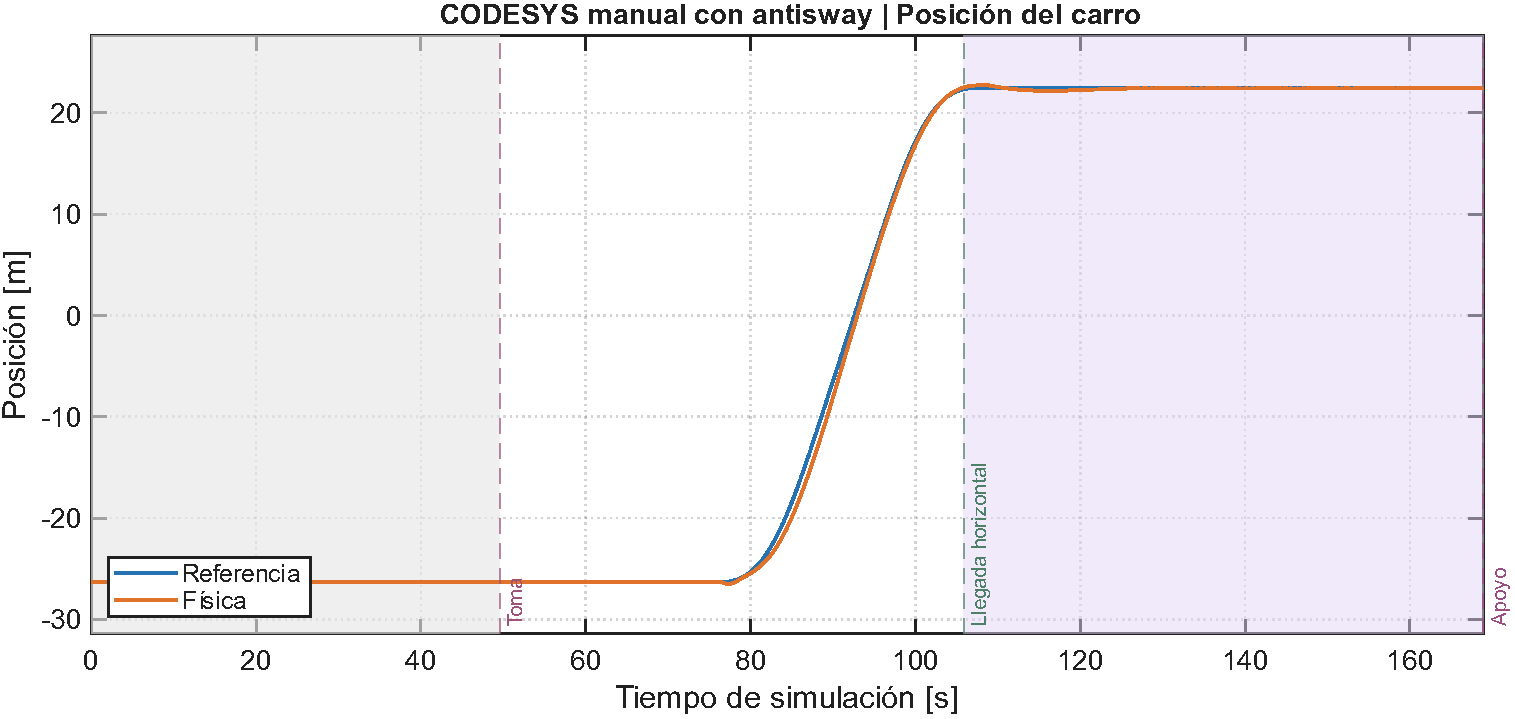
\includegraphics[width=0.98\textwidth]{graficas_individuales/manual_con_x.pdf}
\caption{CODESYS manual con antisway: Posición del carro: referencia y evolución física.}\label{fig:individual_manual_con_x}
\end{figure}

\begin{figure}[!htbp]
\centering
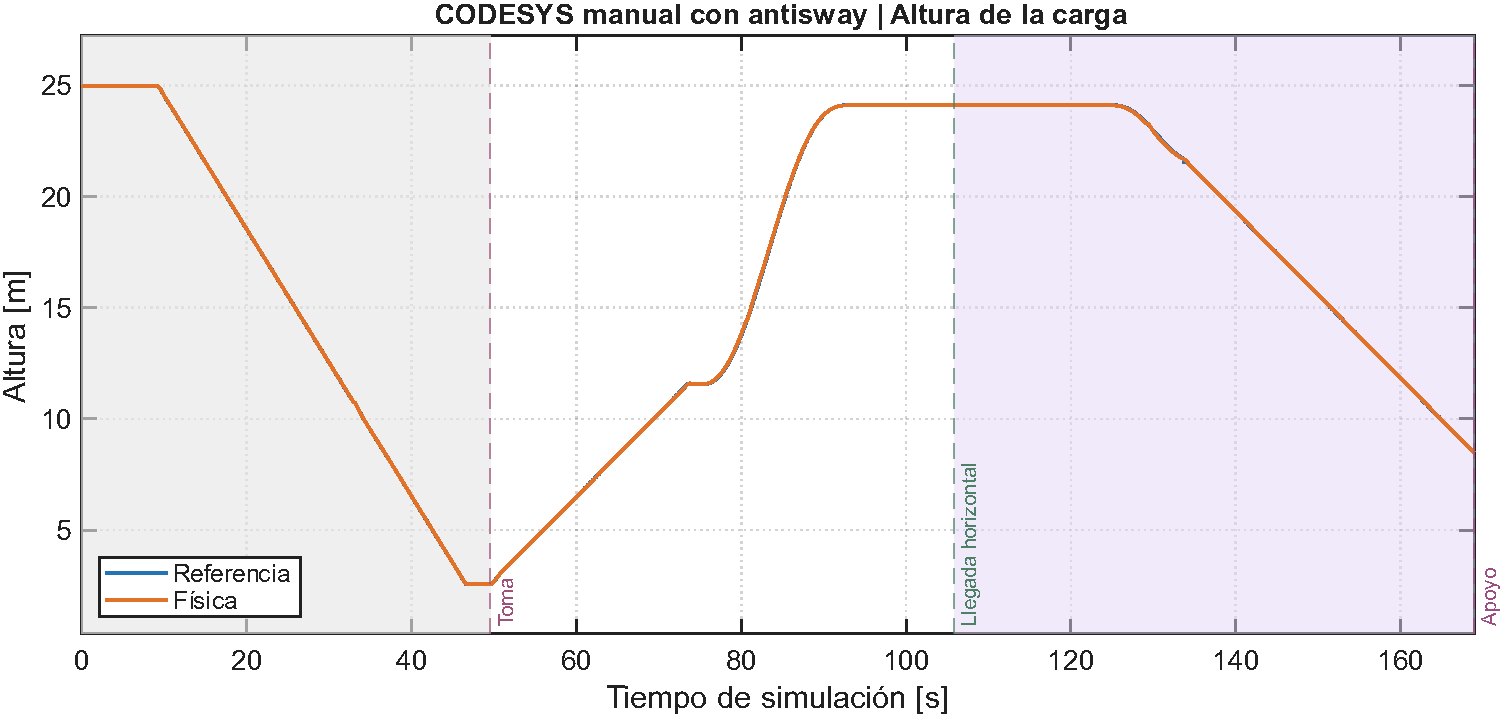
\includegraphics[width=0.98\textwidth]{graficas_individuales/manual_con_y.pdf}
\caption{CODESYS manual con antisway: Altura de la carga: referencia y evolución física.}\label{fig:individual_manual_con_y}
\end{figure}

\begin{figure}[!htbp]
\centering
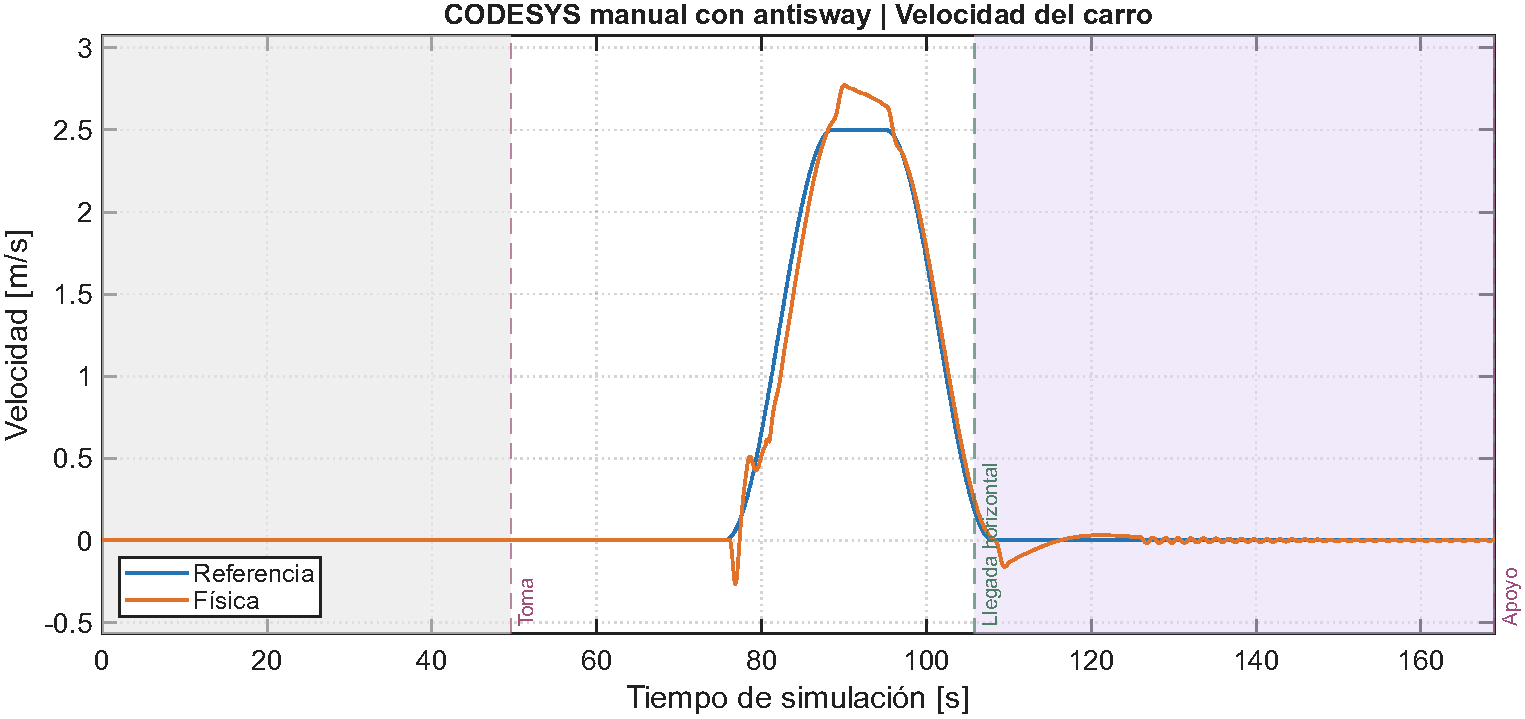
\includegraphics[width=0.98\textwidth]{graficas_individuales/manual_con_vx.pdf}
\caption{CODESYS manual con antisway: Velocidad del carro: referencia y señal física.}\label{fig:individual_manual_con_vx}
\end{figure}

\begin{figure}[!htbp]
\centering
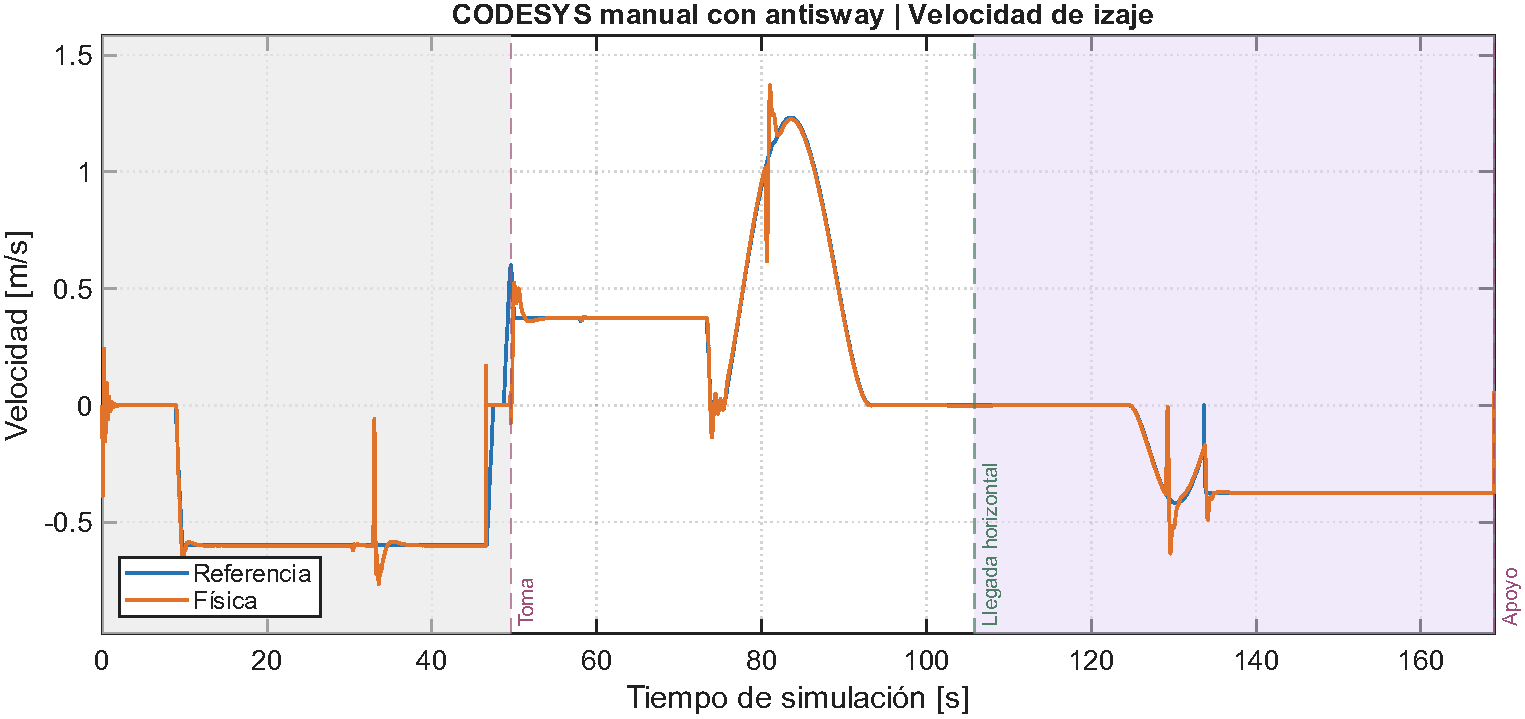
\includegraphics[width=0.98\textwidth]{graficas_individuales/manual_con_vy.pdf}
\caption{CODESYS manual con antisway: Velocidad de izaje: referencia y señal física.}\label{fig:individual_manual_con_vy}
\end{figure}

\begin{figure}[!htbp]
\centering
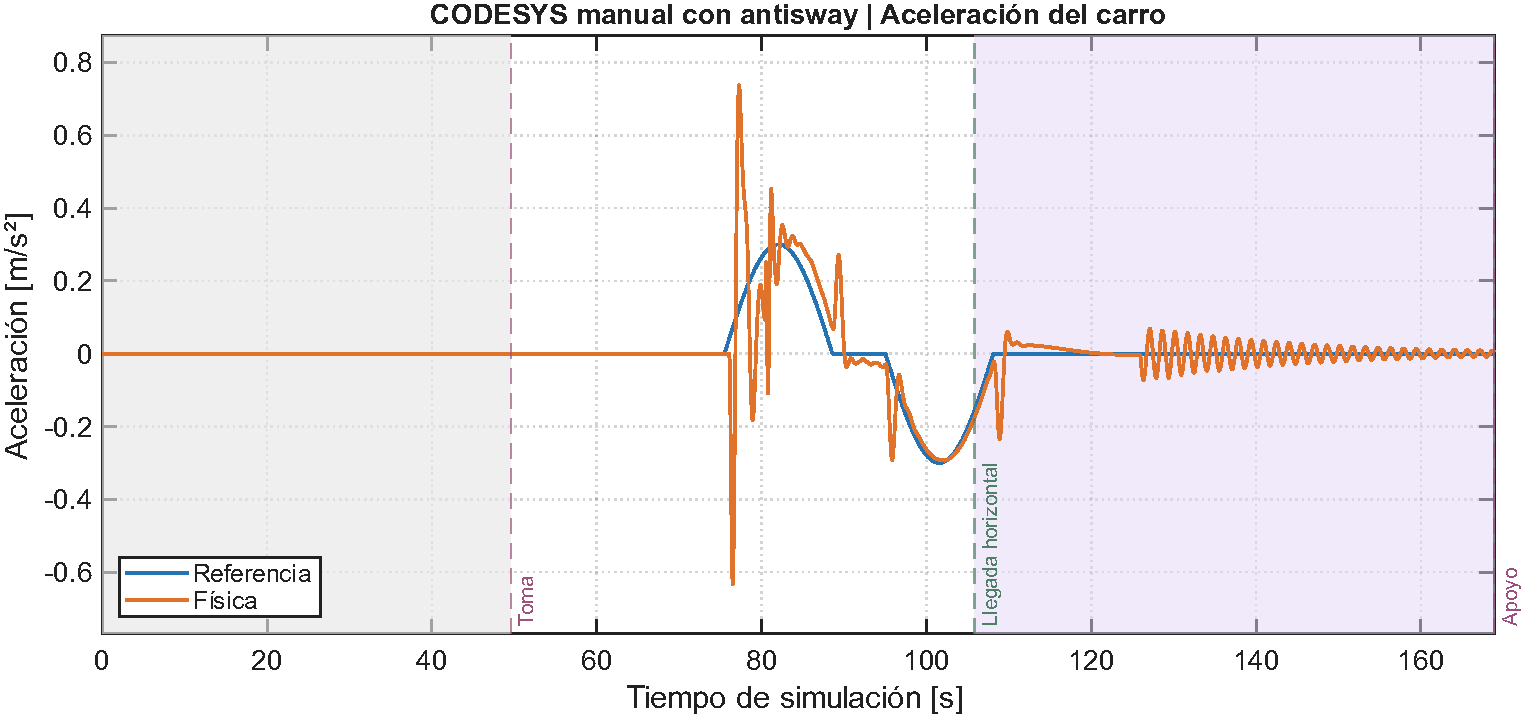
\includegraphics[width=0.98\textwidth]{graficas_individuales/manual_con_ax.pdf}
\caption{CODESYS manual con antisway: Aceleración del carro: referencia y señal física.}\label{fig:individual_manual_con_ax}
\end{figure}

\begin{figure}[!htbp]
\centering
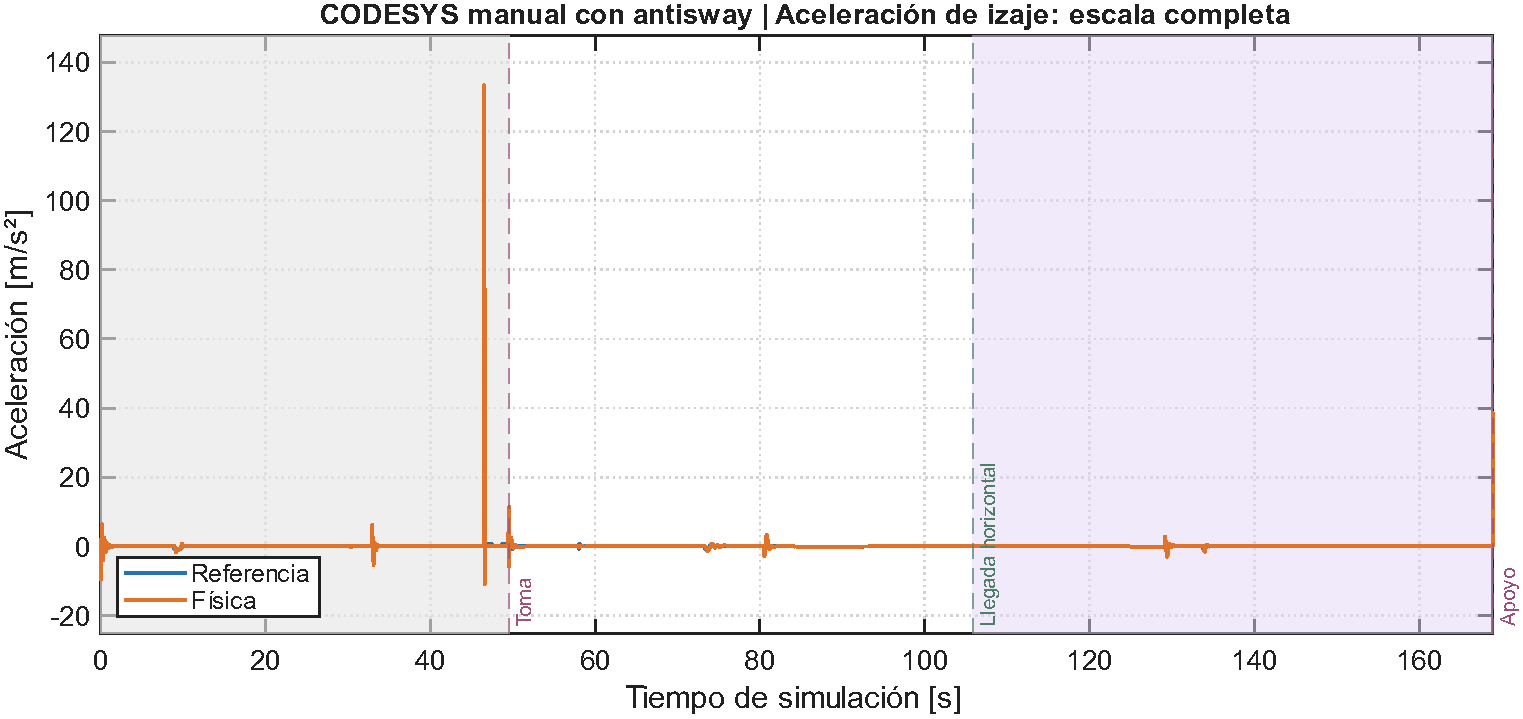
\includegraphics[width=0.98\textwidth]{graficas_individuales/manual_con_ay.pdf}
\caption{CODESYS manual con antisway: Aceleración de izaje en escala completa; se conservan los picos de contacto y arranque.}\label{fig:individual_manual_con_ay}
\end{figure}

\begin{figure}[!htbp]
\centering
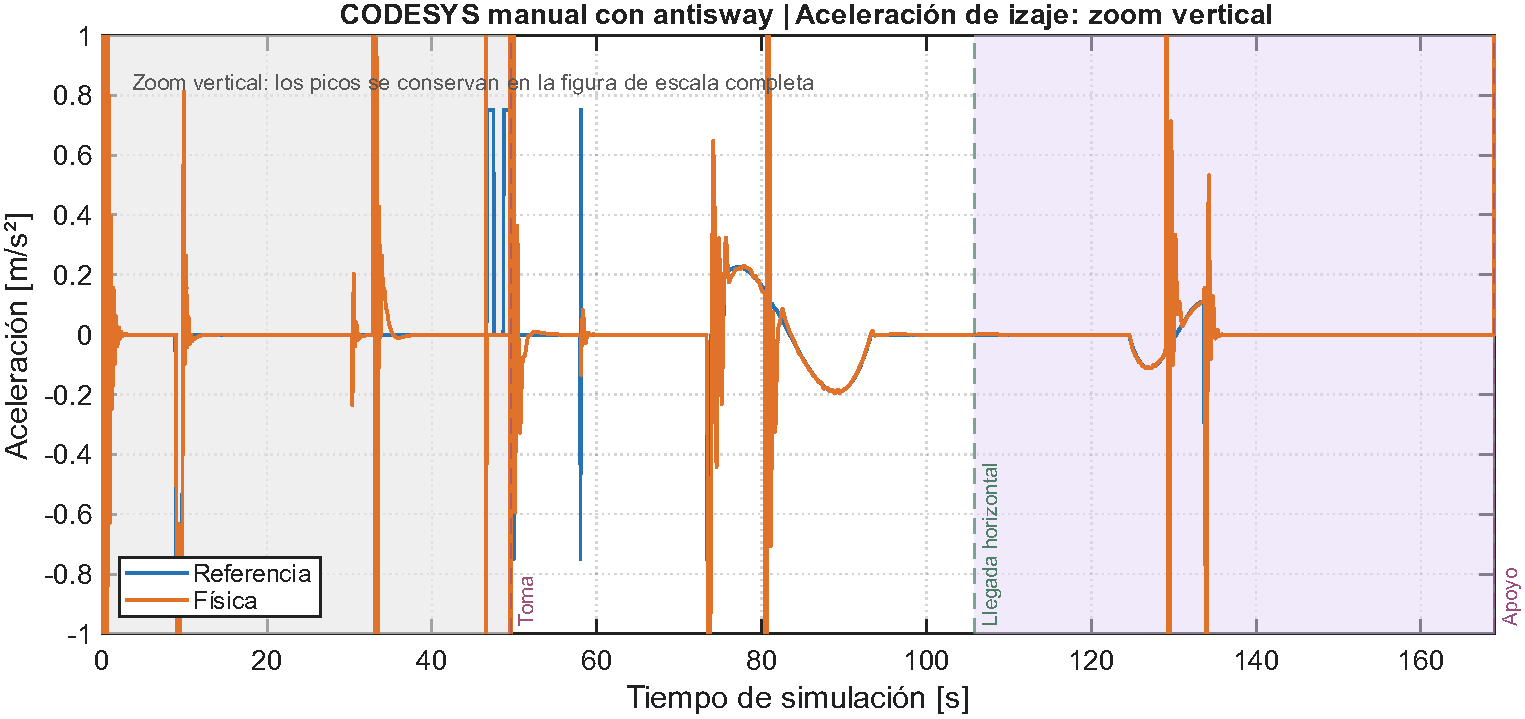
\includegraphics[width=0.98\textwidth]{graficas_individuales/manual_con_ay_zoom.pdf}
\caption{CODESYS manual con antisway: Aceleración de izaje con zoom vertical entre $-1$ y $+1~\mathrm{m/s^2}$ para observar su evolución temporal. Los picos que exceden este intervalo permanecen visibles en la figura de escala completa; no se filtraron las señales.}\label{fig:individual_manual_con_ay_zoom}
\end{figure}

\begin{figure}[!htbp]
\centering
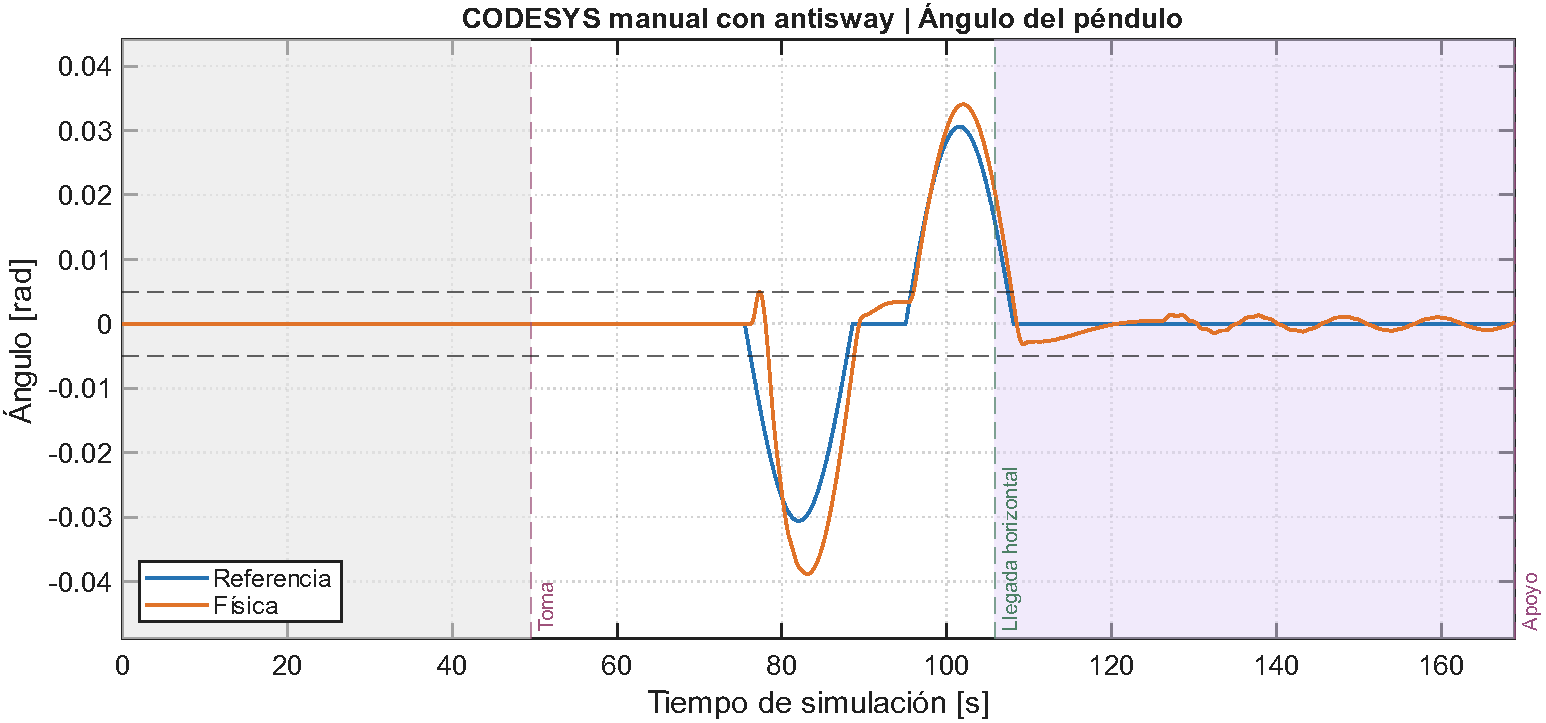
\includegraphics[width=0.98\textwidth]{graficas_individuales/manual_con_theta.pdf}
\caption{CODESYS manual con antisway: Ángulo físico y de referencia del péndulo. Las líneas horizontales señalan los umbrales angulares del descenso.}\label{fig:individual_manual_con_theta}
\end{figure}

\begin{figure}[!htbp]
\centering
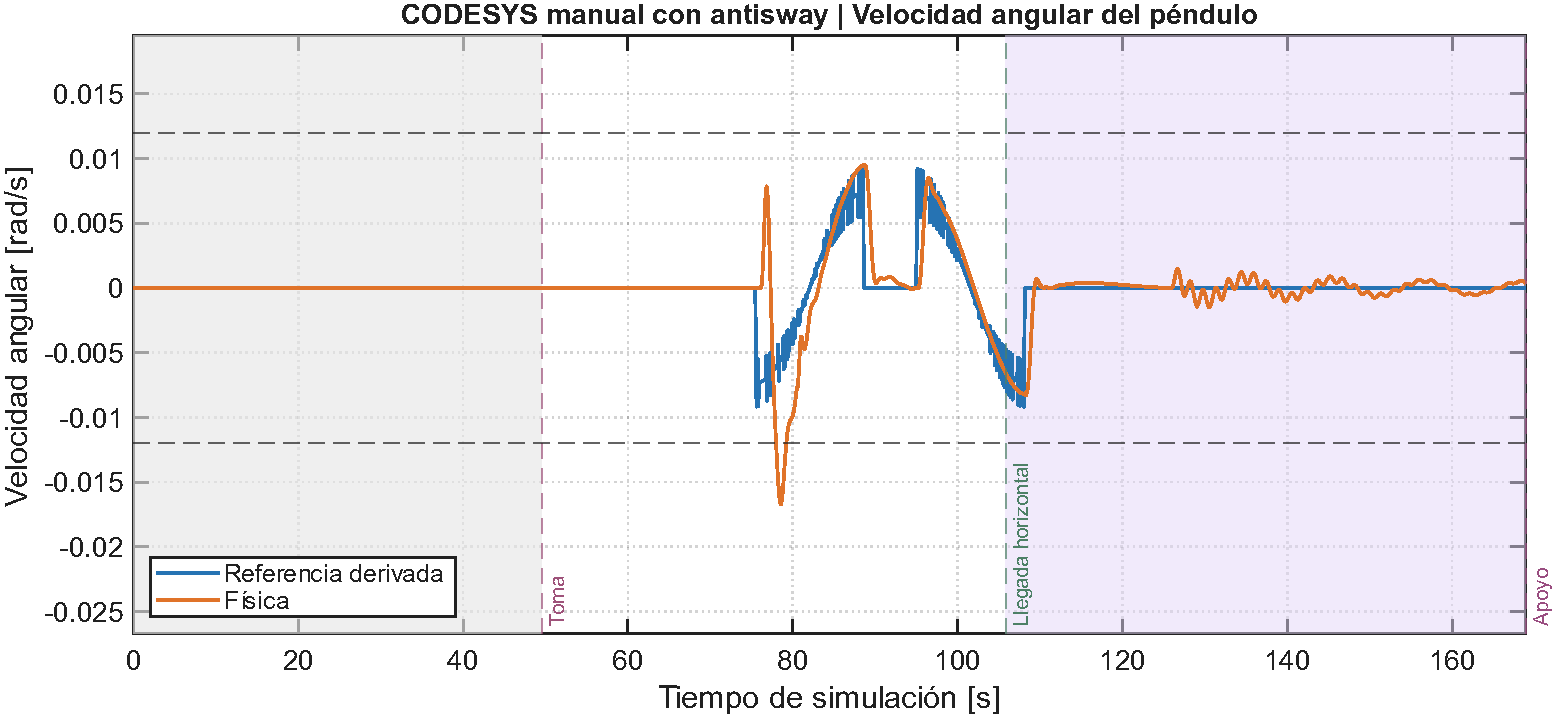
\includegraphics[width=0.98\textwidth]{graficas_individuales/manual_con_omega.pdf}
\caption{CODESYS manual con antisway: Velocidad angular física y referencia derivada numéricamente; se distinguen ambas fuentes. Las líneas horizontales indican los umbrales del descenso.}\label{fig:individual_manual_con_omega}
\end{figure}

\begin{figure}[!htbp]
\centering
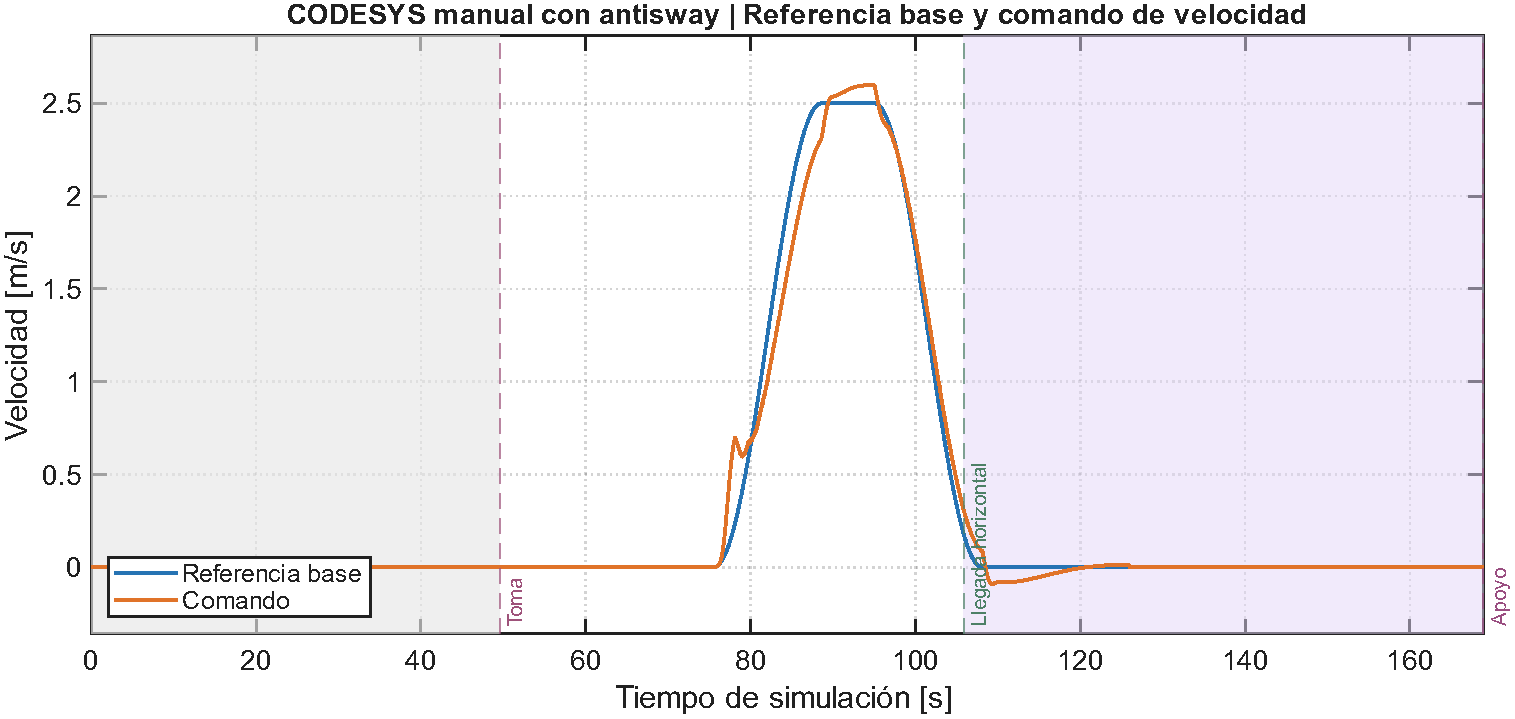
\includegraphics[width=0.98\textwidth]{graficas_individuales/manual_con_vcmd.pdf}
\caption{CODESYS manual con antisway: Referencia base y comando de velocidad; su diferencia corresponde a la contribución antisway efectiva en el sumador.}\label{fig:individual_manual_con_vcmd}
\end{figure}

\begin{figure}[!htbp]
\centering
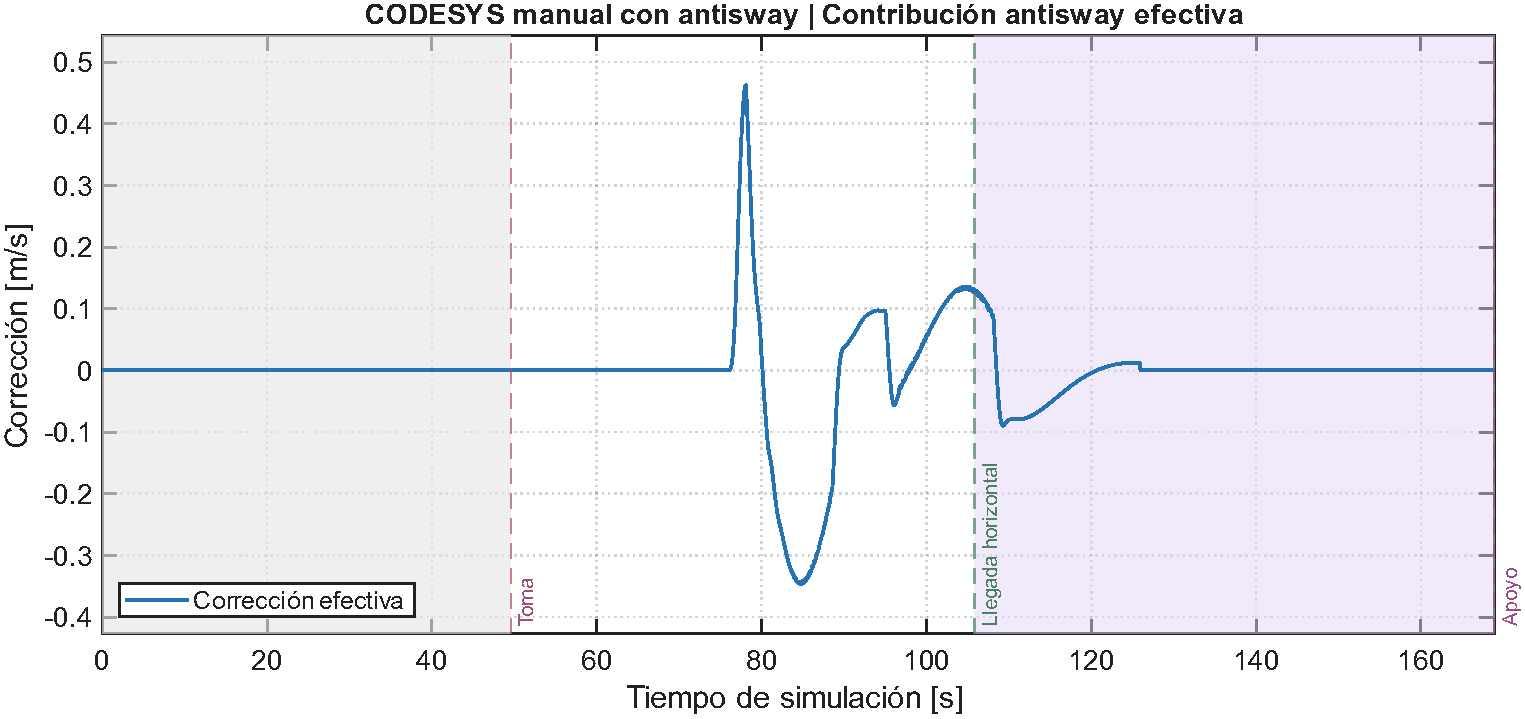
\includegraphics[width=0.98\textwidth]{graficas_individuales/manual_con_sw.pdf}
\caption{CODESYS manual con antisway: Contribución antisway efectivamente sumada al comando de velocidad.}\label{fig:individual_manual_con_sw}
\end{figure}

La masa física pasa del conjunto cargado al spreader vacío: $15\,000~\mathrm{kg}$ al final. El origen disminuye $2.59~\mathrm{m}$ y el destino aumenta $2.59~\mathrm{m}$. La posición final del carro fue $22.41138~\mathrm{m}$ y la altura $8.50636~\mathrm{m}$; el error horizontal al centro fue $0.04862~\mathrm{m}$. Estos datos confirman entrega física, además de la apertura de twistlocks. Los torques y la tensión muestran la respuesta al movimiento y al apoyo; la caída de masa distingue esta corrida de una llegada sin descarga. El registro físico y de control cubre la parada.

\begin{figure}[!htbp]
\centering
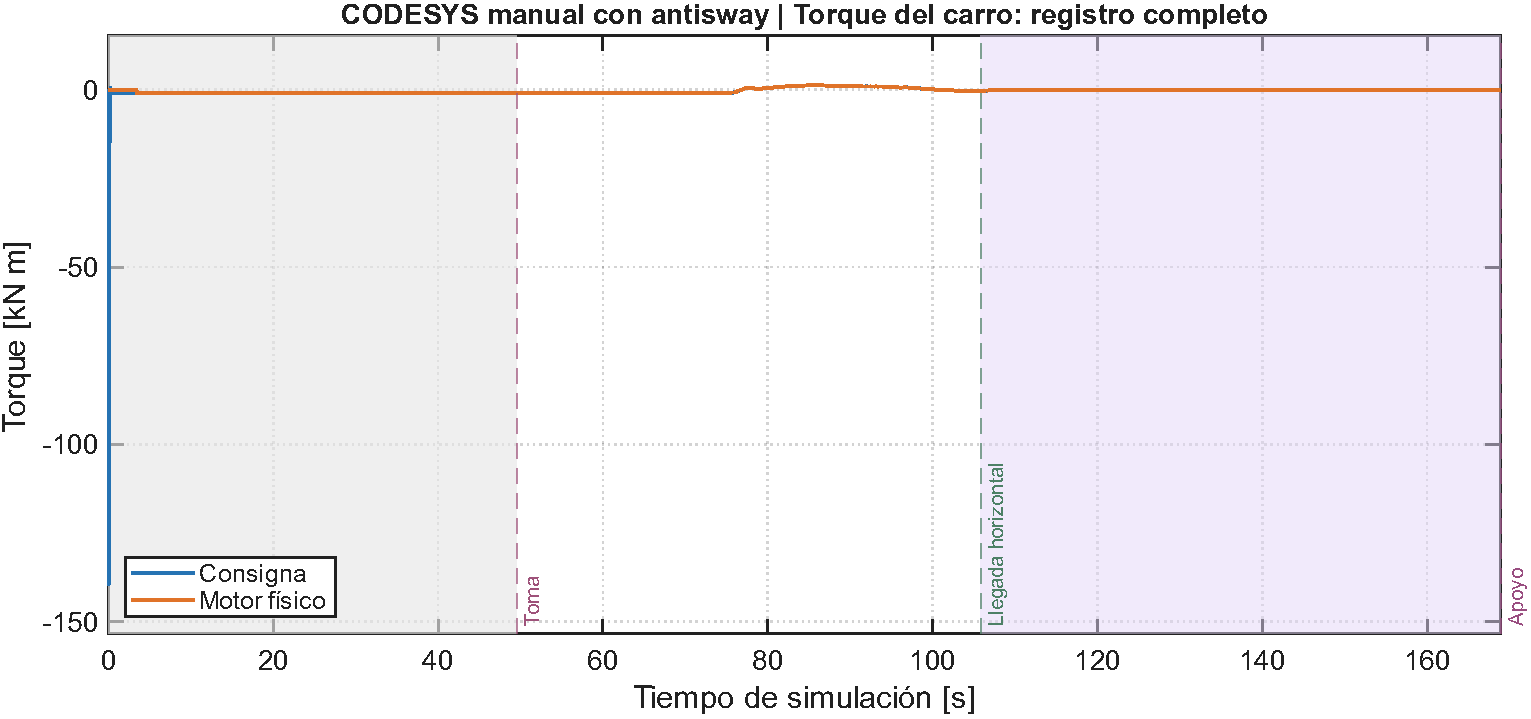
\includegraphics[width=0.98\textwidth]{graficas_individuales/manual_con_tx.pdf}
\caption{CODESYS manual con antisway: Consigna y torque físico del motor del carro en el intervalo representado, incluido el arranque.}\label{fig:individual_manual_con_tx}
\end{figure}

\begin{figure}[!htbp]
\centering
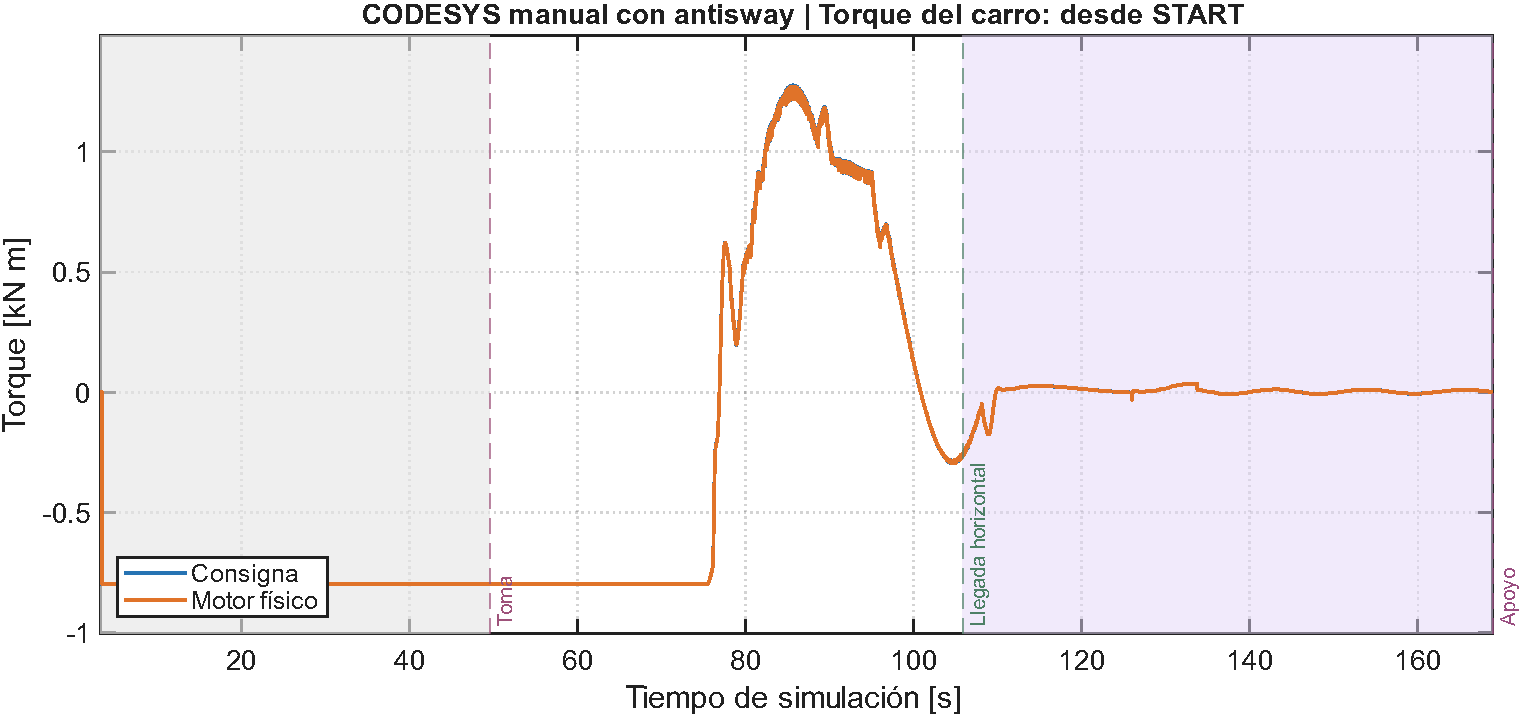
\includegraphics[width=0.98\textwidth]{graficas_individuales/manual_con_tx_zoom.pdf}
\caption{CODESYS manual con antisway: Consigna y torque físico del motor del carro desde START; la escala completa del arranque se conserva en una figura independiente.}\label{fig:individual_manual_con_tx_zoom}
\end{figure}

\begin{figure}[!htbp]
\centering
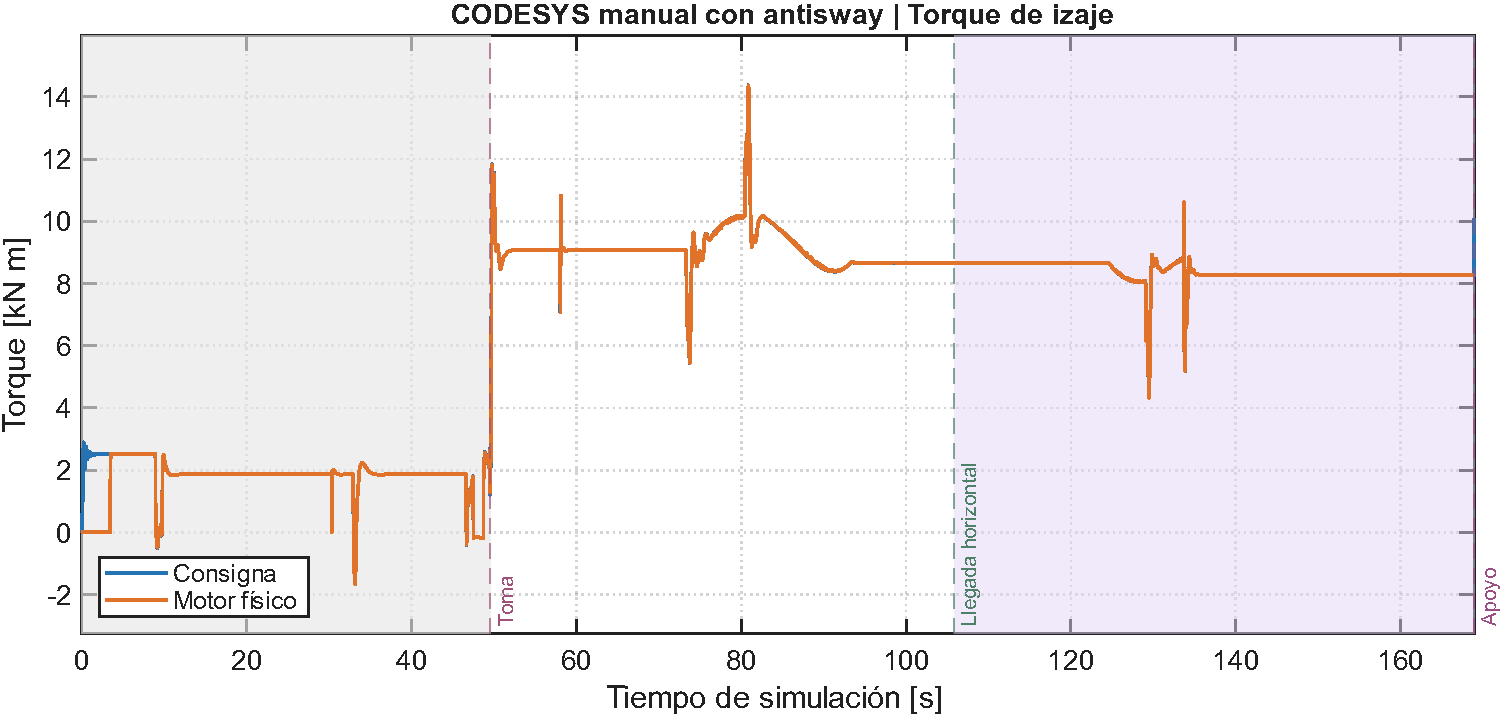
\includegraphics[width=0.98\textwidth]{graficas_individuales/manual_con_ty.pdf}
\caption{CODESYS manual con antisway: Consigna del controlador y torque físico del motor de izaje.}\label{fig:individual_manual_con_ty}
\end{figure}

\begin{figure}[!htbp]
\centering
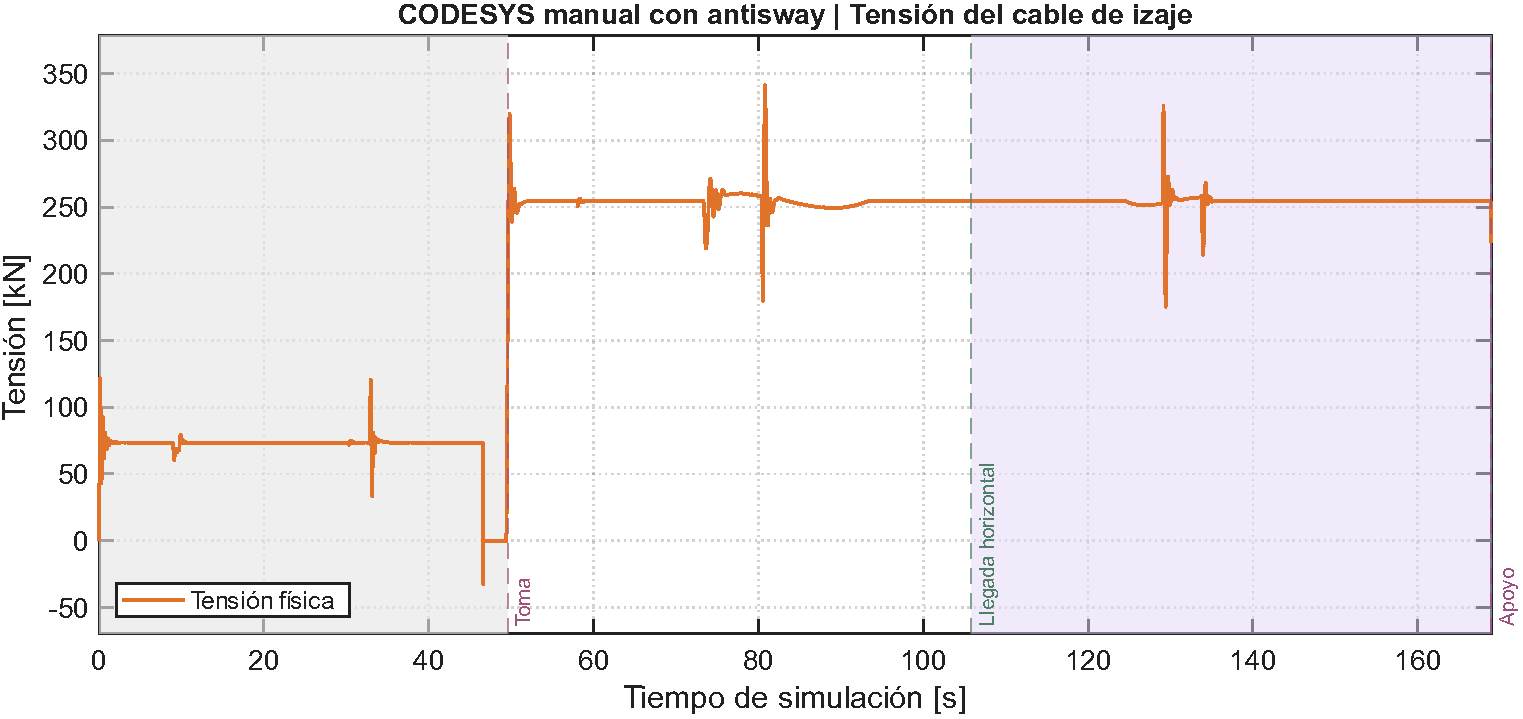
\includegraphics[width=0.98\textwidth]{graficas_individuales/manual_con_tension.pdf}
\caption{CODESYS manual con antisway: Tensión física del cable de izaje.}\label{fig:individual_manual_con_tension}
\end{figure}

\begin{figure}[!htbp]
\centering
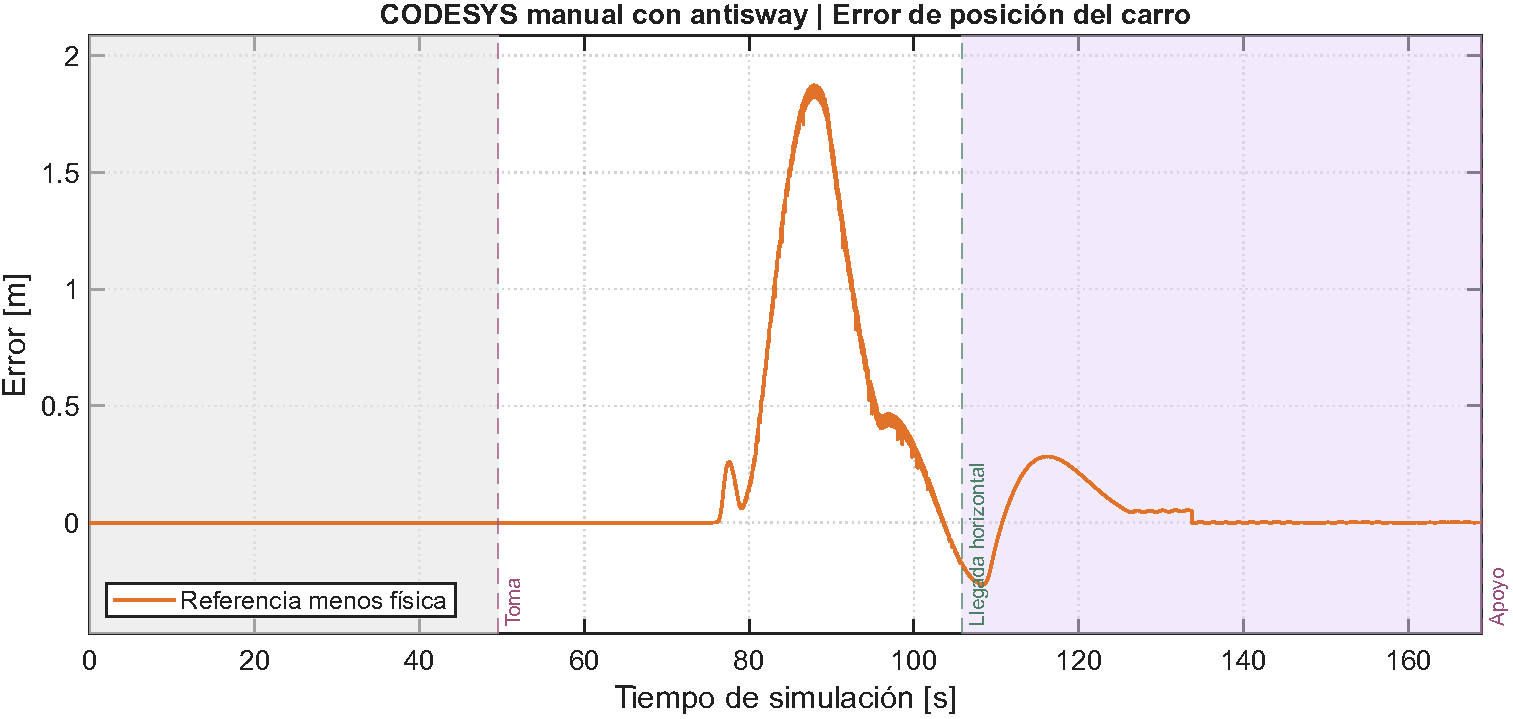
\includegraphics[width=0.98\textwidth]{graficas_individuales/manual_con_ex.pdf}
\caption{CODESYS manual con antisway: Error horizontal, calculado como referencia menos posición física.}\label{fig:individual_manual_con_ex}
\end{figure}

\begin{figure}[!htbp]
\centering
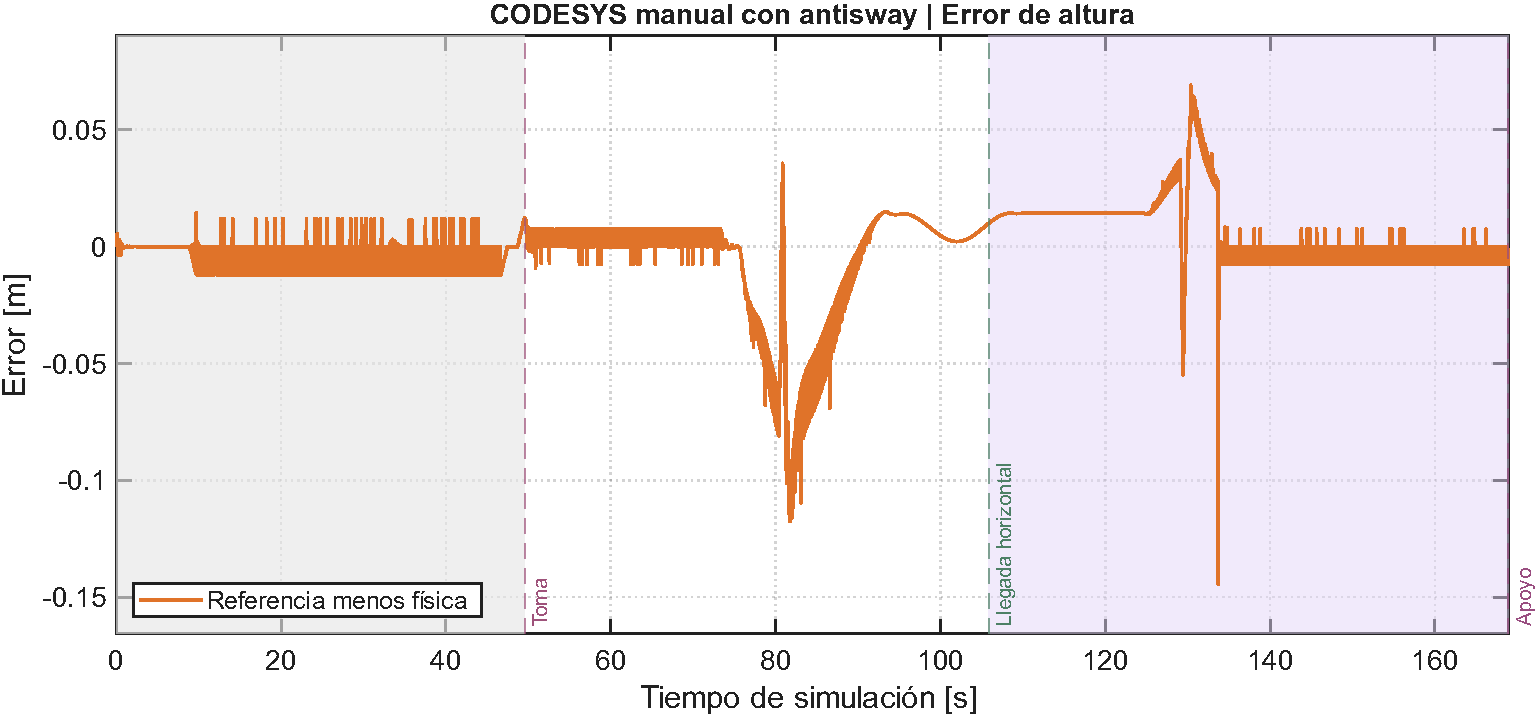
\includegraphics[width=0.98\textwidth]{graficas_individuales/manual_con_ey.pdf}
\caption{CODESYS manual con antisway: Error de altura, calculado como referencia menos altura física.}\label{fig:individual_manual_con_ey}
\end{figure}

\begin{figure}[!htbp]
\centering
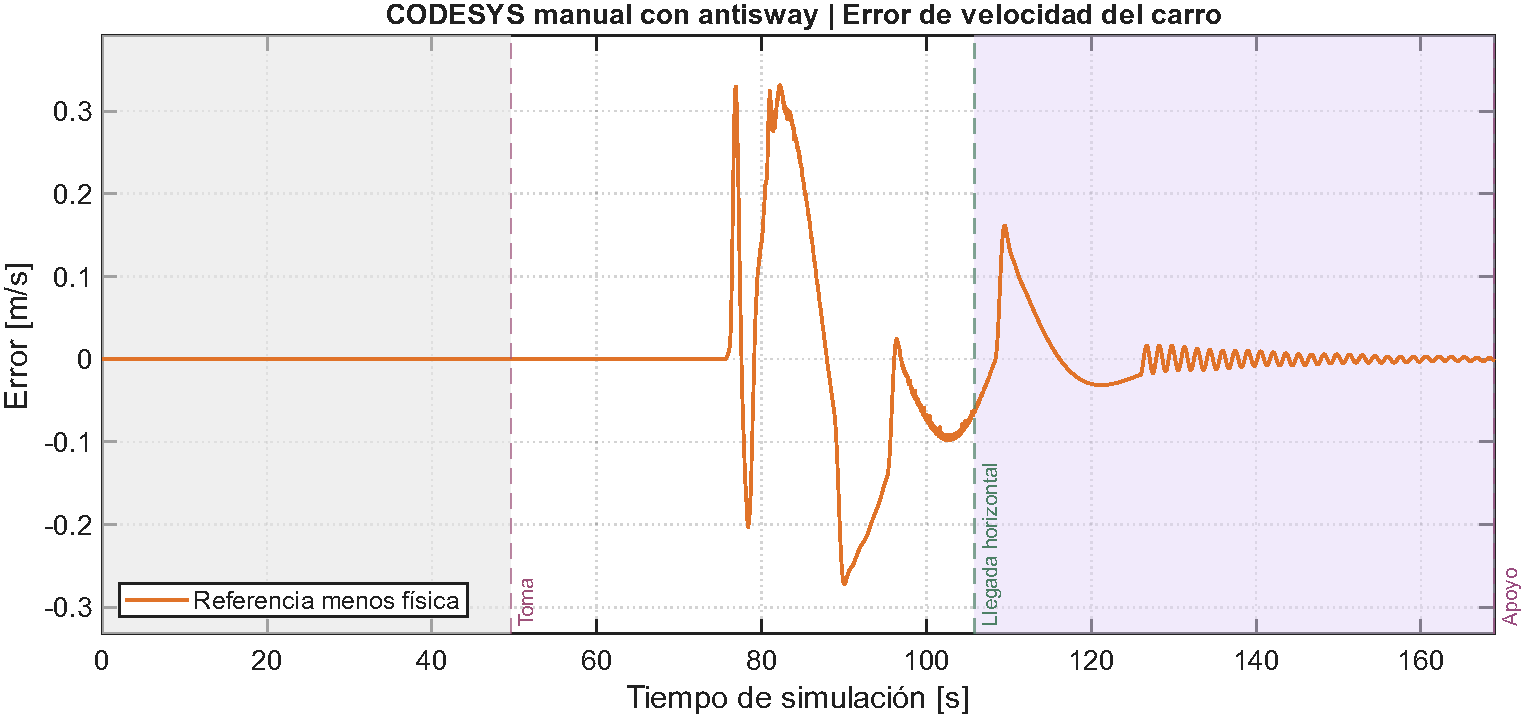
\includegraphics[width=0.98\textwidth]{graficas_individuales/manual_con_evx.pdf}
\caption{CODESYS manual con antisway: Error de velocidad del carro, calculado como referencia menos velocidad física.}\label{fig:individual_manual_con_evx}
\end{figure}

\begin{figure}[!htbp]
\centering
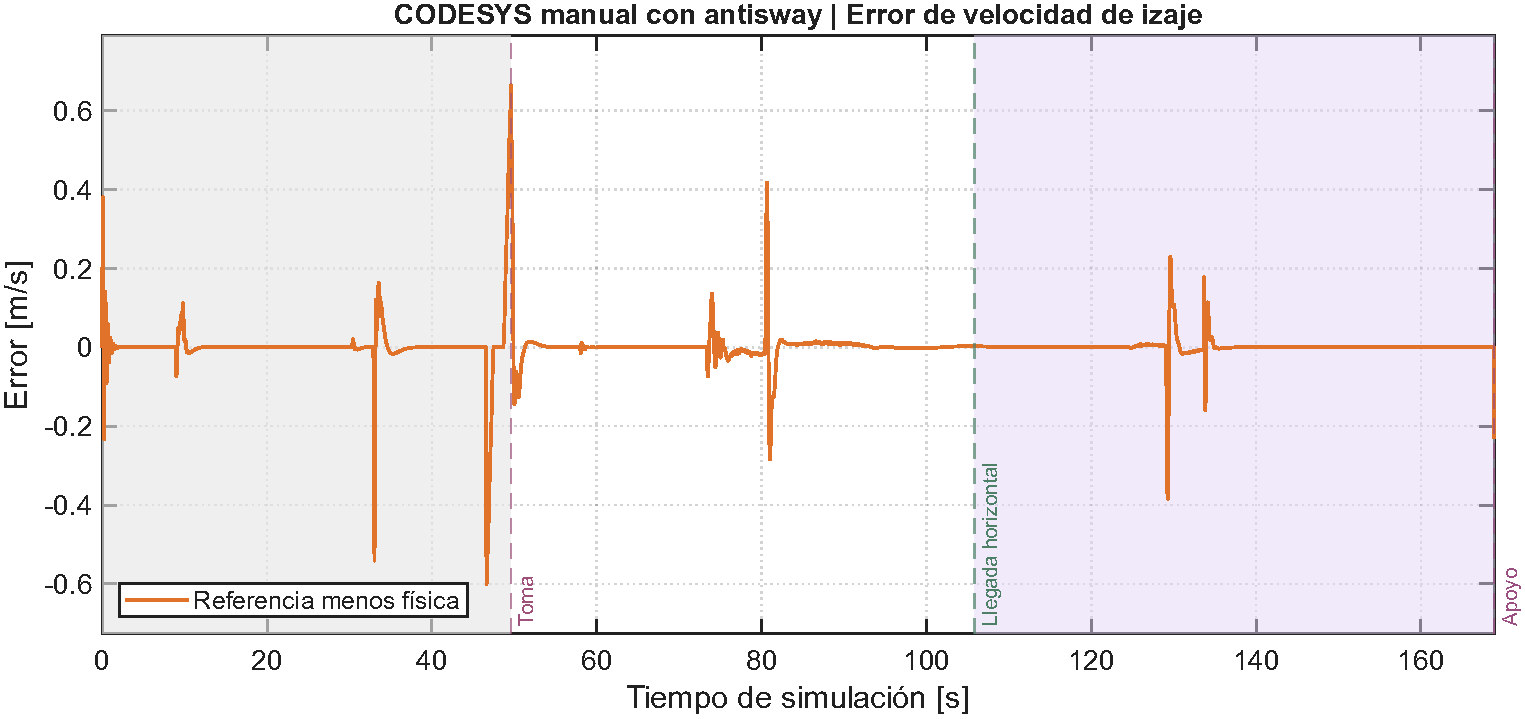
\includegraphics[width=0.98\textwidth]{graficas_individuales/manual_con_evy.pdf}
\caption{CODESYS manual con antisway: Error de velocidad de izaje, calculado como referencia menos velocidad física.}\label{fig:individual_manual_con_evy}
\end{figure}

\begin{figure}[!htbp]
\centering
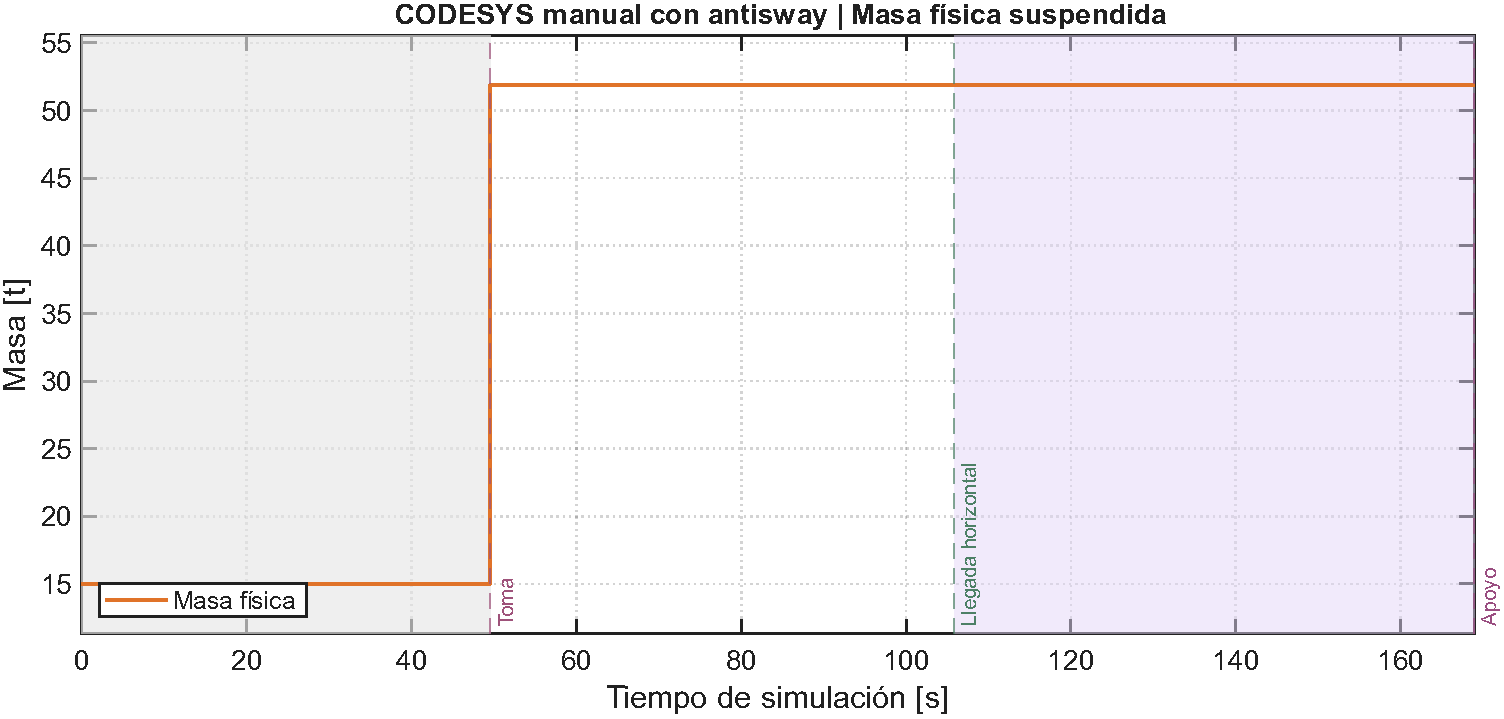
\includegraphics[width=0.98\textwidth]{graficas_individuales/manual_con_masa.pdf}
\caption{CODESYS manual con antisway: Masa física suspendida: 51,863 t representa conjunto cargado y 15 t corresponde al spreader vacío.}\label{fig:individual_manual_con_masa}
\end{figure}

\begin{figure}[!htbp]
\centering
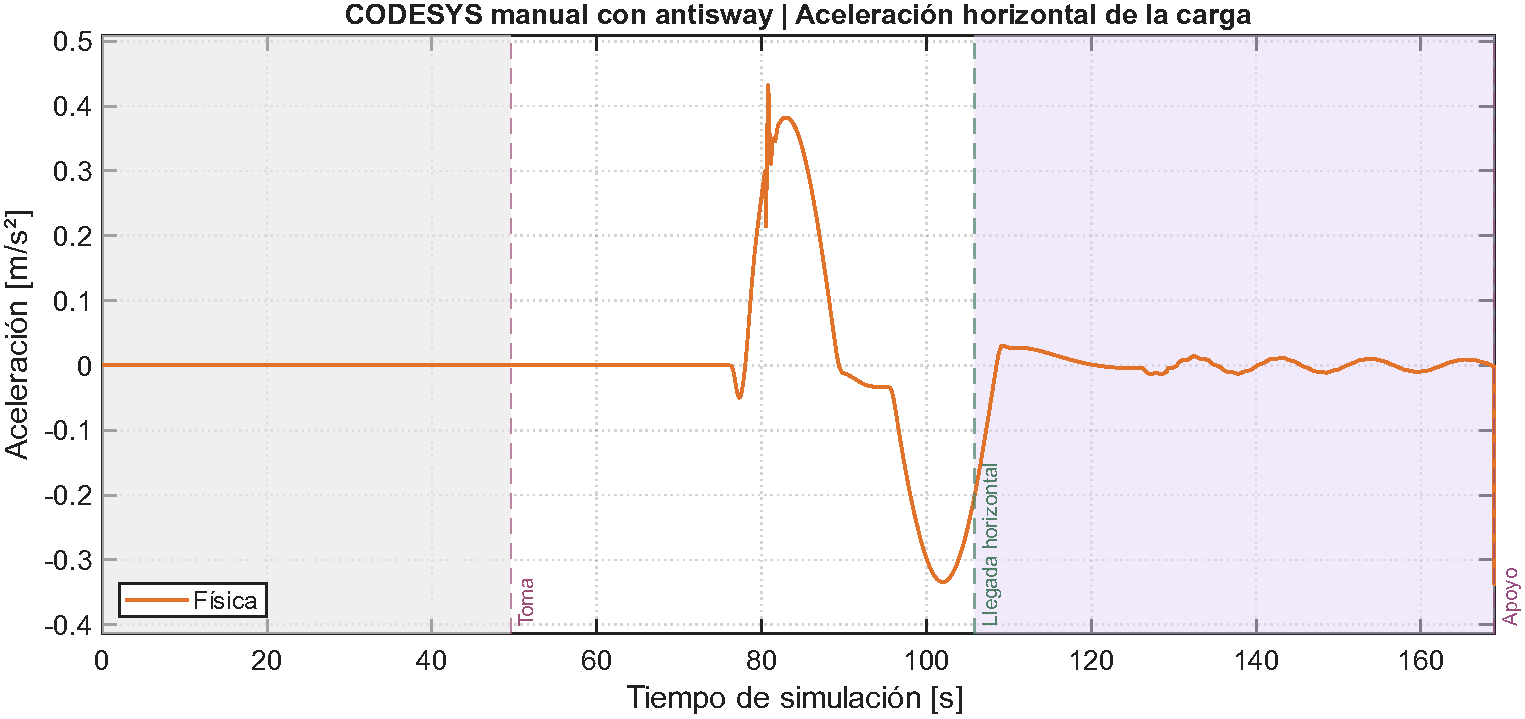
\includegraphics[width=0.98\textwidth]{graficas_individuales/manual_con_ax_carga.pdf}
\caption{CODESYS manual con antisway: Aceleración horizontal física de la carga; se conservan las oscilaciones registradas.}\label{fig:individual_manual_con_ax_carga}
\end{figure}

\clearpage
\section{Pruebas de medio ciclo con CODESYS automático}
\label{sec:ensayo_codesys_st}
\subsection{Alcance de la implementación ensayada}
Se repitió el procedimiento con supervisor y seguridad en texto estructurado generado mediante Simulink PLC Coder, con adaptadores para intercambio OPC UA, precarga del perfil y sincronización por trama. La planta, el controlador regulatorio y la HMI fueron los mismos del ensayo manual. El código generado ejecuta las máquinas de estados al recibir una nueva trama de tiempo simulado; los interbloqueos finales y la vigilancia de enlace conservan el reloj real. Esta adaptación del banco no modifica los criterios de estabilización ni fuerza la entrega física.

\subsection{CODESYS automático sin antisway: parada al límite de tres minutos}
START se solicitó a $3.24~\mathrm{s}$ y el modo manual se observó a $3.76~\mathrm{s}$. El cierre se solicitó a $46.64~\mathrm{s}$, la masa cargada se confirmó a $49.52~\mathrm{s}$ y el despegue físico a $50.00~\mathrm{s}$. Automático se solicitó a $75.28~\mathrm{s}$ y se observó a $75.36~\mathrm{s}$; la llegada horizontal fue a $105.60~\mathrm{s}$. La parada programada ocurrió exactamente a $180.00~\mathrm{s}$ sin entrega.

El carro alcanzó $22.39992~\mathrm{m}$, pero la carga permaneció a $24.07414~\mathrm{m}$ con masa $51\,863~\mathrm{kg}$. Las curvas muestran llegada horizontal y oscilación residual mientras la altura permanece en la zona de cruce. No se produjo transferencia a manual ni apoyo final. El resultado es válido para diagnóstico del control sin antisway y no aprobado como medio ciclo completo.

\begin{figure}[!htbp]
\centering
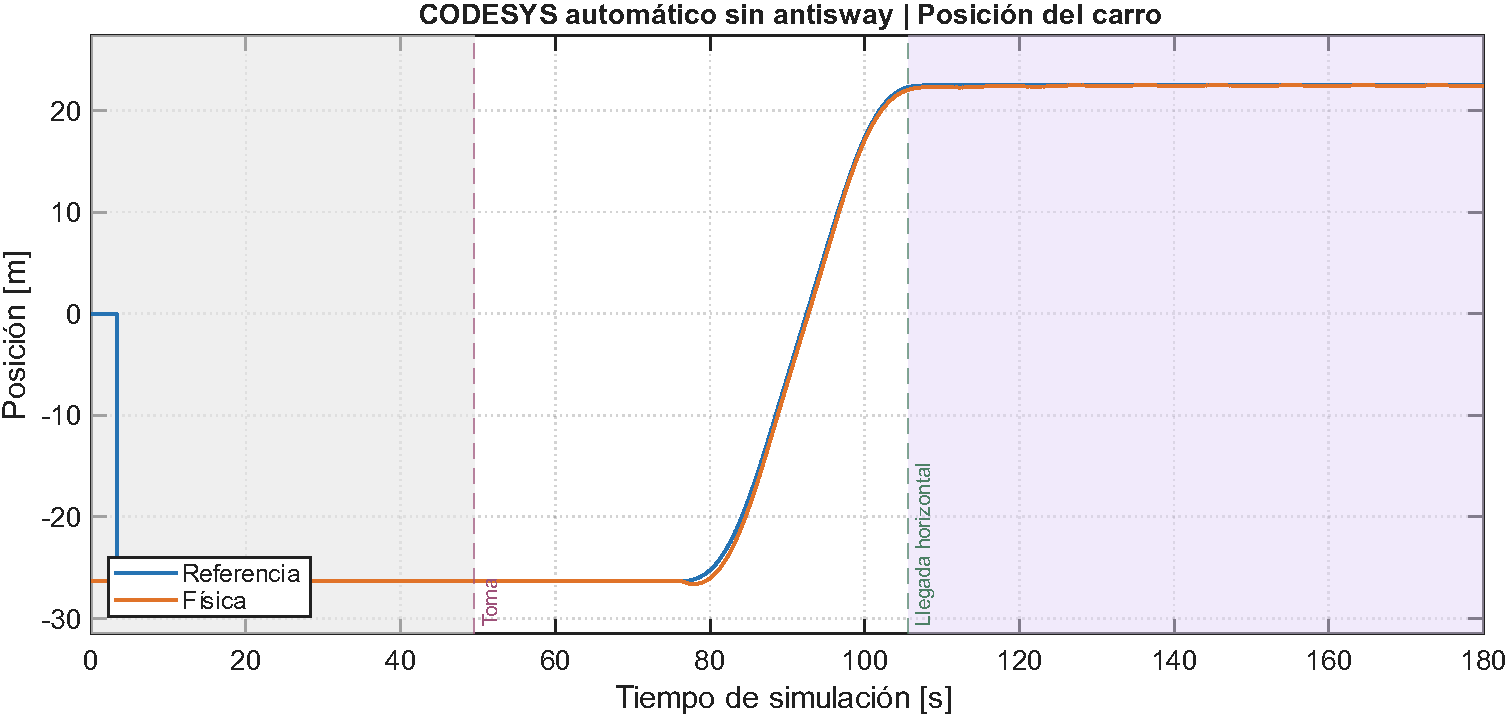
\includegraphics[width=0.98\textwidth]{graficas_individuales/automatico_sin_x.pdf}
\caption{CODESYS automático sin antisway: Posición del carro: referencia y evolución física.}\label{fig:individual_automatico_sin_x}
\end{figure}

\begin{figure}[!htbp]
\centering
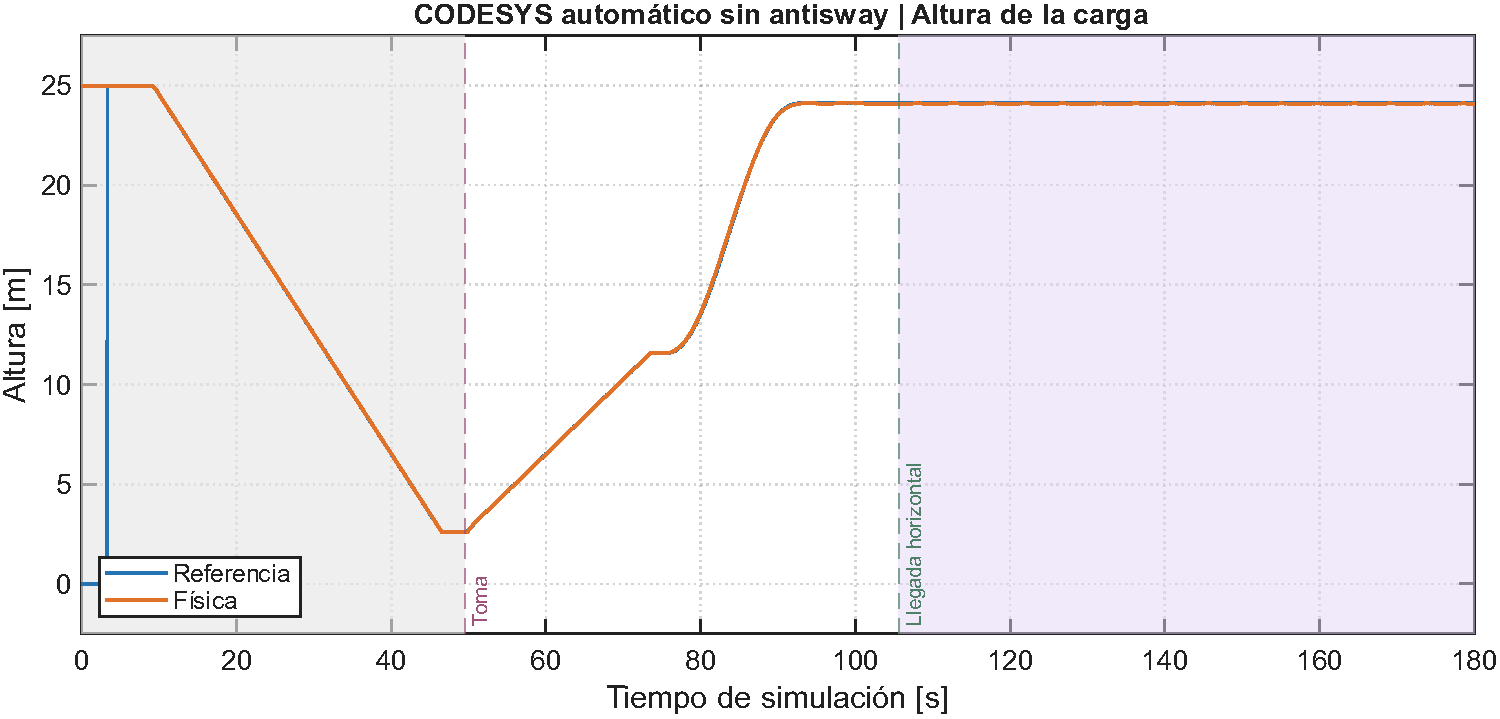
\includegraphics[width=0.98\textwidth]{graficas_individuales/automatico_sin_y.pdf}
\caption{CODESYS automático sin antisway: Altura de la carga: referencia y evolución física.}\label{fig:individual_automatico_sin_y}
\end{figure}

\begin{figure}[!htbp]
\centering
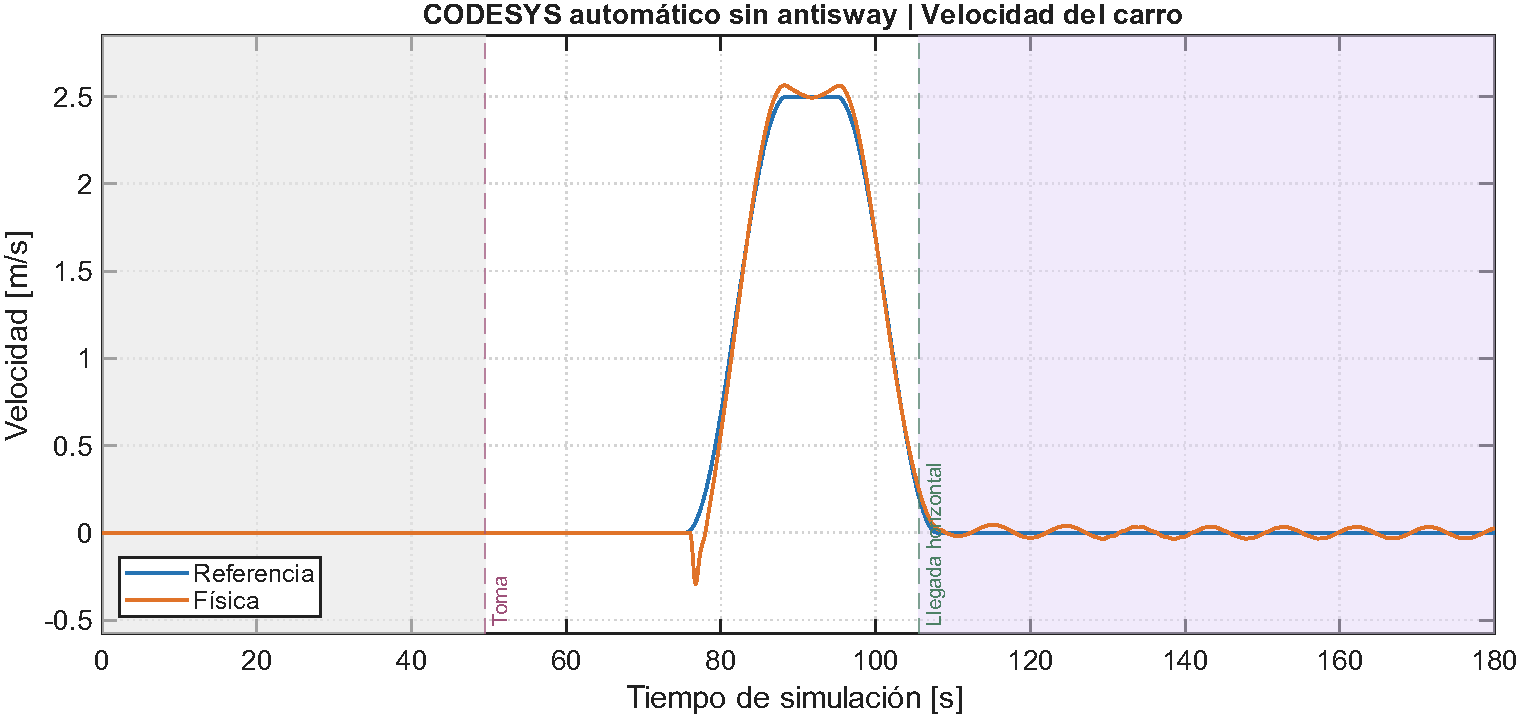
\includegraphics[width=0.98\textwidth]{graficas_individuales/automatico_sin_vx.pdf}
\caption{CODESYS automático sin antisway: Velocidad del carro: referencia y señal física.}\label{fig:individual_automatico_sin_vx}
\end{figure}

\begin{figure}[!htbp]
\centering
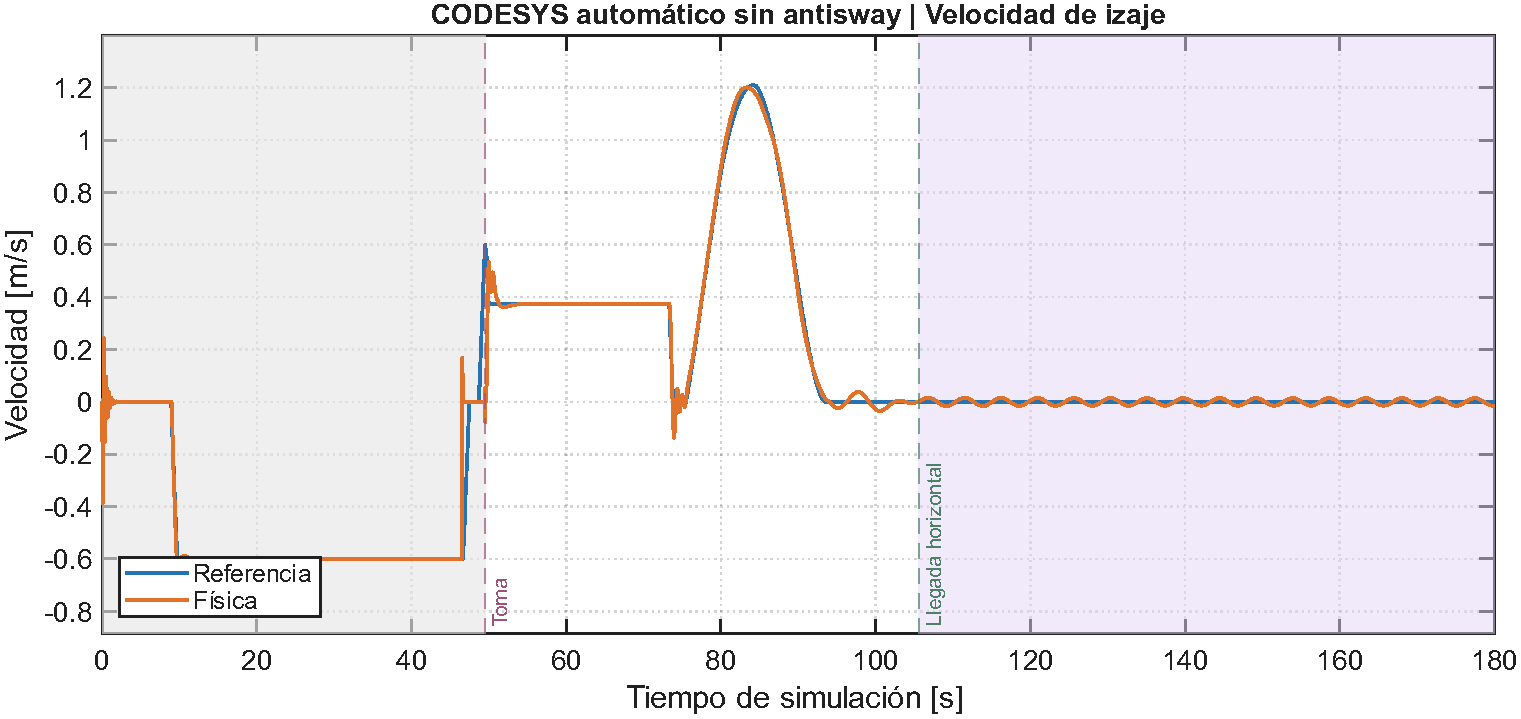
\includegraphics[width=0.98\textwidth]{graficas_individuales/automatico_sin_vy.pdf}
\caption{CODESYS automático sin antisway: Velocidad de izaje: referencia y señal física.}\label{fig:individual_automatico_sin_vy}
\end{figure}

\begin{figure}[!htbp]
\centering
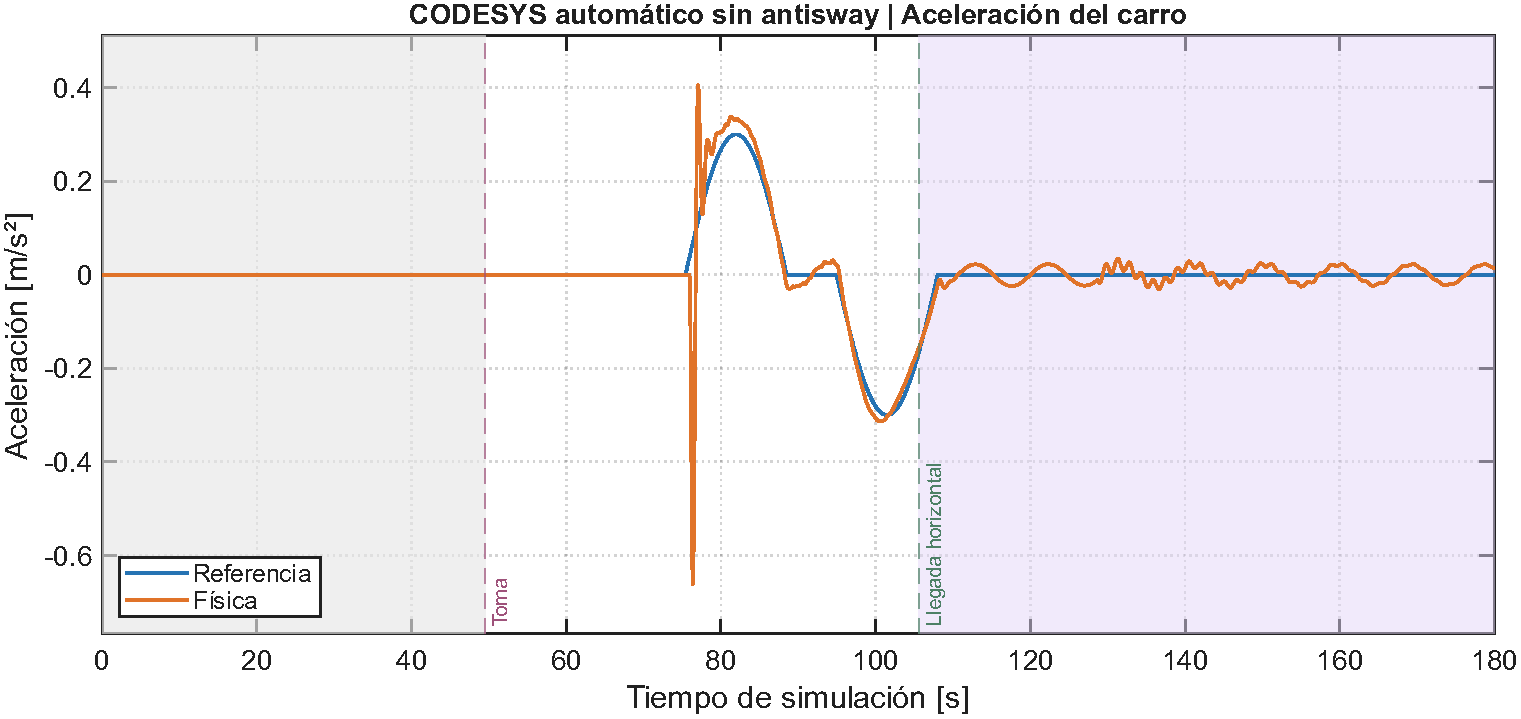
\includegraphics[width=0.98\textwidth]{graficas_individuales/automatico_sin_ax.pdf}
\caption{CODESYS automático sin antisway: Aceleración del carro: referencia y señal física.}\label{fig:individual_automatico_sin_ax}
\end{figure}

\begin{figure}[!htbp]
\centering
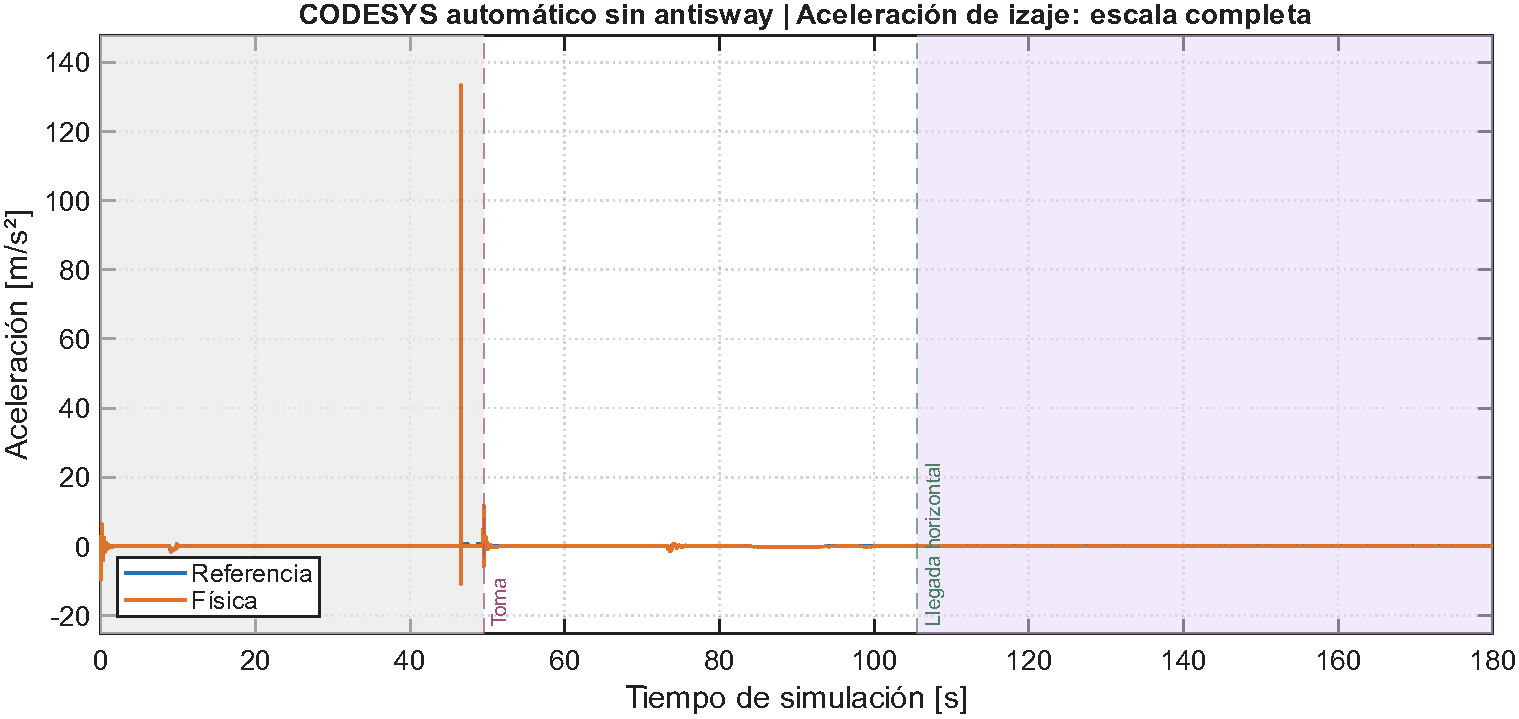
\includegraphics[width=0.98\textwidth]{graficas_individuales/automatico_sin_ay.pdf}
\caption{CODESYS automático sin antisway: Aceleración de izaje en escala completa; se conservan los picos de contacto y arranque.}\label{fig:individual_automatico_sin_ay}
\end{figure}

\begin{figure}[!htbp]
\centering
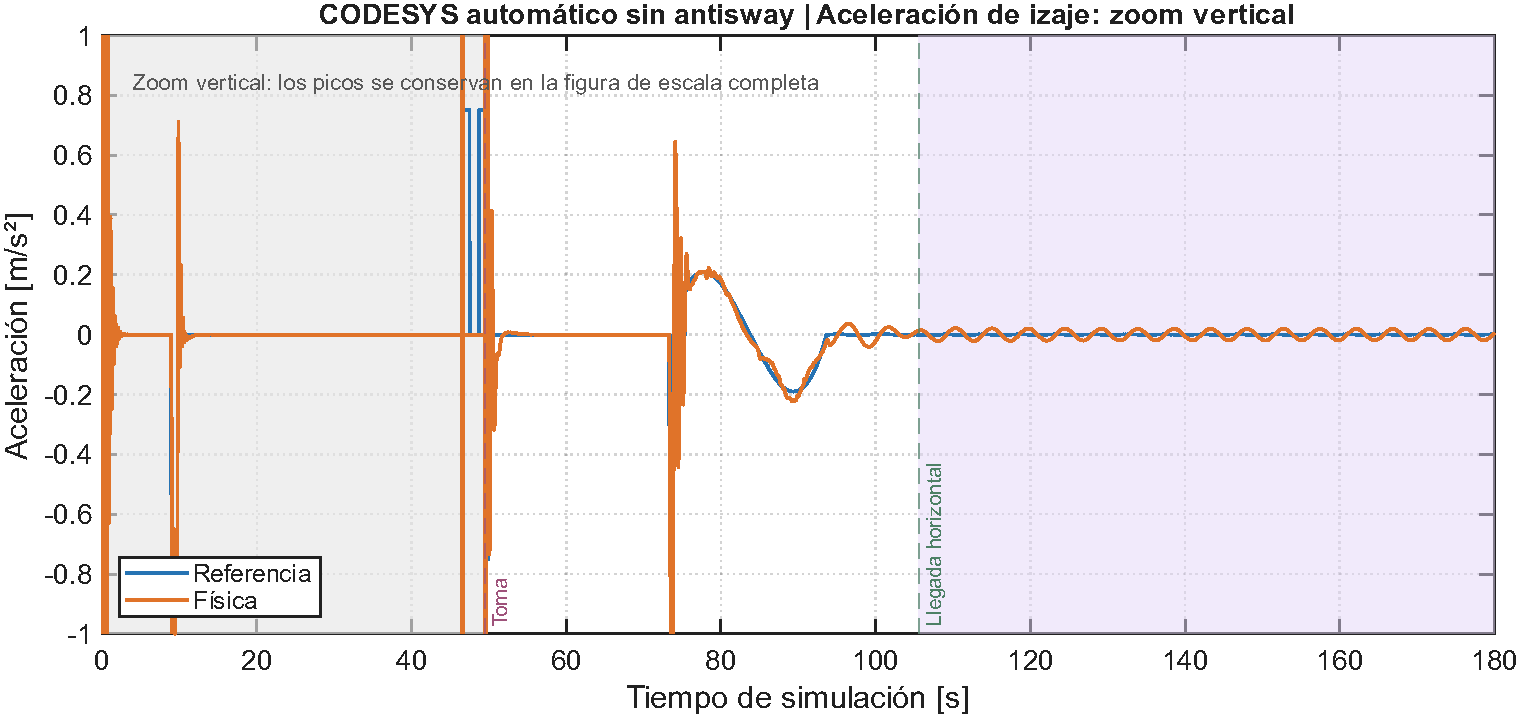
\includegraphics[width=0.98\textwidth]{graficas_individuales/automatico_sin_ay_zoom.pdf}
\caption{CODESYS automático sin antisway: Aceleración de izaje con zoom vertical entre $-1$ y $+1~\mathrm{m/s^2}$ para observar su evolución temporal. Los picos que exceden este intervalo permanecen visibles en la figura de escala completa; no se filtraron las señales.}\label{fig:individual_automatico_sin_ay_zoom}
\end{figure}

\begin{figure}[!htbp]
\centering
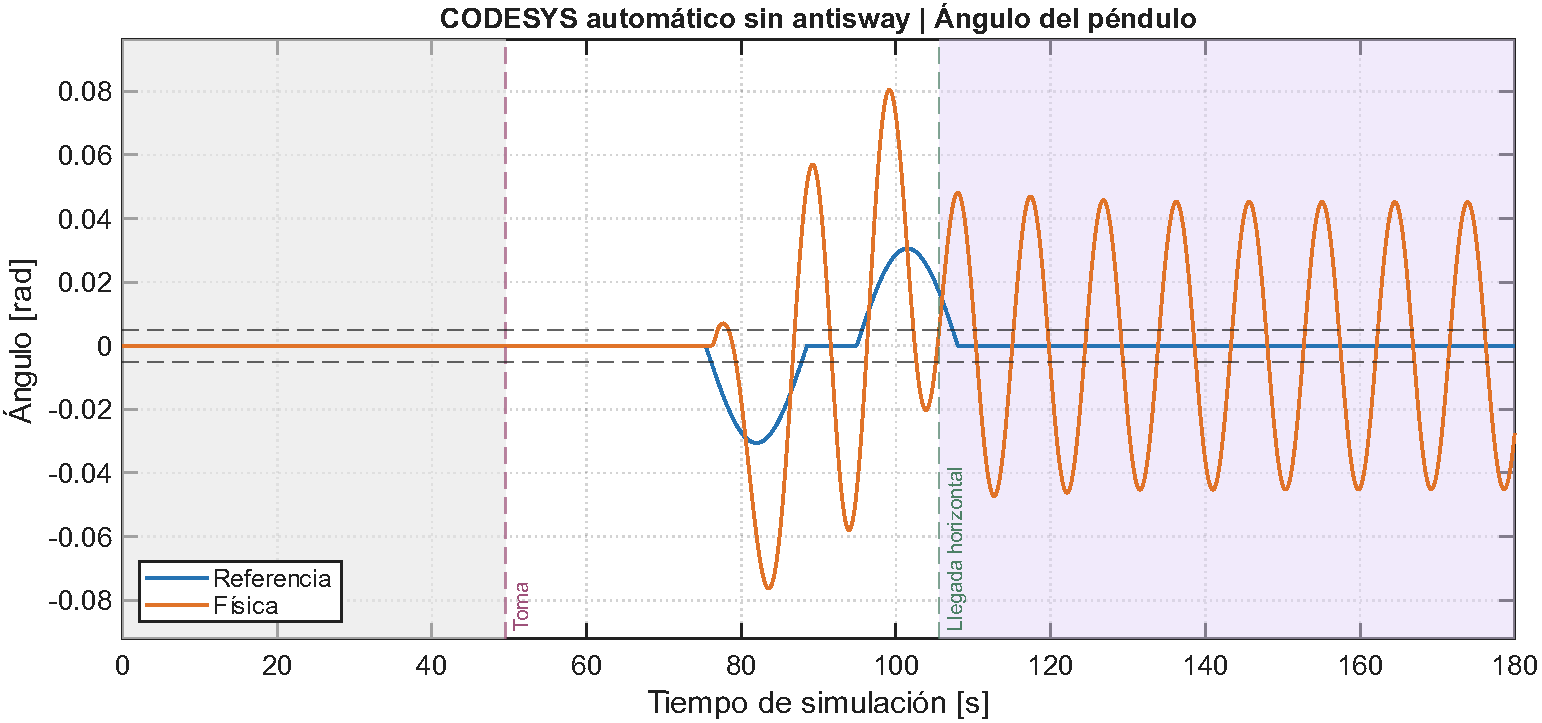
\includegraphics[width=0.98\textwidth]{graficas_individuales/automatico_sin_theta.pdf}
\caption{CODESYS automático sin antisway: Ángulo físico y de referencia del péndulo. Las líneas horizontales señalan los umbrales angulares del descenso.}\label{fig:individual_automatico_sin_theta}
\end{figure}

\begin{figure}[!htbp]
\centering
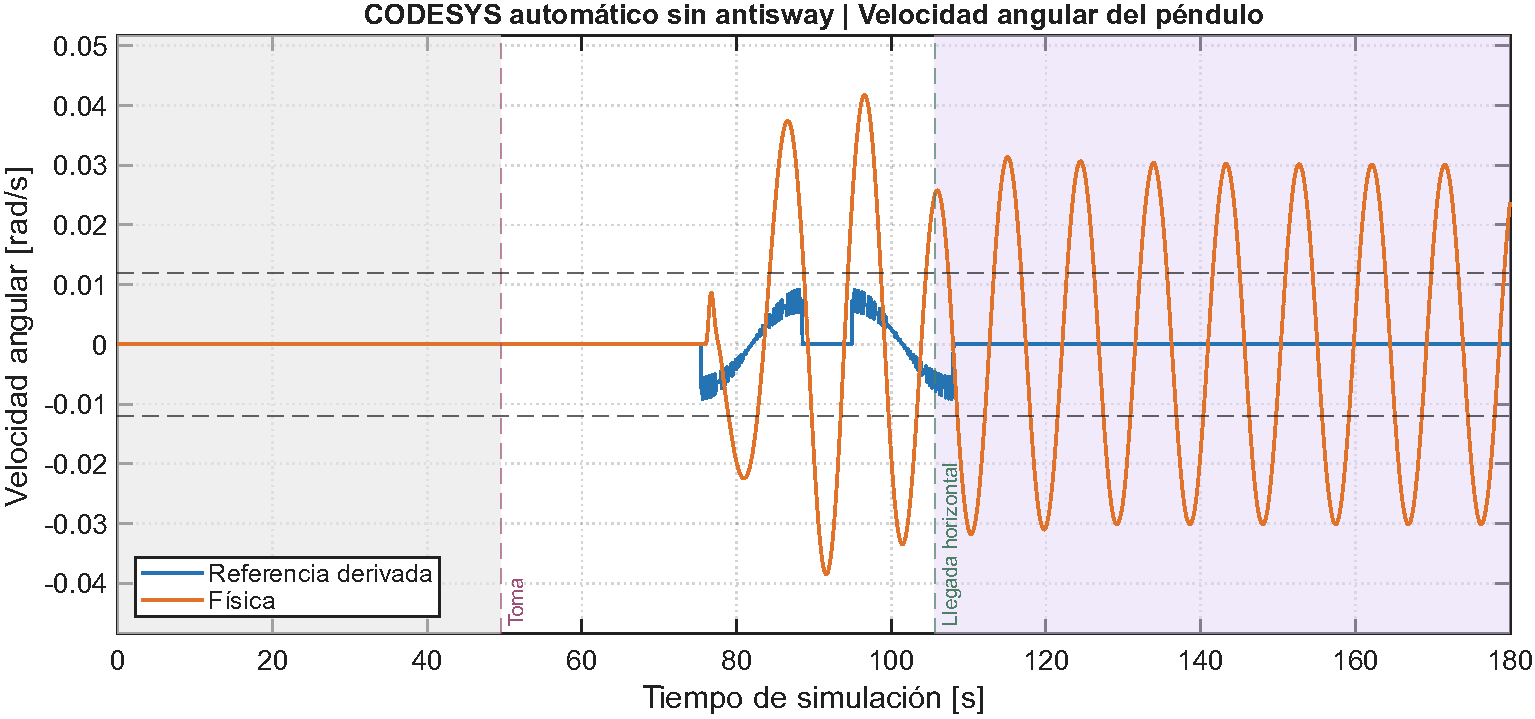
\includegraphics[width=0.98\textwidth]{graficas_individuales/automatico_sin_omega.pdf}
\caption{CODESYS automático sin antisway: Velocidad angular física y referencia derivada numéricamente; se distinguen ambas fuentes. Las líneas horizontales indican los umbrales del descenso.}\label{fig:individual_automatico_sin_omega}
\end{figure}

\begin{figure}[!htbp]
\centering
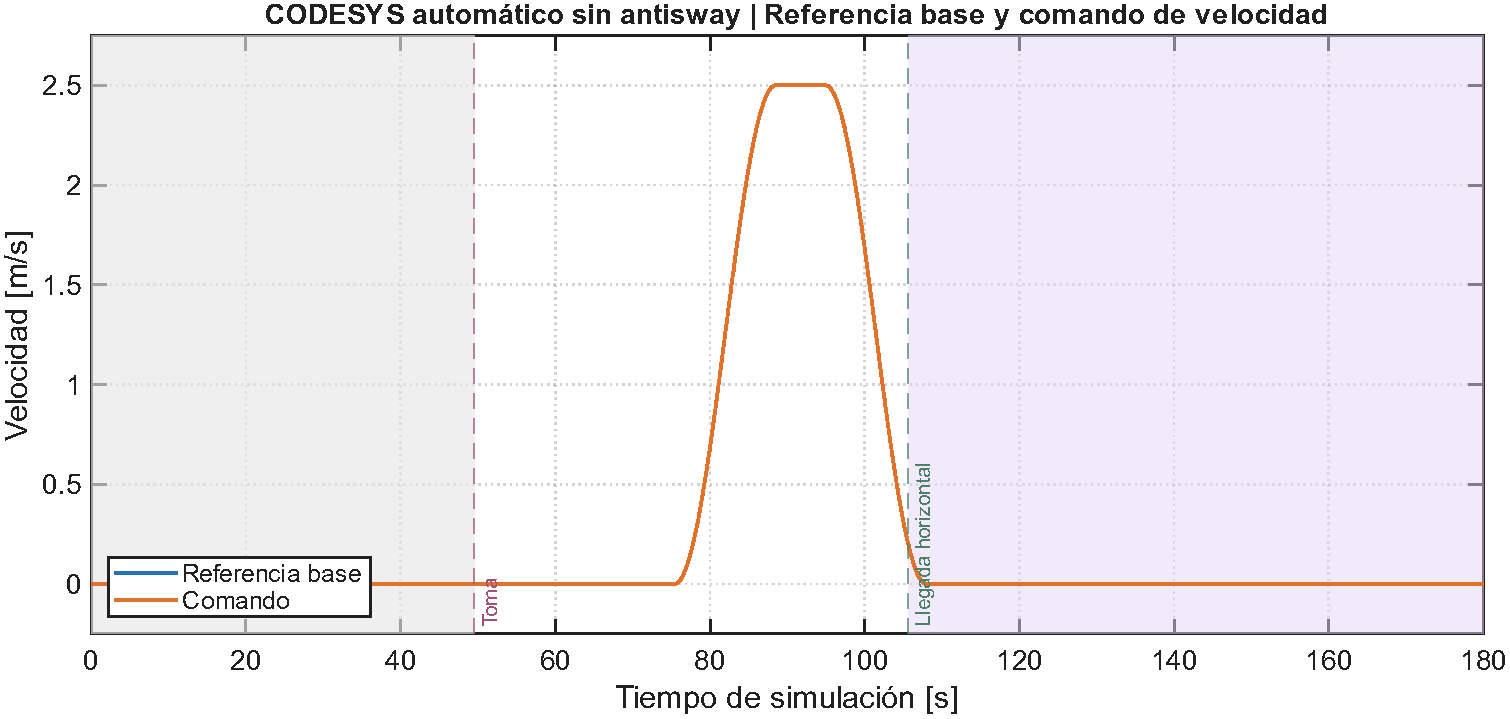
\includegraphics[width=0.98\textwidth]{graficas_individuales/automatico_sin_vcmd.pdf}
\caption{CODESYS automático sin antisway: Referencia base y comando de velocidad; su diferencia corresponde a la contribución antisway efectiva en el sumador.}\label{fig:individual_automatico_sin_vcmd}
\end{figure}

\begin{figure}[!htbp]
\centering
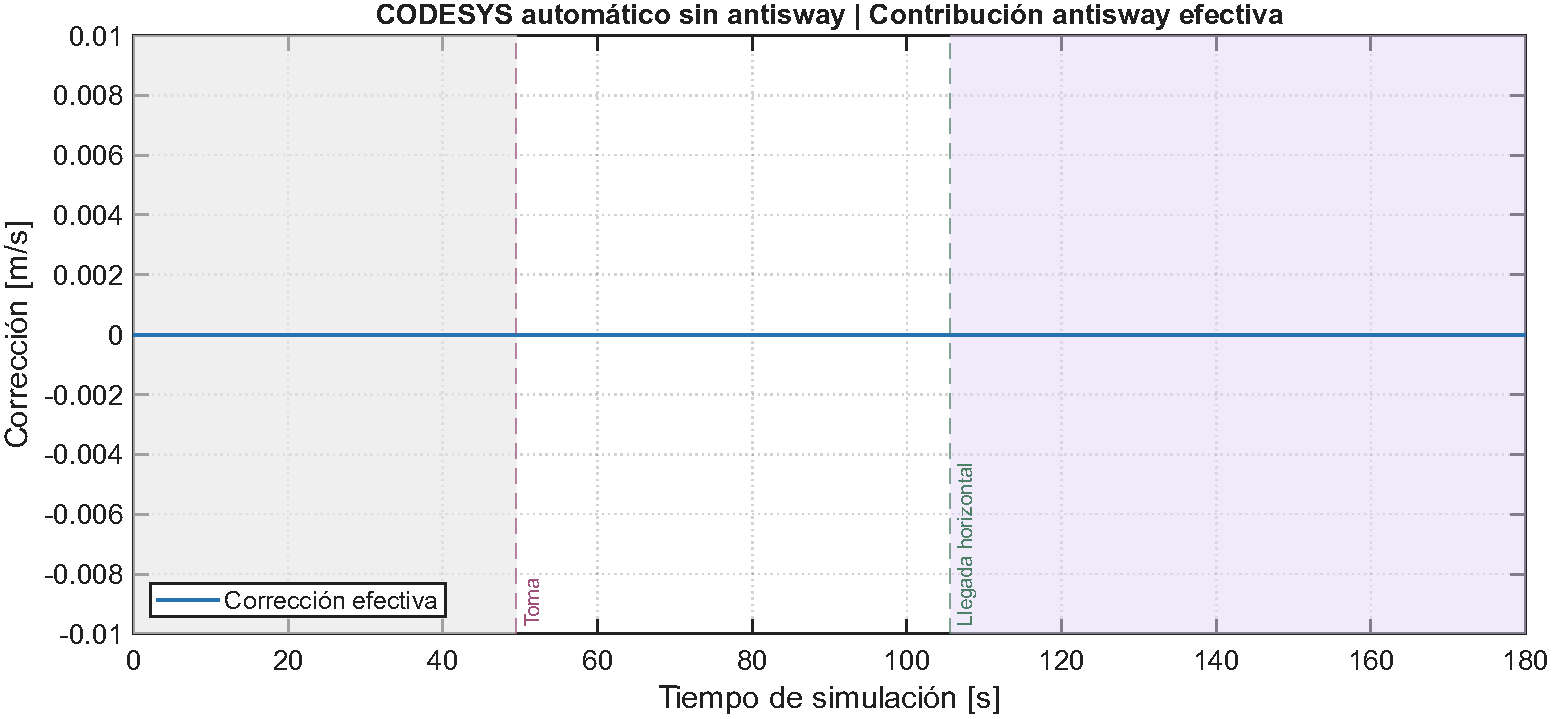
\includegraphics[width=0.98\textwidth]{graficas_individuales/automatico_sin_sw.pdf}
\caption{CODESYS automático sin antisway: Contribución antisway efectivamente sumada al comando de velocidad.}\label{fig:individual_automatico_sin_sw}
\end{figure}

La verificación nativa confirmó corrección efectiva cero y comando igual a referencia en las $180\,001$ muestras del controlador. El registro completo permite observar los torques, aceleraciones y tensión hasta la parada, sin el faltante de la variante manual sin antisway. La masa física no cae a la del spreader y el perfil del destino no aumenta. La indicación de antisway habilitado en la HMI corresponde a permiso de ejecución; la ganancia experimental cero impide su contribución al comando.

\begin{figure}[!htbp]
\centering
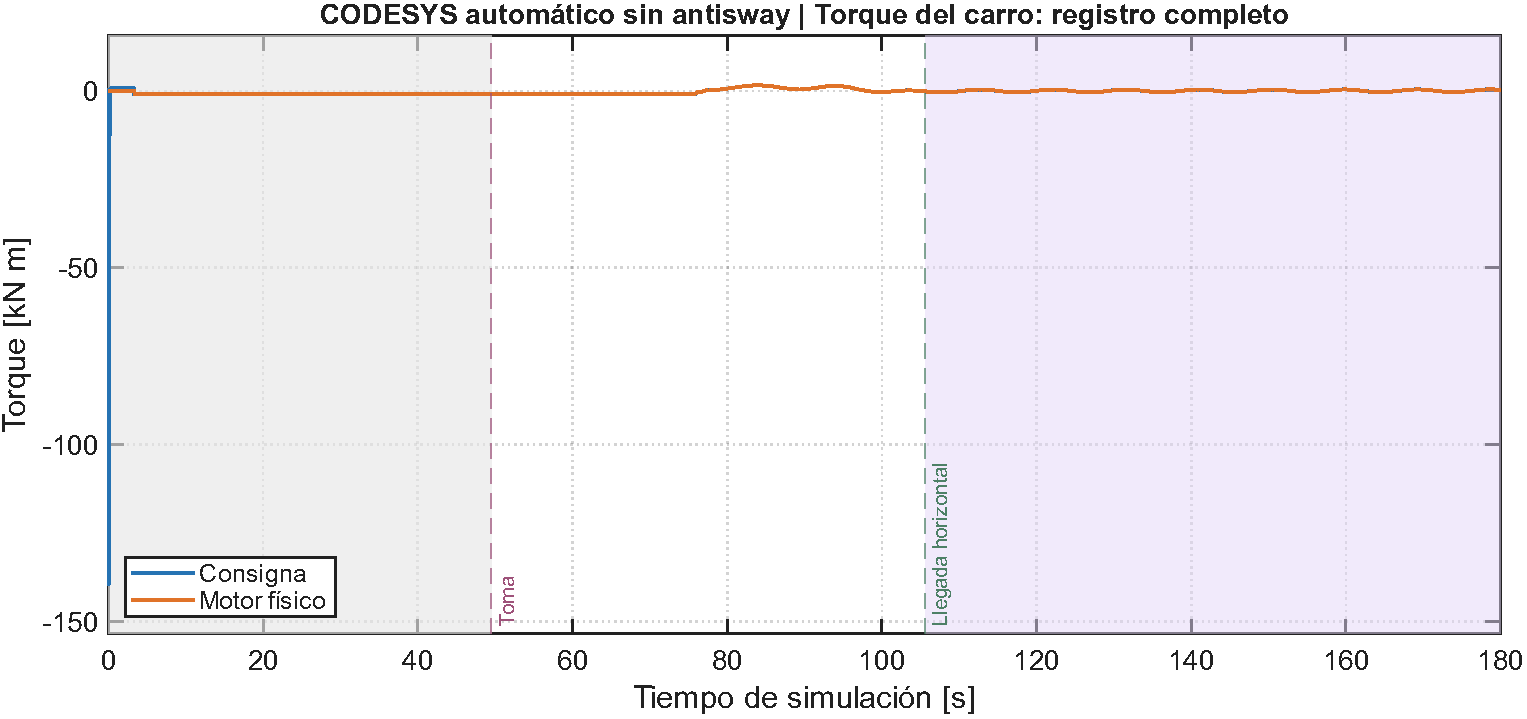
\includegraphics[width=0.98\textwidth]{graficas_individuales/automatico_sin_tx.pdf}
\caption{CODESYS automático sin antisway: Consigna y torque físico del motor del carro en el intervalo representado, incluido el arranque.}\label{fig:individual_automatico_sin_tx}
\end{figure}

\begin{figure}[!htbp]
\centering
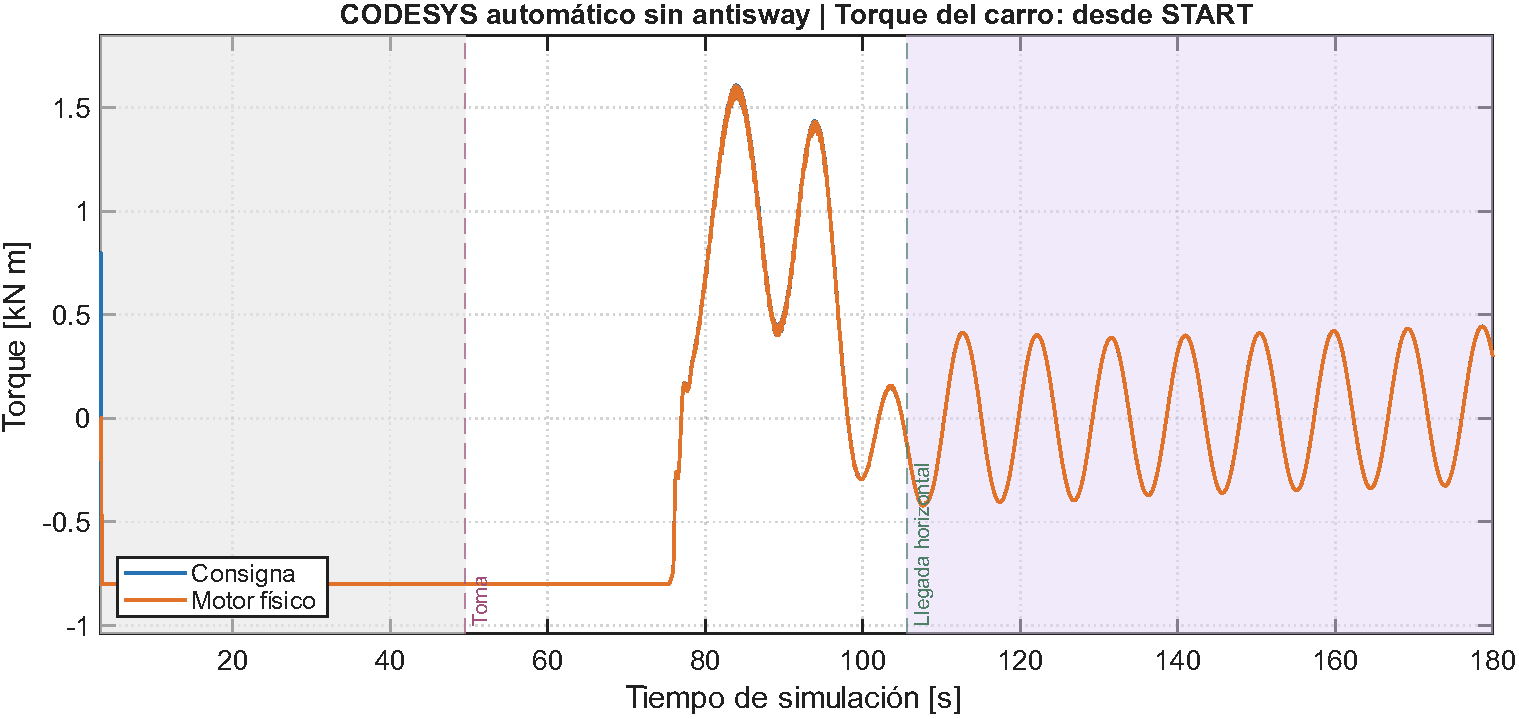
\includegraphics[width=0.98\textwidth]{graficas_individuales/automatico_sin_tx_zoom.pdf}
\caption{CODESYS automático sin antisway: Consigna y torque físico del motor del carro desde START; la escala completa del arranque se conserva en una figura independiente.}\label{fig:individual_automatico_sin_tx_zoom}
\end{figure}

\begin{figure}[!htbp]
\centering
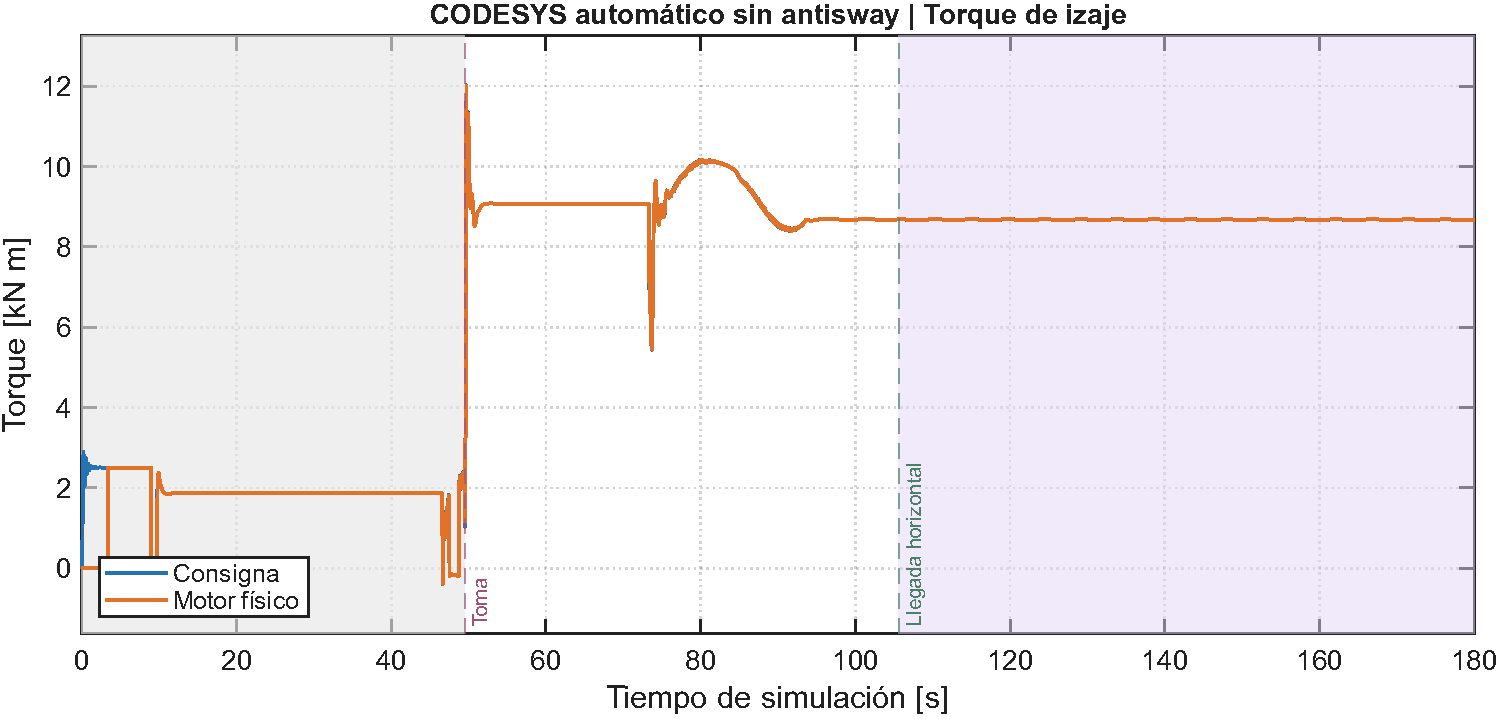
\includegraphics[width=0.98\textwidth]{graficas_individuales/automatico_sin_ty.pdf}
\caption{CODESYS automático sin antisway: Consigna del controlador y torque físico del motor de izaje.}\label{fig:individual_automatico_sin_ty}
\end{figure}

\begin{figure}[!htbp]
\centering
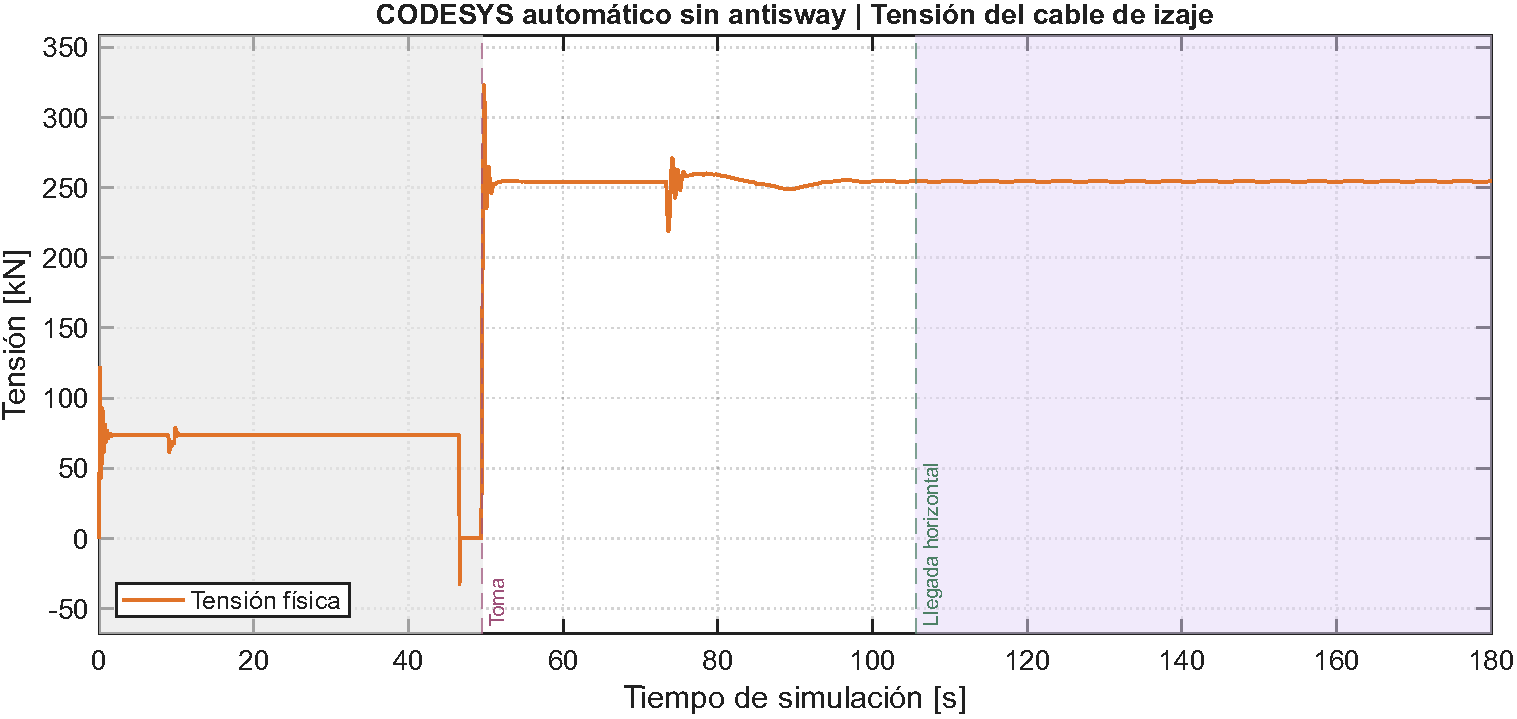
\includegraphics[width=0.98\textwidth]{graficas_individuales/automatico_sin_tension.pdf}
\caption{CODESYS automático sin antisway: Tensión física del cable de izaje.}\label{fig:individual_automatico_sin_tension}
\end{figure}

\begin{figure}[!htbp]
\centering
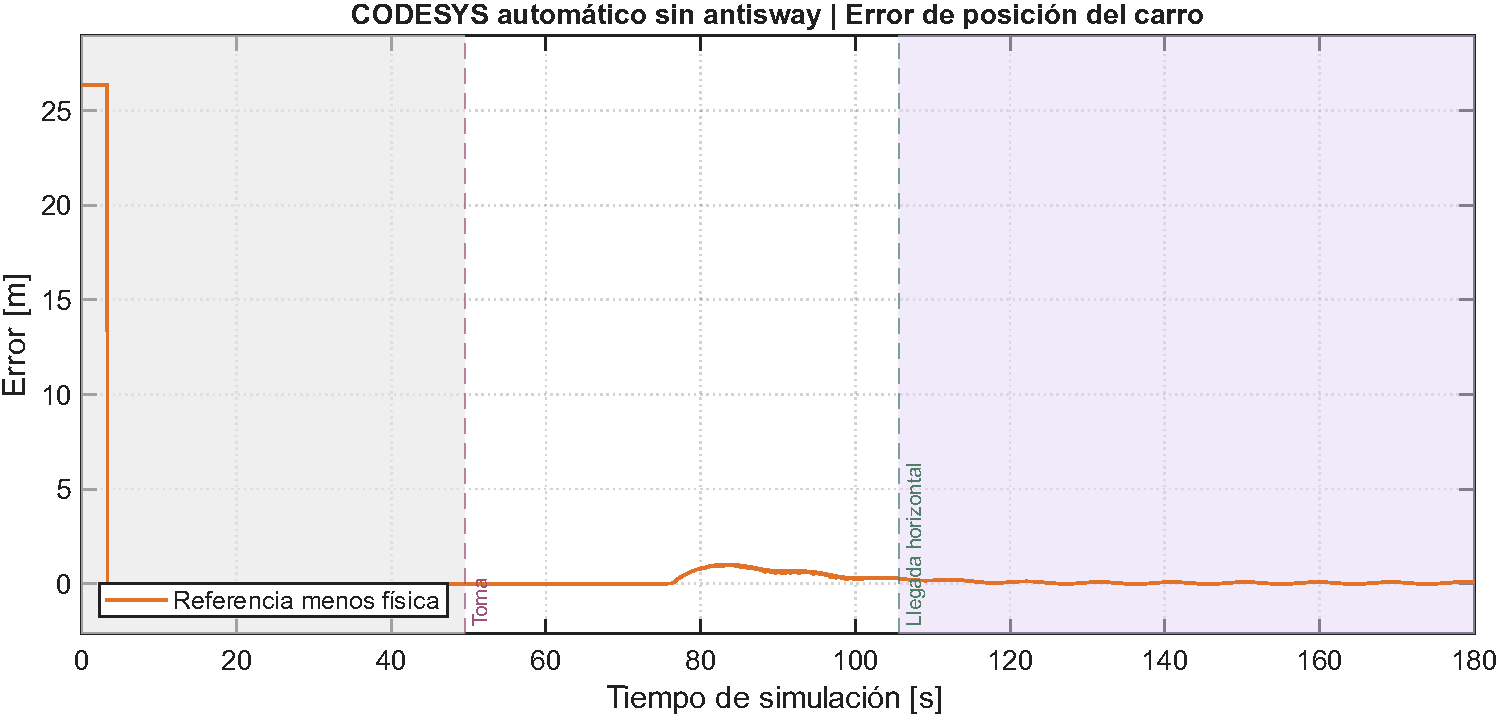
\includegraphics[width=0.98\textwidth]{graficas_individuales/automatico_sin_ex.pdf}
\caption{CODESYS automático sin antisway: Error horizontal, calculado como referencia menos posición física.}\label{fig:individual_automatico_sin_ex}
\end{figure}

\begin{figure}[!htbp]
\centering
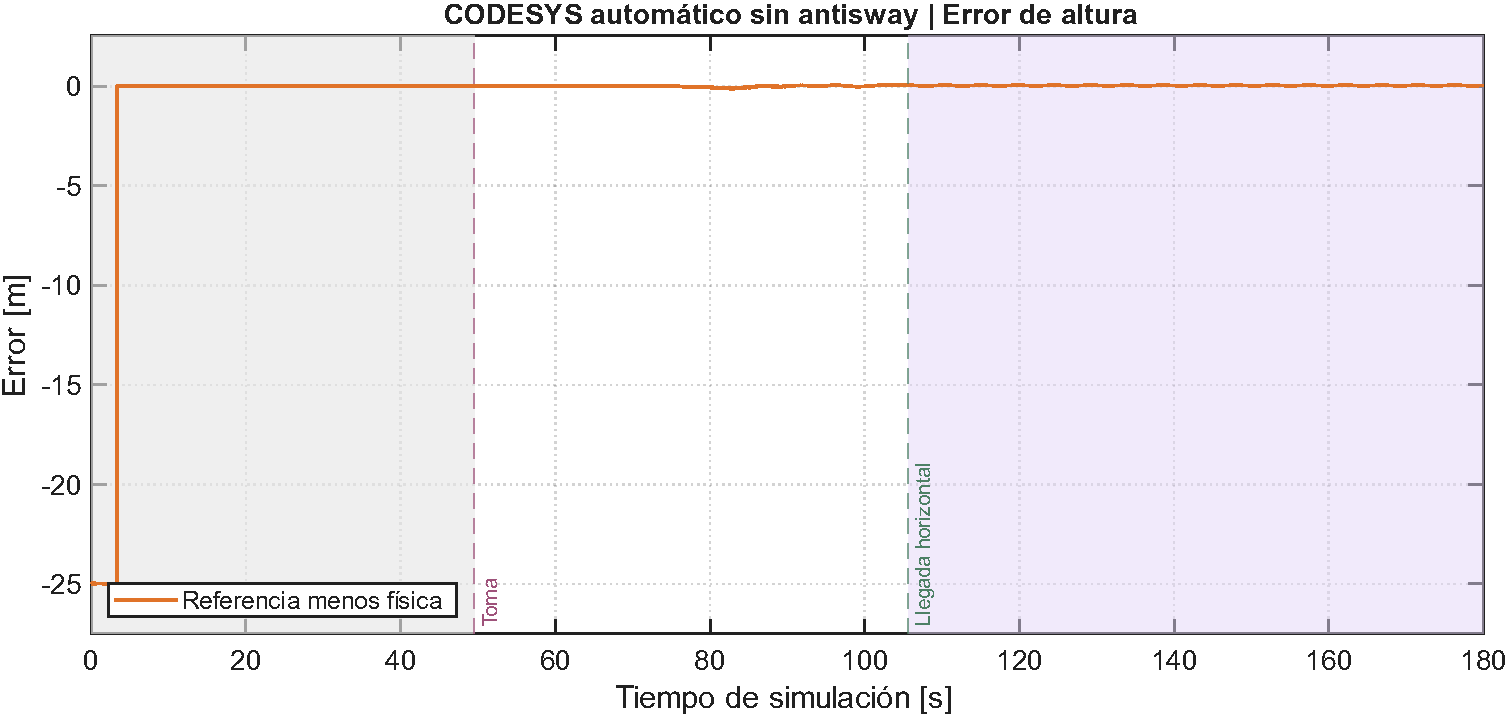
\includegraphics[width=0.98\textwidth]{graficas_individuales/automatico_sin_ey.pdf}
\caption{CODESYS automático sin antisway: Error de altura, calculado como referencia menos altura física.}\label{fig:individual_automatico_sin_ey}
\end{figure}

\begin{figure}[!htbp]
\centering
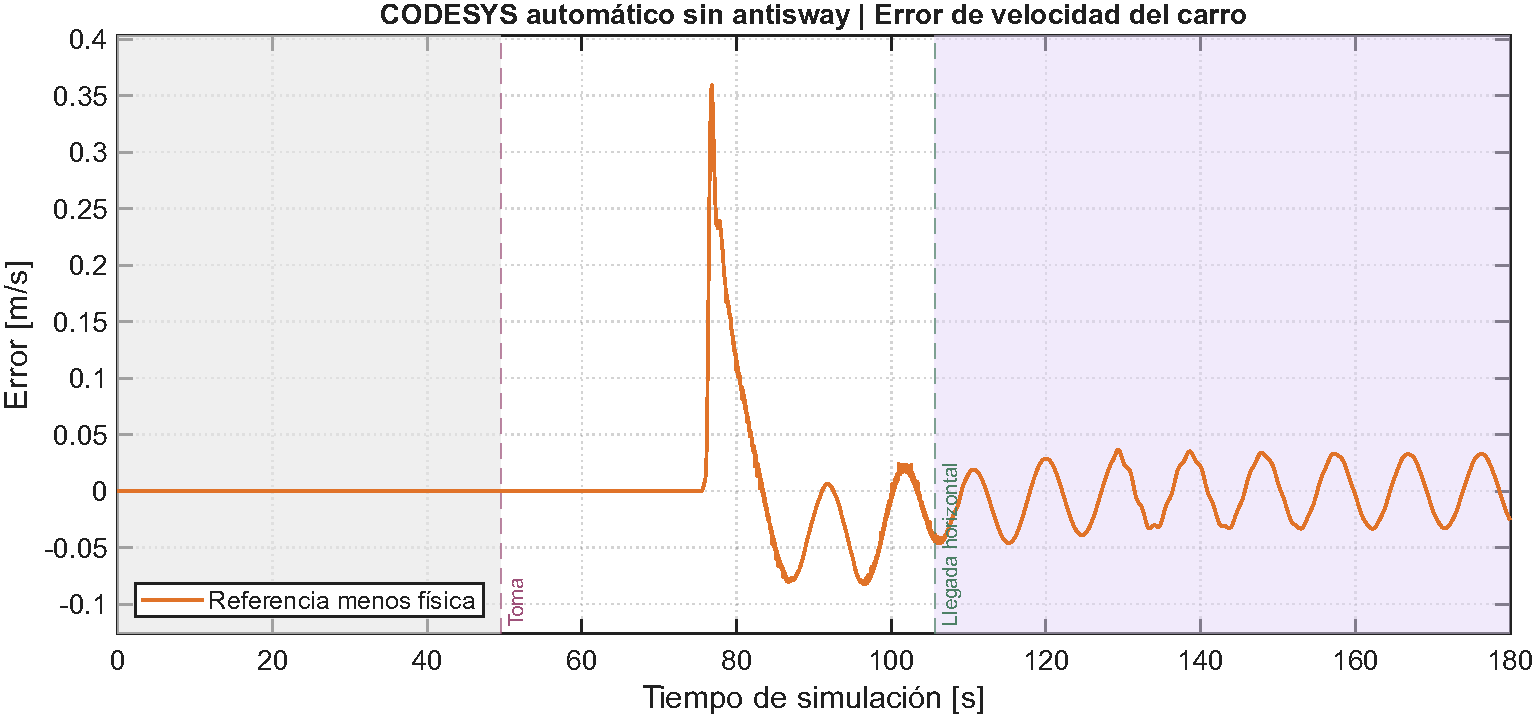
\includegraphics[width=0.98\textwidth]{graficas_individuales/automatico_sin_evx.pdf}
\caption{CODESYS automático sin antisway: Error de velocidad del carro, calculado como referencia menos velocidad física.}\label{fig:individual_automatico_sin_evx}
\end{figure}

\begin{figure}[!htbp]
\centering
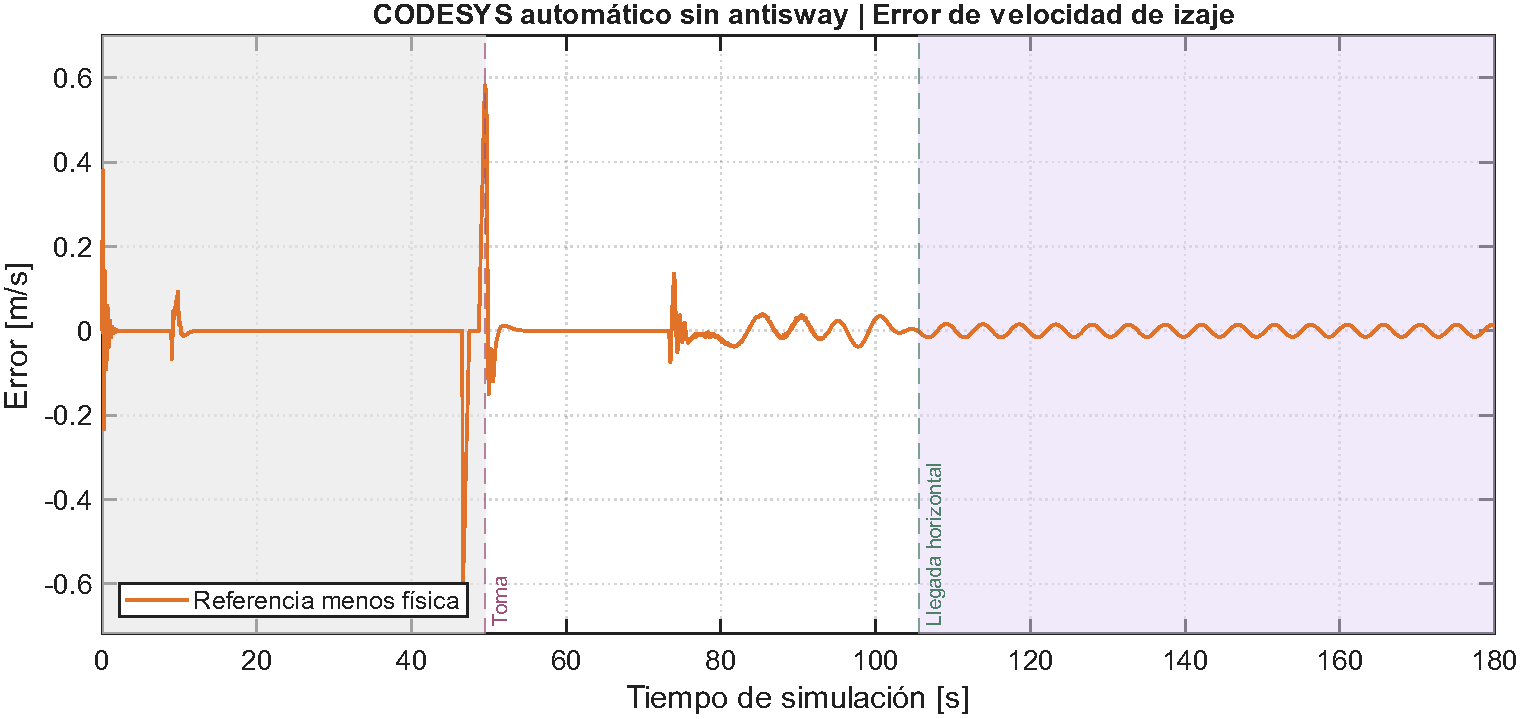
\includegraphics[width=0.98\textwidth]{graficas_individuales/automatico_sin_evy.pdf}
\caption{CODESYS automático sin antisway: Error de velocidad de izaje, calculado como referencia menos velocidad física.}\label{fig:individual_automatico_sin_evy}
\end{figure}

\begin{figure}[!htbp]
\centering
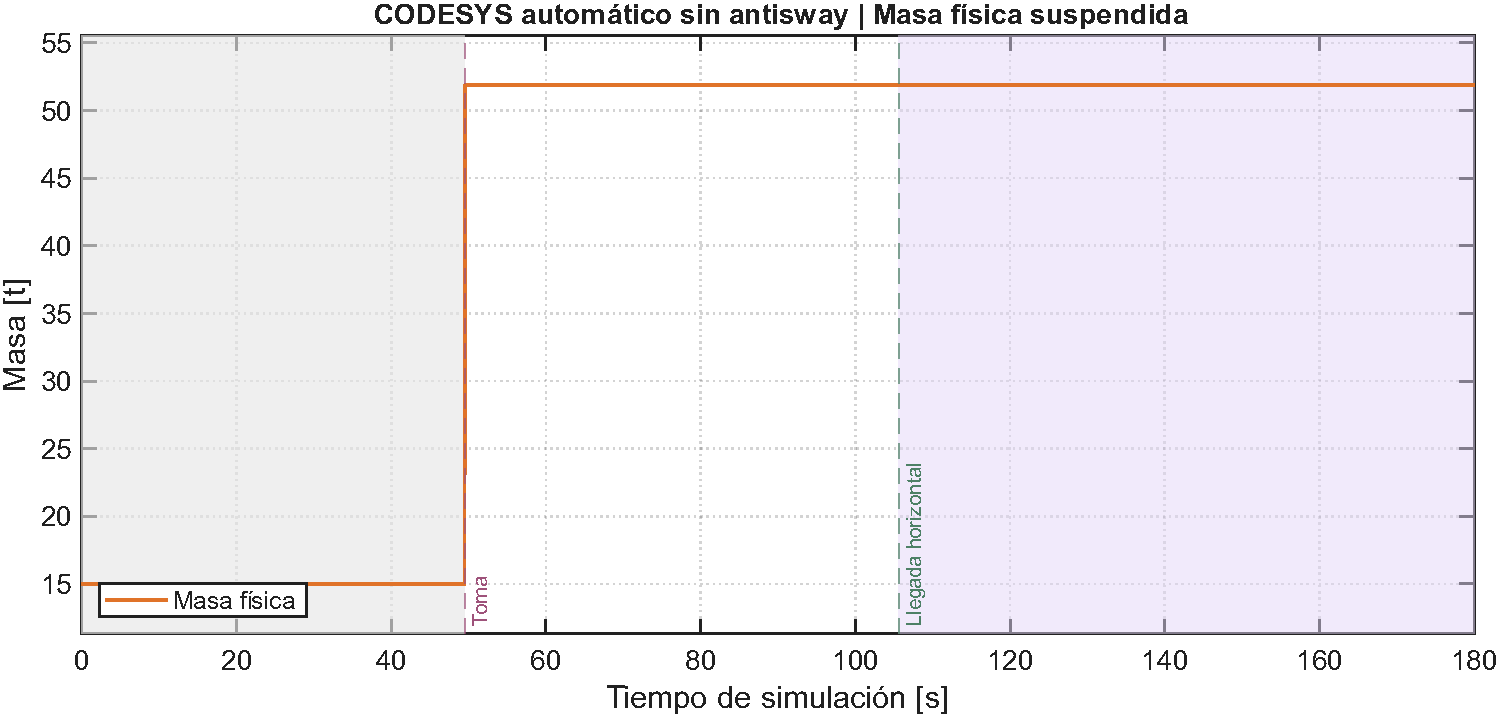
\includegraphics[width=0.98\textwidth]{graficas_individuales/automatico_sin_masa.pdf}
\caption{CODESYS automático sin antisway: Masa física suspendida: 51,863 t representa conjunto cargado y 15 t corresponde al spreader vacío.}\label{fig:individual_automatico_sin_masa}
\end{figure}

\begin{figure}[!htbp]
\centering
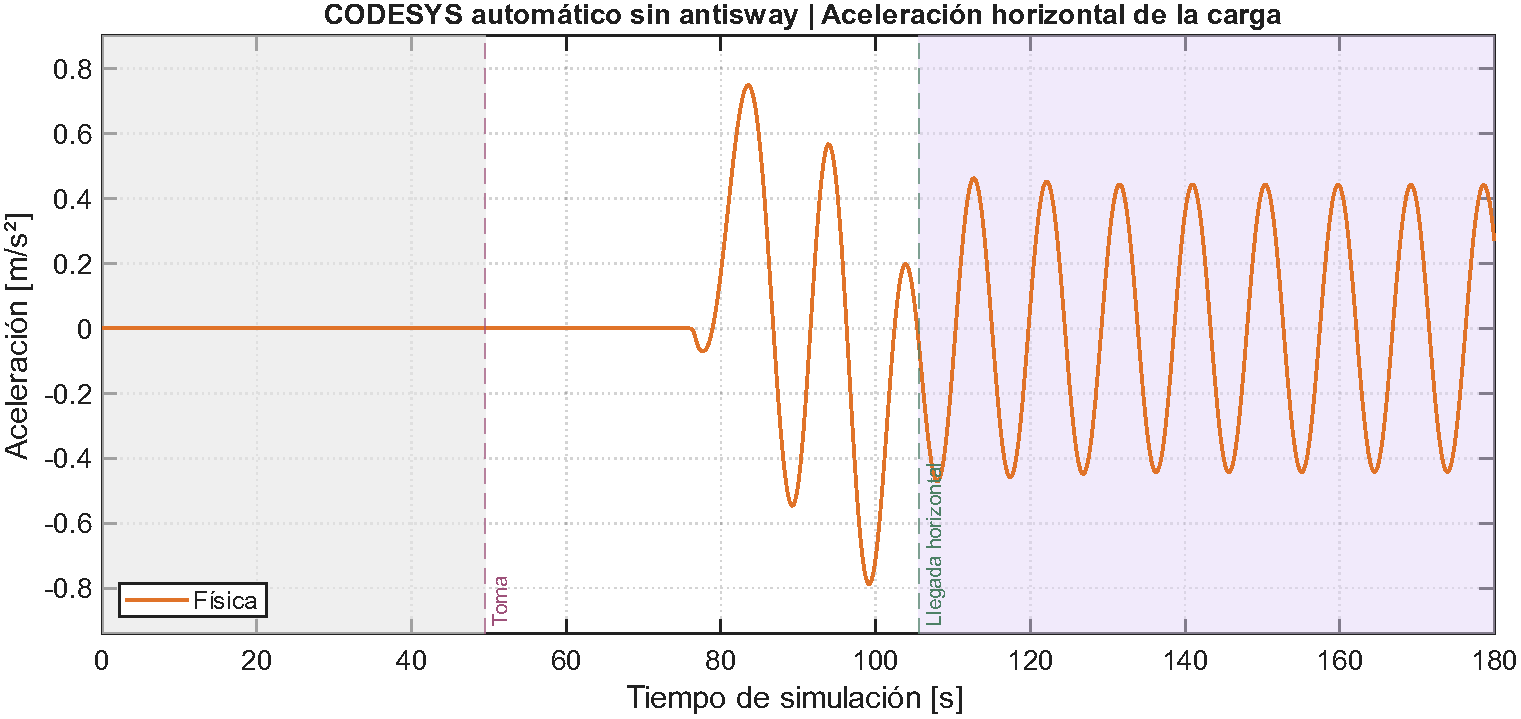
\includegraphics[width=0.98\textwidth]{graficas_individuales/automatico_sin_ax_carga.pdf}
\caption{CODESYS automático sin antisway: Aceleración horizontal física de la carga; se conservan las oscilaciones registradas.}\label{fig:individual_automatico_sin_ax_carga}
\end{figure}

\clearpage
\subsection{CODESYS automático con antisway: apoyo con descarga física bloqueada}
START ocurrió a $3.24~\mathrm{s}$, manual a $3.76~\mathrm{s}$ y cierre solicitado a $46.64~\mathrm{s}$. La masa cargada se confirmó a $49.52~\mathrm{s}$ y el despegue a $50.00~\mathrm{s}$. Automático se solicitó a $75.32~\mathrm{s}$ y fue observado por el operador a $75.40~\mathrm{s}$; el monitor de modo registra automático a $75.44~\mathrm{s}$. La llegada horizontal ocurrió a $105.76~\mathrm{s}$. Manual se solicitó a $133.20~\mathrm{s}$; el monitor registra el cambio a $133.24~\mathrm{s}$ y el operador lo confirmó a $133.56~\mathrm{s}$. Se distinguen estos tiempos porque la lectura y confirmación del operador añaden retardo respecto del monitor.

Con antisway se habilitó el avance del descenso y se alcanzó apoyo con solicitud de apertura a $169.24~\mathrm{s}$. Se permitió continuar más allá de tres minutos. Sin embargo, la planta mantuvo la carga: el diagnóstico a $272.52~\mathrm{s}$ mostró twistlocks abiertos y estado de carga vacío en el PLC, con contacto confirmado, mientras la masa física seguía siendo $51\,863~\mathrm{kg}$. Después de más de 100 s sin transferencia física en apoyo, se efectuó parada controlada de diagnóstico a $279.52~\mathrm{s}$.

\begin{figure}[!htbp]
\centering
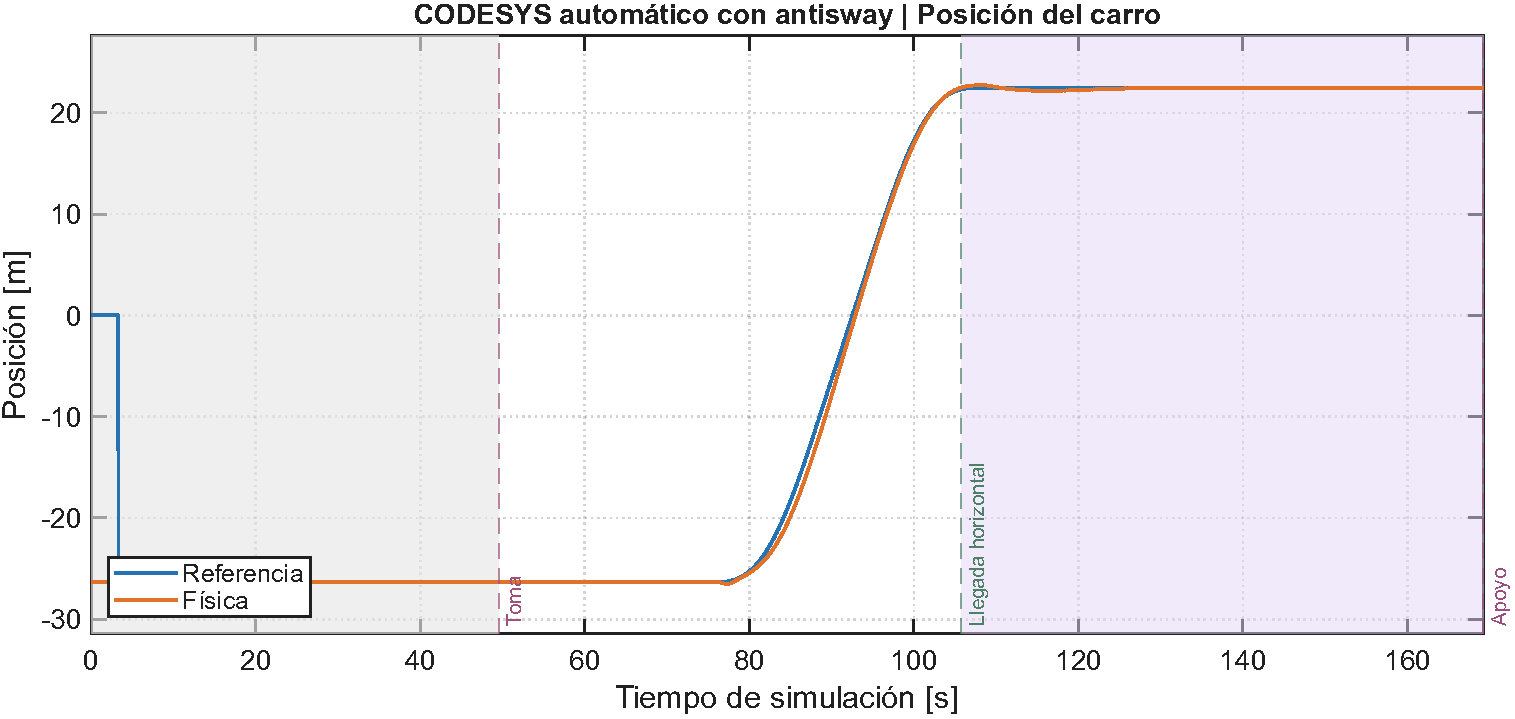
\includegraphics[width=0.98\textwidth]{graficas_individuales/automatico_con_x.pdf}
\caption{CODESYS automático con antisway: Posición del carro: referencia y evolución física.}\label{fig:individual_automatico_con_x}
\end{figure}

\begin{figure}[!htbp]
\centering
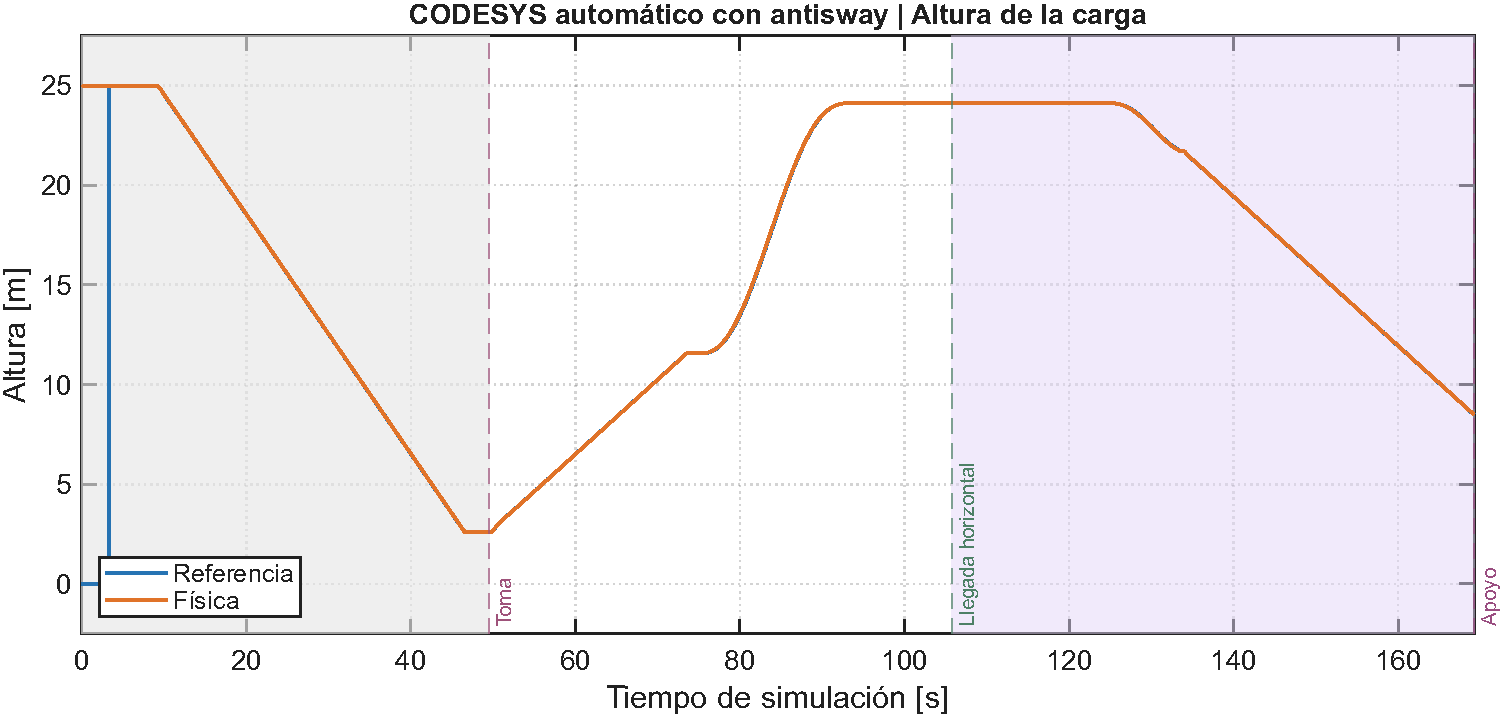
\includegraphics[width=0.98\textwidth]{graficas_individuales/automatico_con_y.pdf}
\caption{CODESYS automático con antisway: Altura de la carga: referencia y evolución física.}\label{fig:individual_automatico_con_y}
\end{figure}

\begin{figure}[!htbp]
\centering
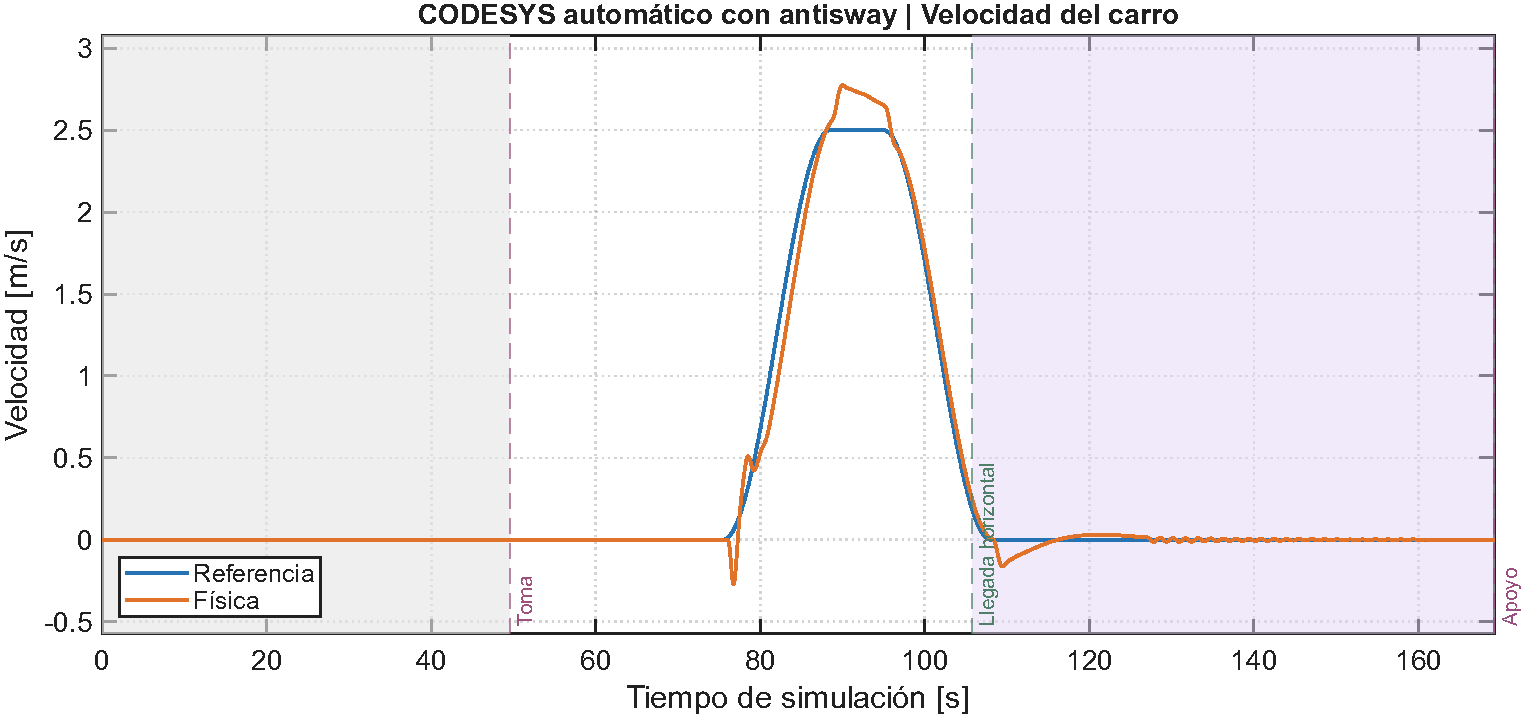
\includegraphics[width=0.98\textwidth]{graficas_individuales/automatico_con_vx.pdf}
\caption{CODESYS automático con antisway: Velocidad del carro: referencia y señal física.}\label{fig:individual_automatico_con_vx}
\end{figure}

\begin{figure}[!htbp]
\centering
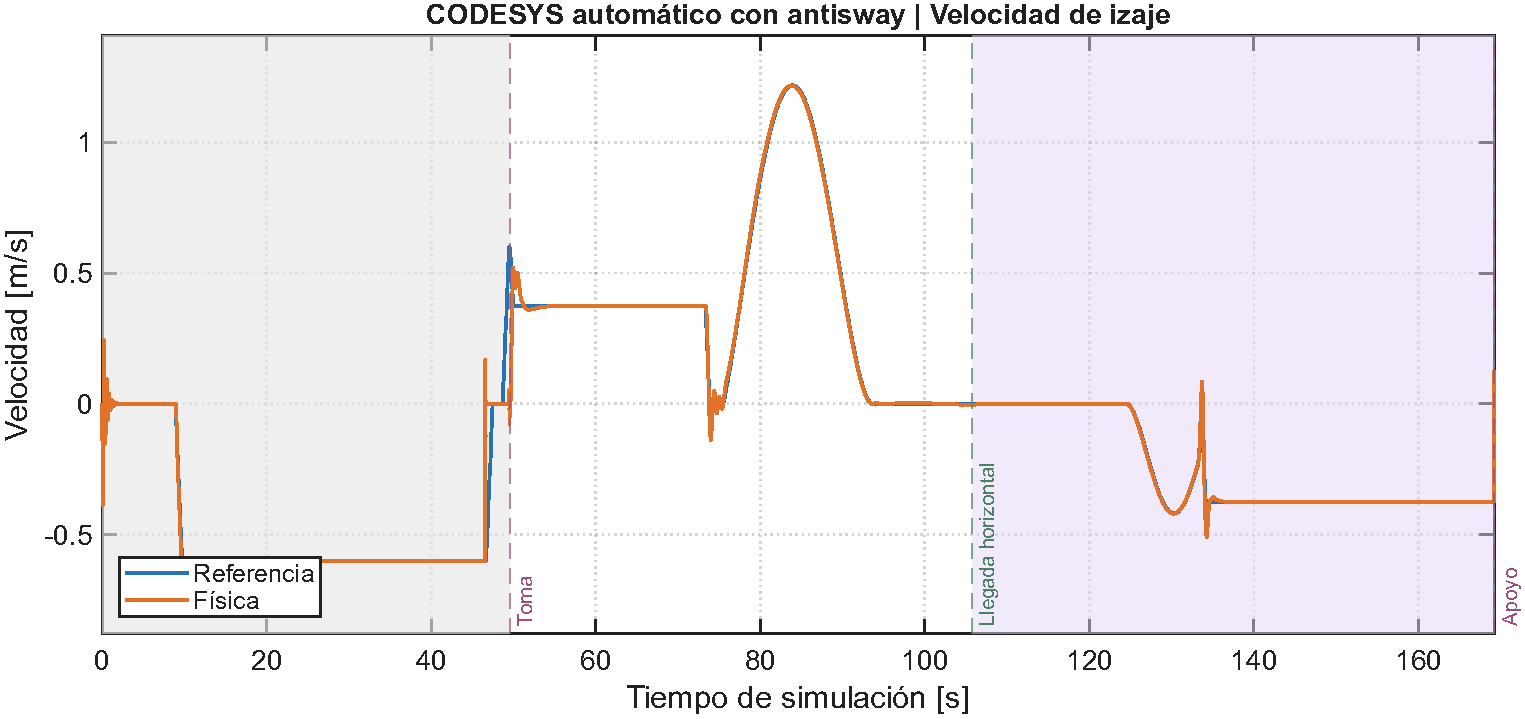
\includegraphics[width=0.98\textwidth]{graficas_individuales/automatico_con_vy.pdf}
\caption{CODESYS automático con antisway: Velocidad de izaje: referencia y señal física.}\label{fig:individual_automatico_con_vy}
\end{figure}

\begin{figure}[!htbp]
\centering
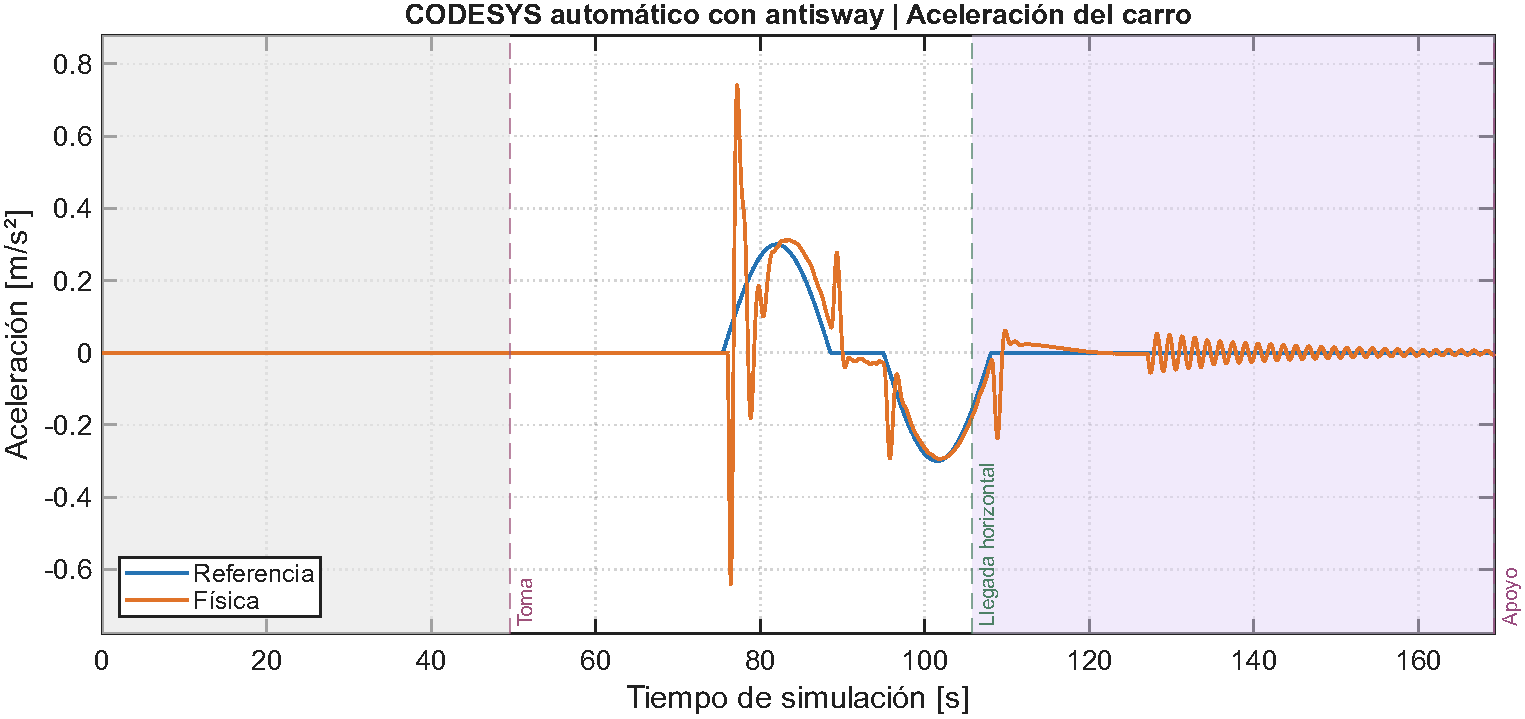
\includegraphics[width=0.98\textwidth]{graficas_individuales/automatico_con_ax.pdf}
\caption{CODESYS automático con antisway: Aceleración del carro: referencia y señal física.}\label{fig:individual_automatico_con_ax}
\end{figure}

\begin{figure}[!htbp]
\centering
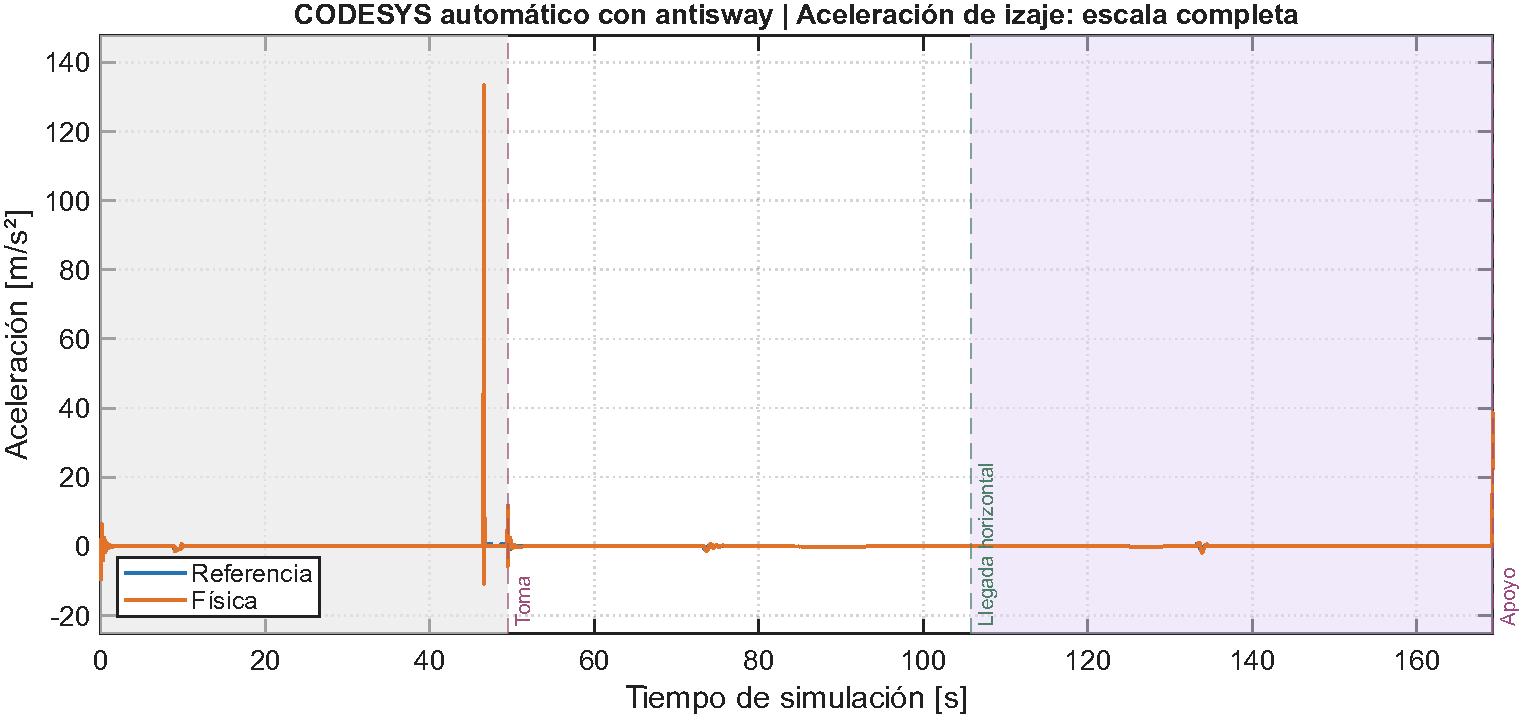
\includegraphics[width=0.98\textwidth]{graficas_individuales/automatico_con_ay.pdf}
\caption{CODESYS automático con antisway: Aceleración de izaje en escala completa; se conservan los picos de contacto y arranque.}\label{fig:individual_automatico_con_ay}
\end{figure}

\begin{figure}[!htbp]
\centering
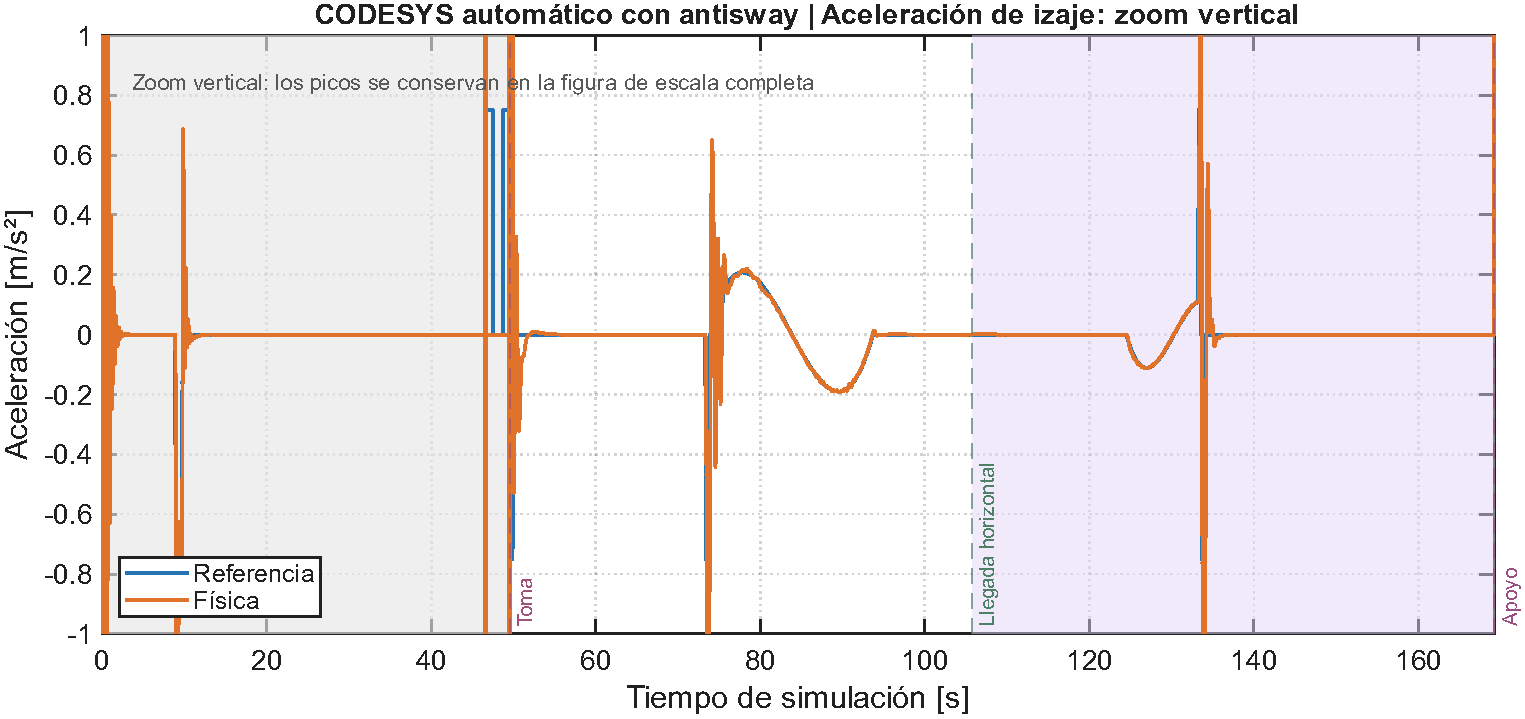
\includegraphics[width=0.98\textwidth]{graficas_individuales/automatico_con_ay_zoom.pdf}
\caption{CODESYS automático con antisway: Aceleración de izaje con zoom vertical entre $-1$ y $+1~\mathrm{m/s^2}$ para observar su evolución temporal. Los picos que exceden este intervalo permanecen visibles en la figura de escala completa; no se filtraron las señales.}\label{fig:individual_automatico_con_ay_zoom}
\end{figure}

\begin{figure}[!htbp]
\centering
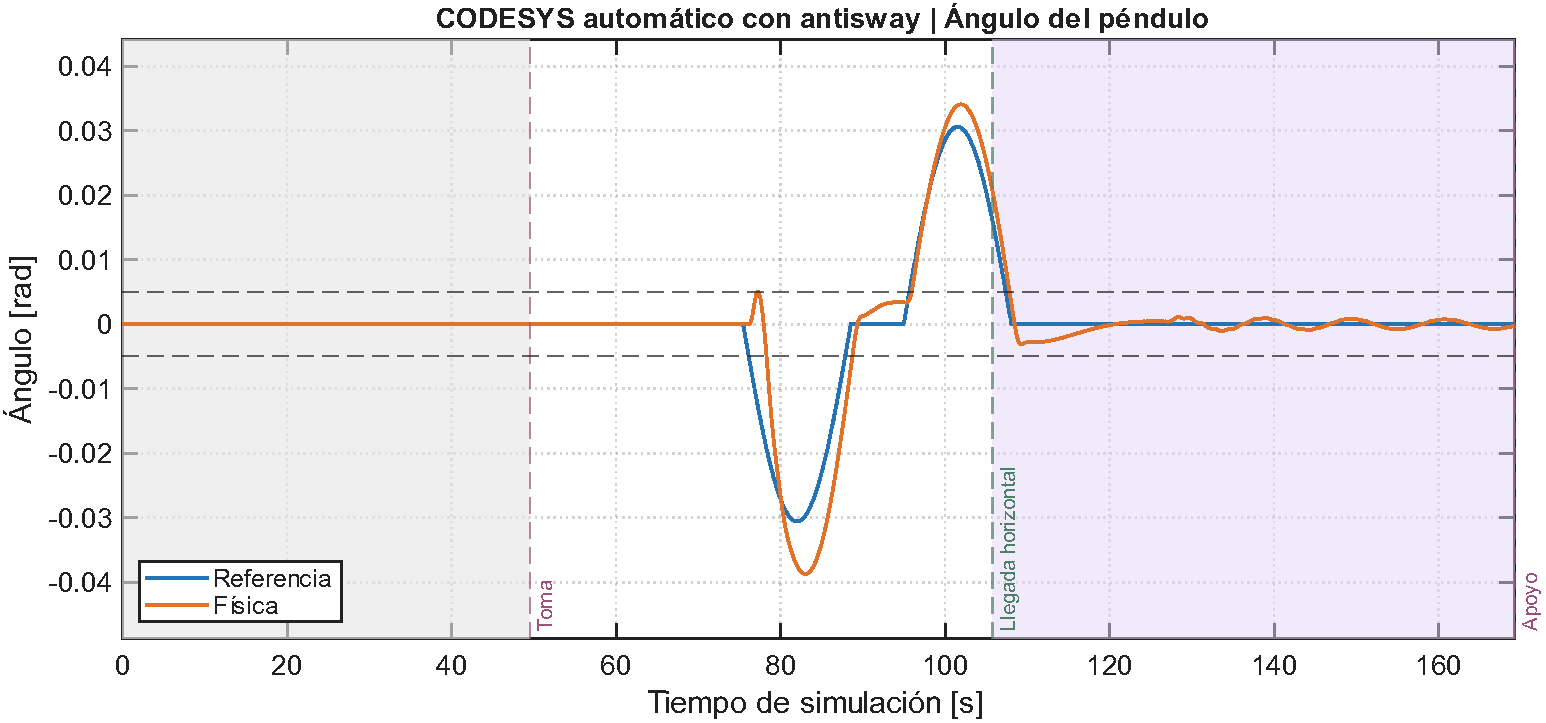
\includegraphics[width=0.98\textwidth]{graficas_individuales/automatico_con_theta.pdf}
\caption{CODESYS automático con antisway: Ángulo físico y de referencia del péndulo. Las líneas horizontales señalan los umbrales angulares del descenso.}\label{fig:individual_automatico_con_theta}
\end{figure}

\begin{figure}[!htbp]
\centering
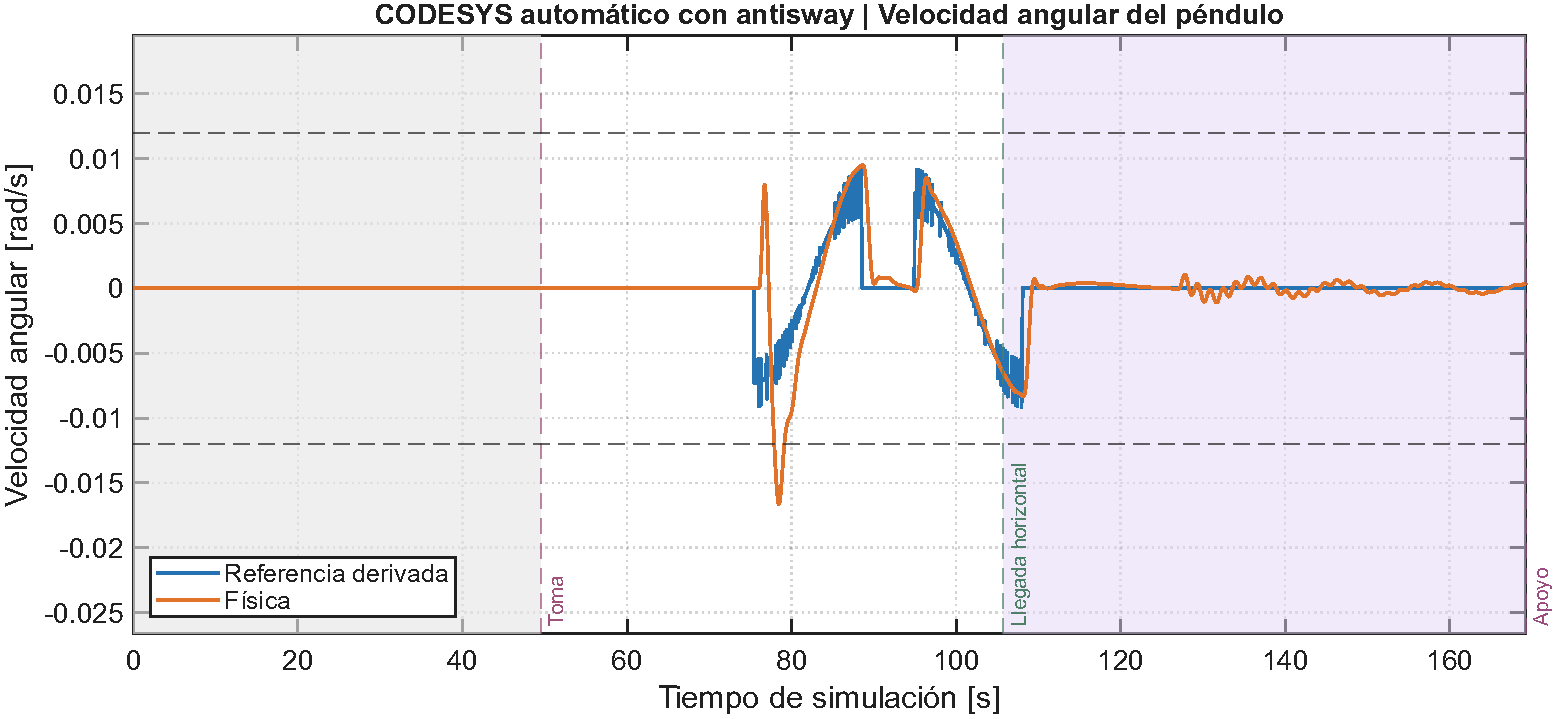
\includegraphics[width=0.98\textwidth]{graficas_individuales/automatico_con_omega.pdf}
\caption{CODESYS automático con antisway: Velocidad angular física y referencia derivada numéricamente; se distinguen ambas fuentes. Las líneas horizontales indican los umbrales del descenso.}\label{fig:individual_automatico_con_omega}
\end{figure}

\begin{figure}[!htbp]
\centering
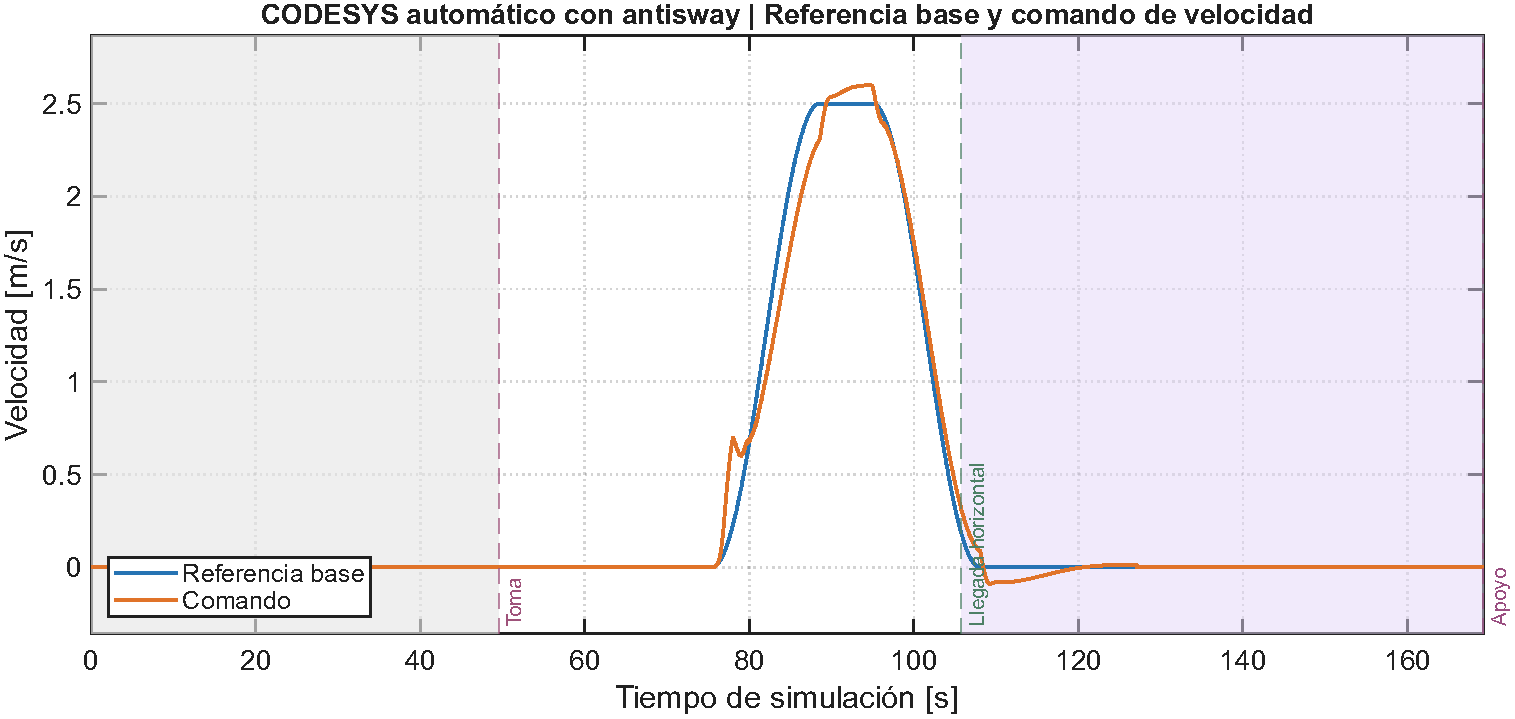
\includegraphics[width=0.98\textwidth]{graficas_individuales/automatico_con_vcmd.pdf}
\caption{CODESYS automático con antisway: Referencia base y comando de velocidad; su diferencia corresponde a la contribución antisway efectiva en el sumador.}\label{fig:individual_automatico_con_vcmd}
\end{figure}

\begin{figure}[!htbp]
\centering
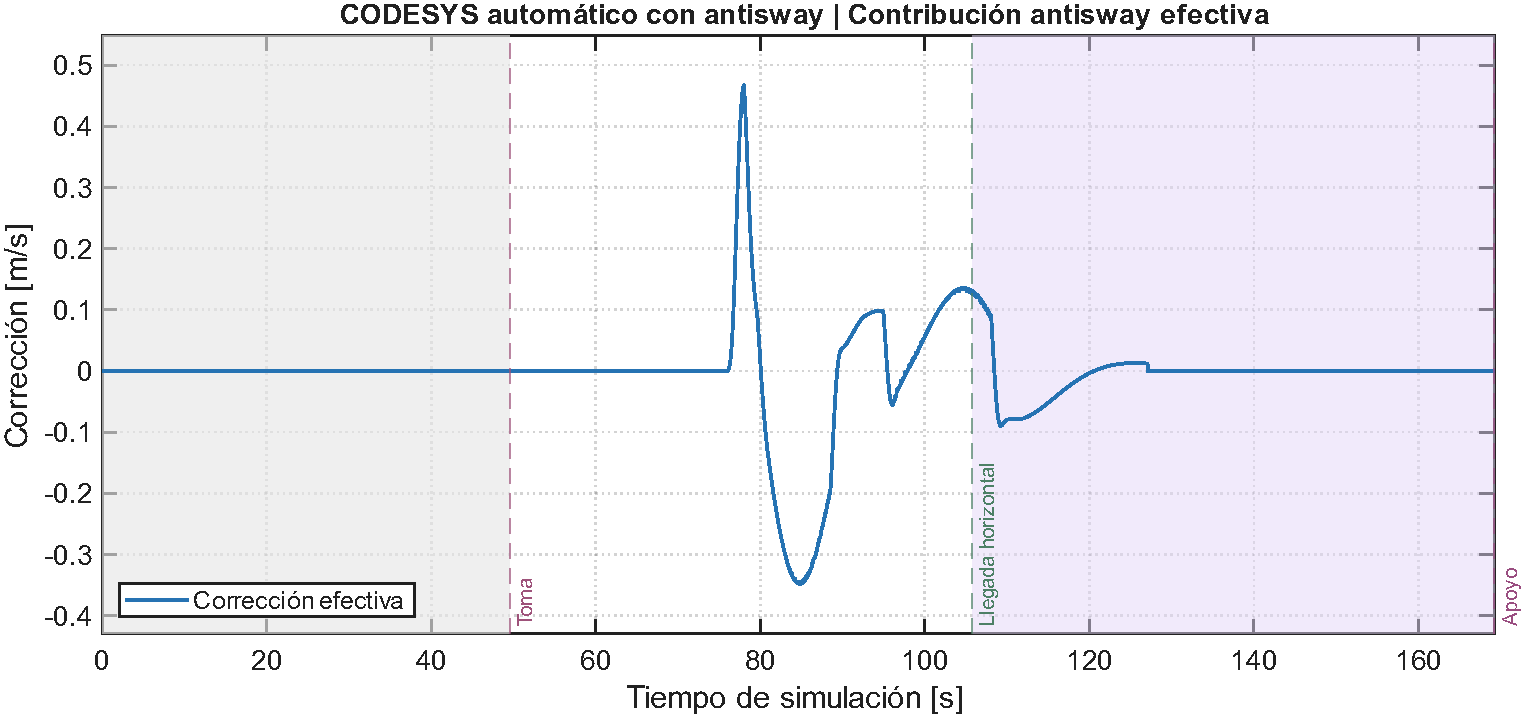
\includegraphics[width=0.98\textwidth]{graficas_individuales/automatico_con_sw.pdf}
\caption{CODESYS automático con antisway: Contribución antisway efectivamente sumada al comando de velocidad.}\label{fig:individual_automatico_con_sw}
\end{figure}

La contribución antisway máxima nativa fue $0.46702~\mathrm{m/s}$, verificada sobre $279\,521$ muestras. El carro terminó en $22.43043~\mathrm{m}$ y la carga en $8.48983~\mathrm{m}$; el error horizontal fue $0.02957~\mathrm{m}$. El origen disminuyó $2.59~\mathrm{m}$, pero el destino no aumentó. La proximidad al destino y el estado vacío del PLC no reemplazan esas comprobaciones físicas.

La lógica física de descarga exige simultáneamente apertura, contacto, velocidad vertical pequeña y desactivación de la histéresis de tensión. En el diagnóstico, la tensión fue aproximadamente $99.54~\mathrm{kN}$, superior al umbral de desactivación de $15.009~\mathrm{kN}$. La histéresis permaneció activa y bloqueó la transferencia del contenedor. En la espera final, la consigna de torque de izaje continúa descendiendo mientras el torque de motor alcanza una meseta próxima a -20 kN m; la diferencia entre consigna y actuación muestra que la orden adicional no se traduce en el mismo incremento de torque físico. Los errores de seguimiento crecen durante la espera final porque la referencia del PLC deja de corresponder al estado cargado que persiste en la planta; no representan una nueva maniobra de entrega completada. Esta observación complementa el diagnóstico de tensión y no constituye por sí sola identificación de la causa raíz. Ésta es la condición inmediata observada; los datos no prueban que la causa raíz pertenezca al generador de código. Debe revisarse la coordinación de apoyo, referencia de izaje y confirmación de descarga antes de atribuir el resultado a PLC Coder. No se forzaron masa, estado de carga ni umbrales para declarar entrega.

\begin{figure}[!htbp]
\centering
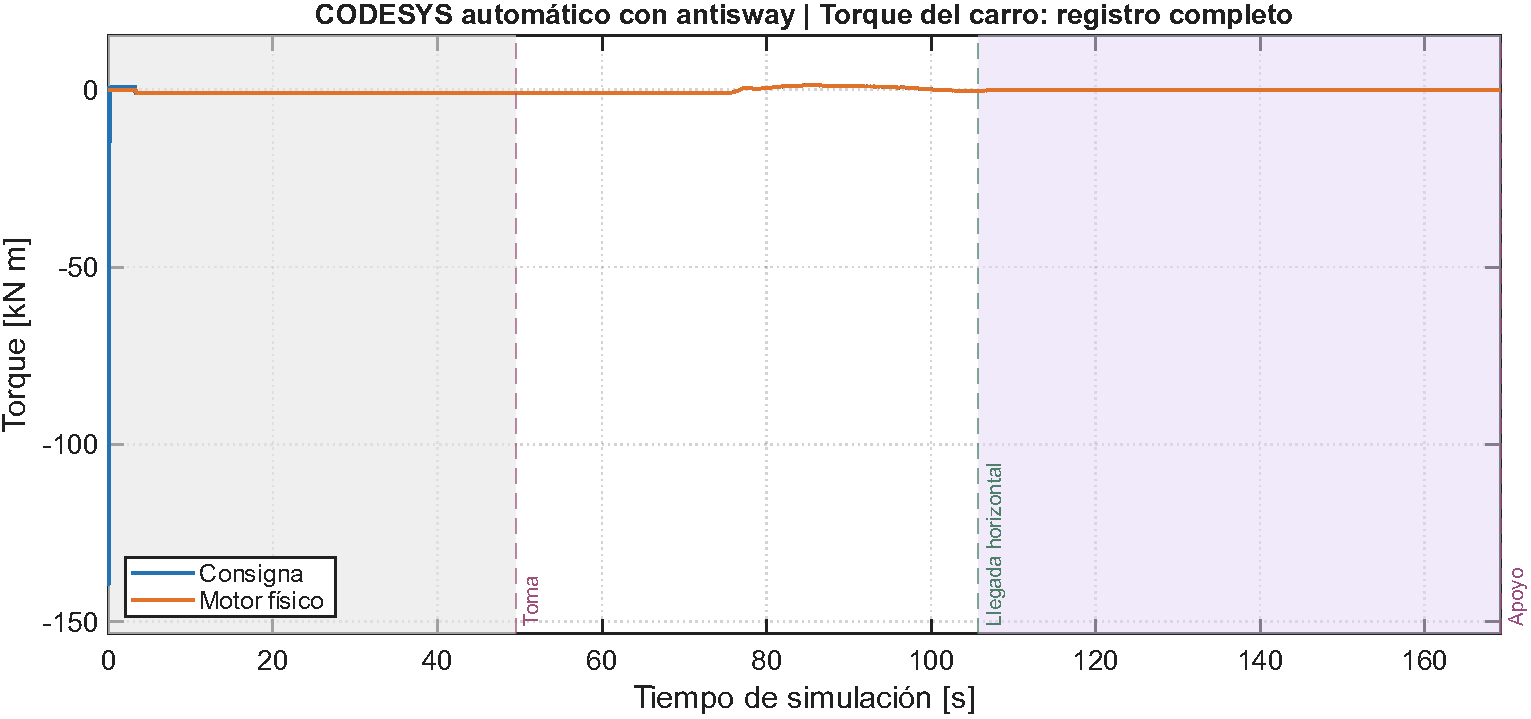
\includegraphics[width=0.98\textwidth]{graficas_individuales/automatico_con_tx.pdf}
\caption{CODESYS automático con antisway: Consigna y torque físico del motor del carro en el intervalo representado, incluido el arranque.}\label{fig:individual_automatico_con_tx}
\end{figure}

\begin{figure}[!htbp]
\centering
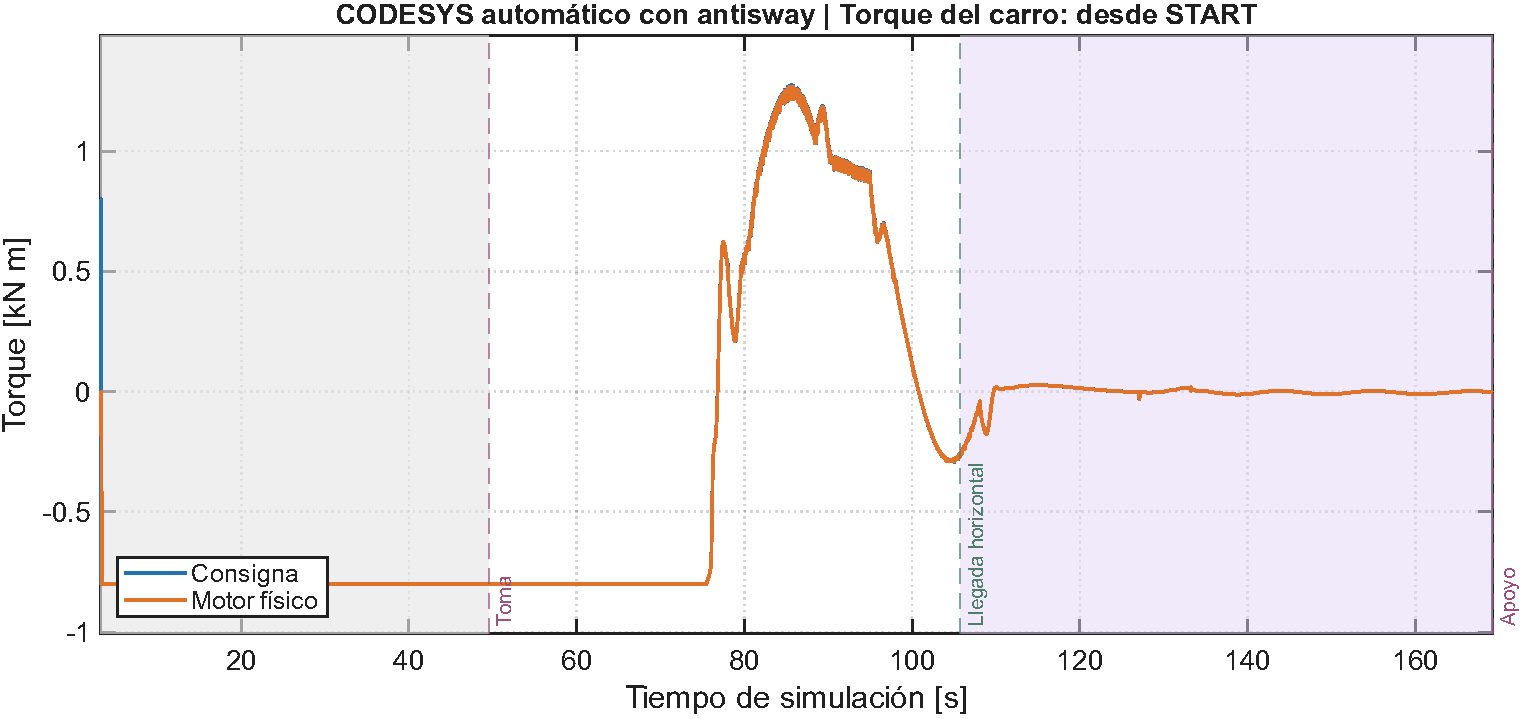
\includegraphics[width=0.98\textwidth]{graficas_individuales/automatico_con_tx_zoom.pdf}
\caption{CODESYS automático con antisway: Consigna y torque físico del motor del carro desde START; la escala completa del arranque se conserva en una figura independiente.}\label{fig:individual_automatico_con_tx_zoom}
\end{figure}

\begin{figure}[!htbp]
\centering
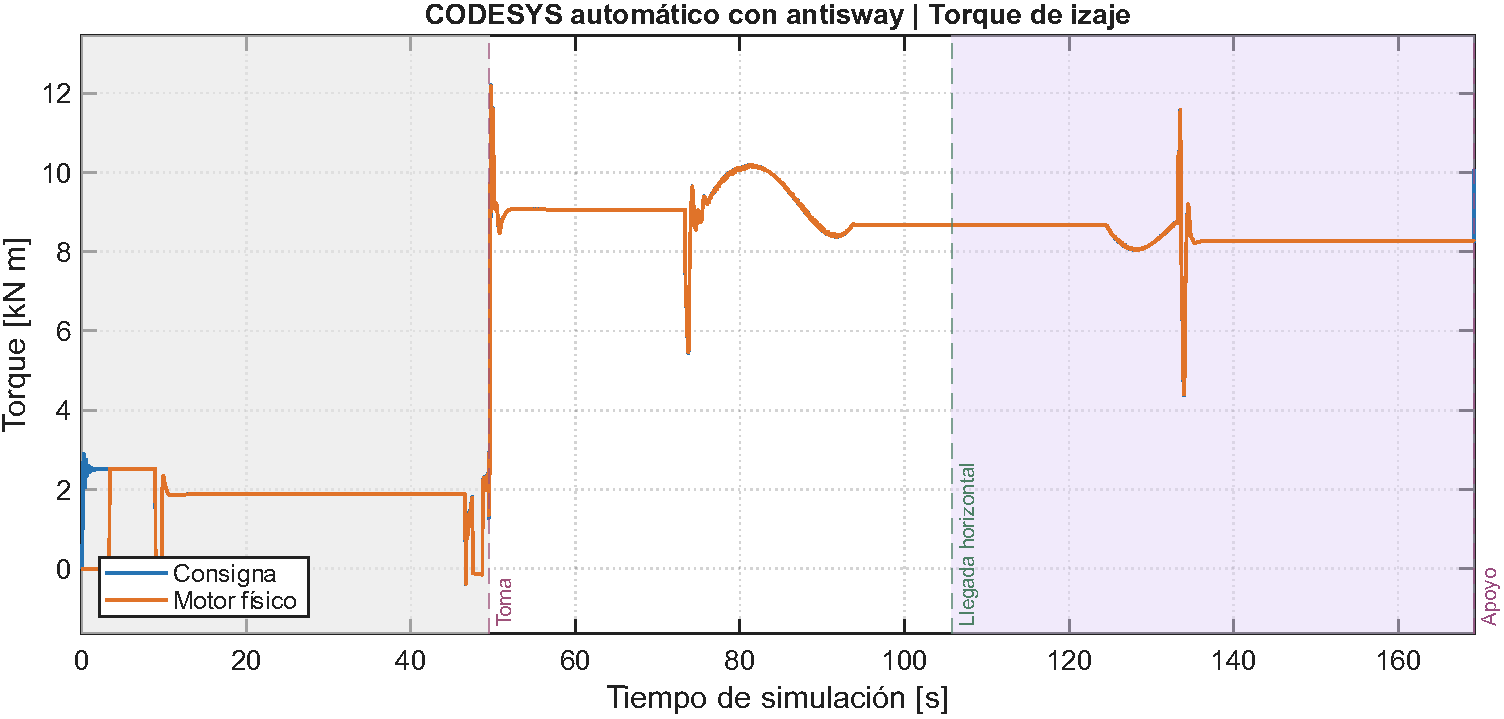
\includegraphics[width=0.98\textwidth]{graficas_individuales/automatico_con_ty.pdf}
\caption{CODESYS automático con antisway: Consigna del controlador y torque físico del motor de izaje.}\label{fig:individual_automatico_con_ty}
\end{figure}

\begin{figure}[!htbp]
\centering
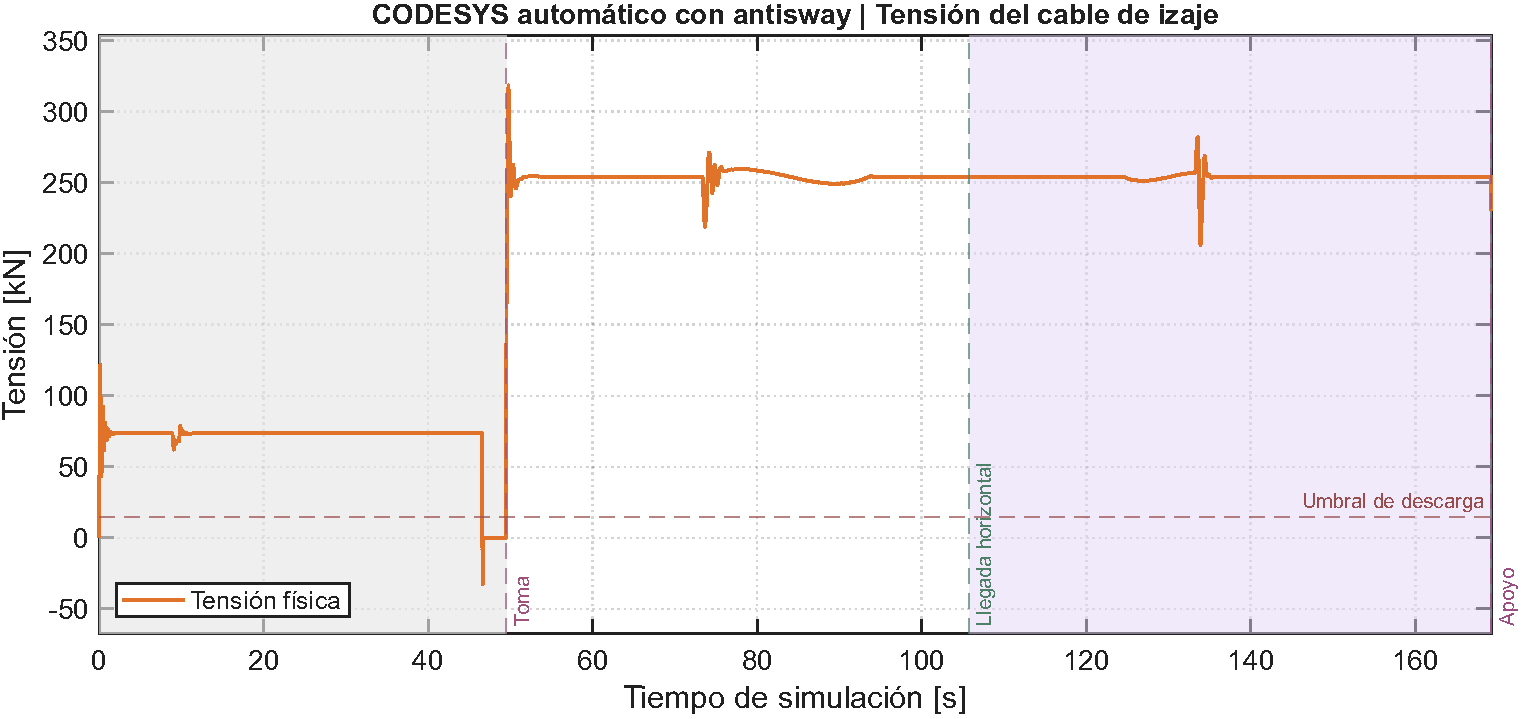
\includegraphics[width=0.98\textwidth]{graficas_individuales/automatico_con_tension.pdf}
\caption{CODESYS automático con antisway: Tensión física del cable de izaje. Se conserva el umbral de descarga como referencia; el diagnóstico posterior al intento de entrega se describe en el texto y queda fuera de esta ventana gráfica.}\label{fig:individual_automatico_con_tension}
\end{figure}

\begin{figure}[!htbp]
\centering
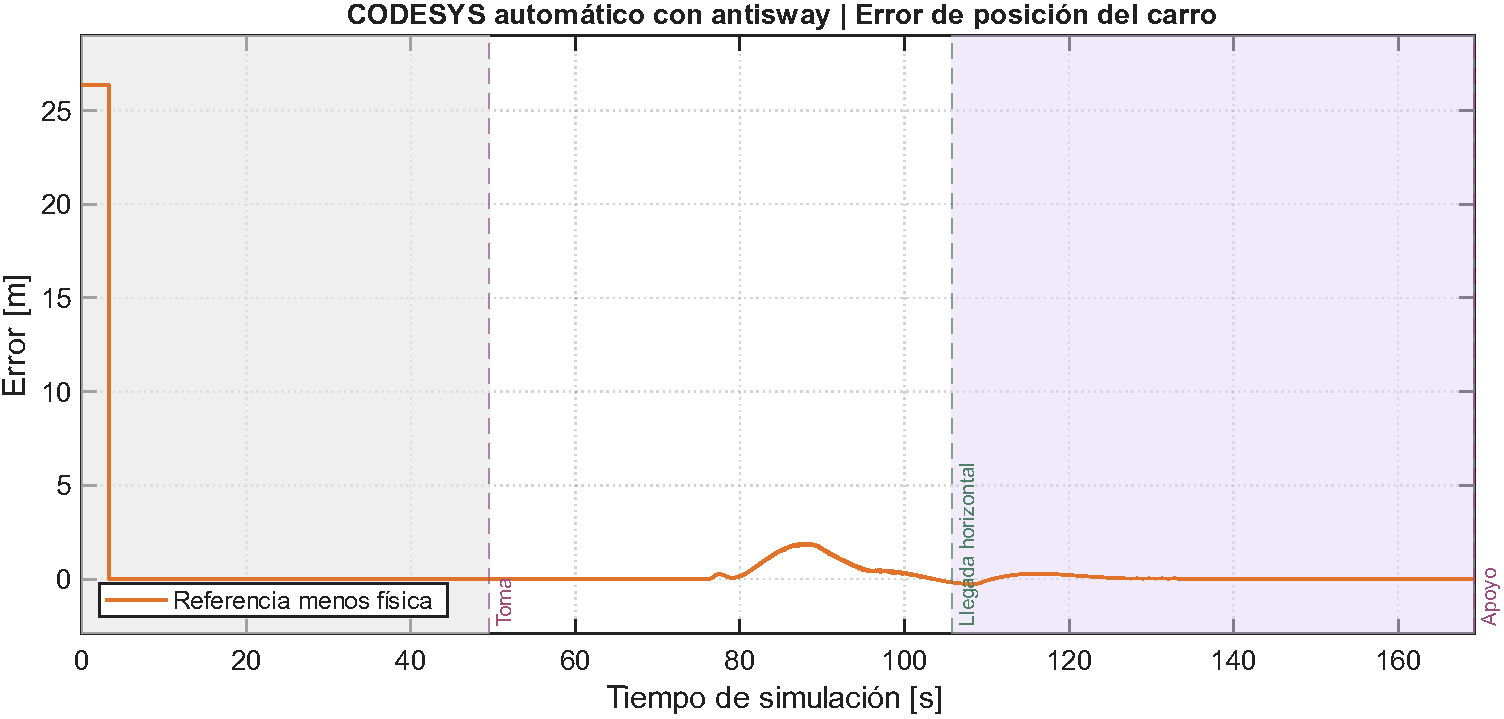
\includegraphics[width=0.98\textwidth]{graficas_individuales/automatico_con_ex.pdf}
\caption{CODESYS automático con antisway: Error horizontal, calculado como referencia menos posición física.}\label{fig:individual_automatico_con_ex}
\end{figure}

\begin{figure}[!htbp]
\centering
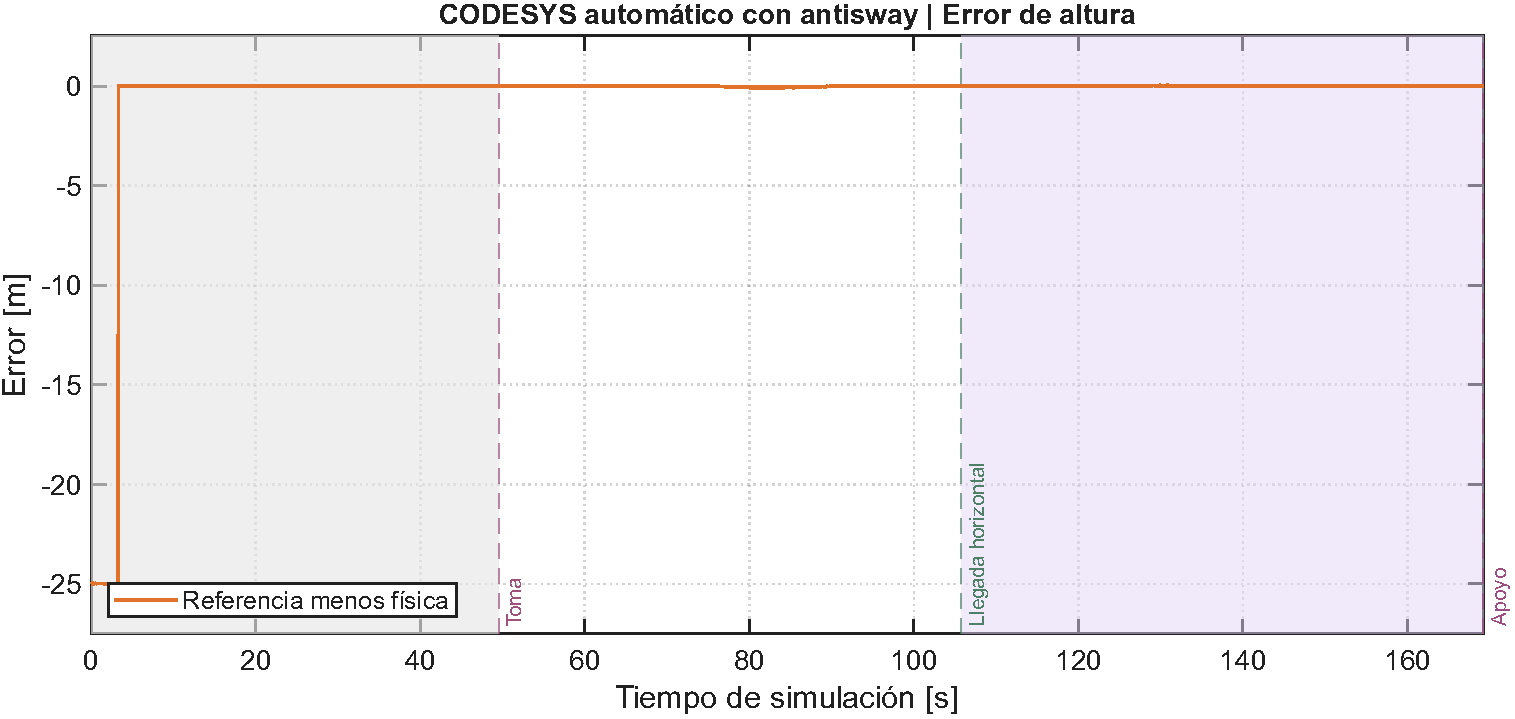
\includegraphics[width=0.98\textwidth]{graficas_individuales/automatico_con_ey.pdf}
\caption{CODESYS automático con antisway: Error de altura, calculado como referencia menos altura física.}\label{fig:individual_automatico_con_ey}
\end{figure}

\begin{figure}[!htbp]
\centering
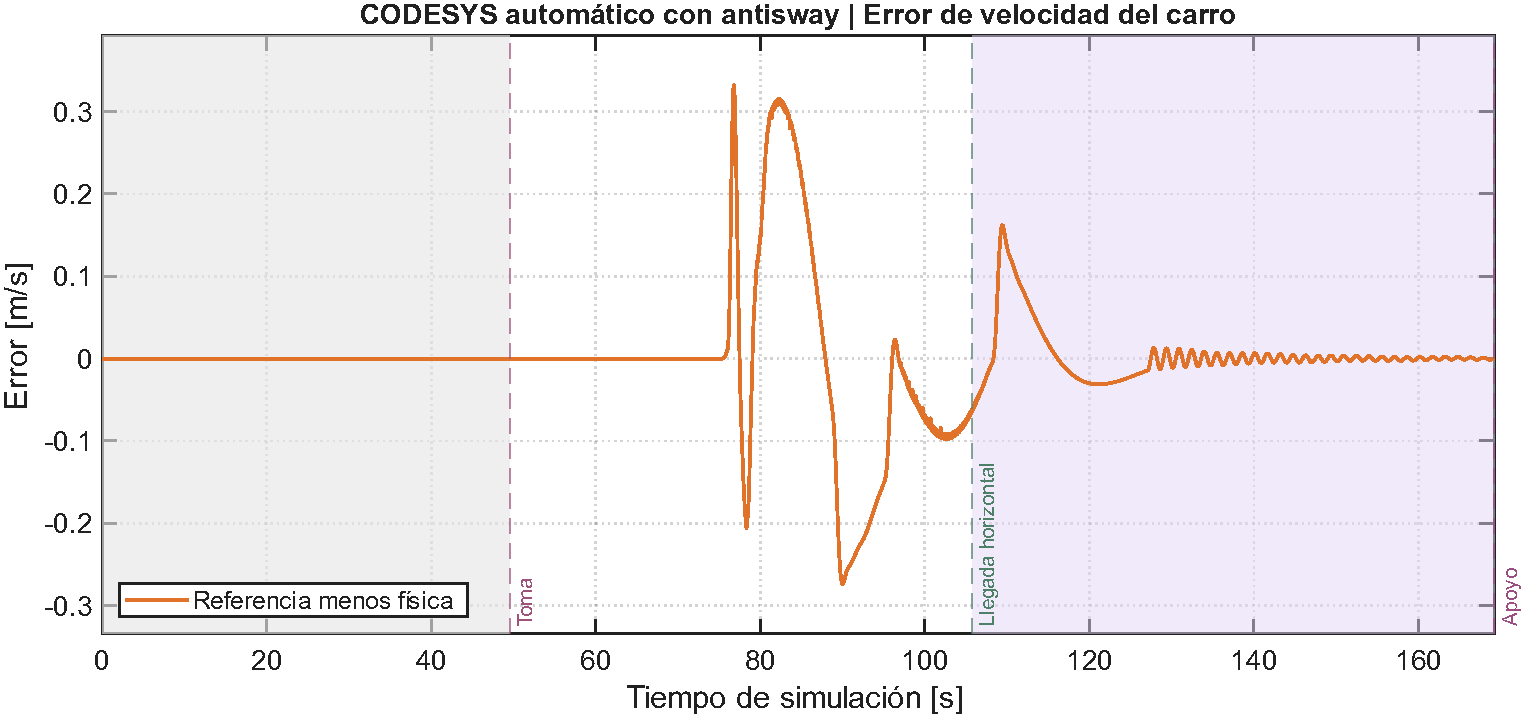
\includegraphics[width=0.98\textwidth]{graficas_individuales/automatico_con_evx.pdf}
\caption{CODESYS automático con antisway: Error de velocidad del carro, calculado como referencia menos velocidad física.}\label{fig:individual_automatico_con_evx}
\end{figure}

\begin{figure}[!htbp]
\centering
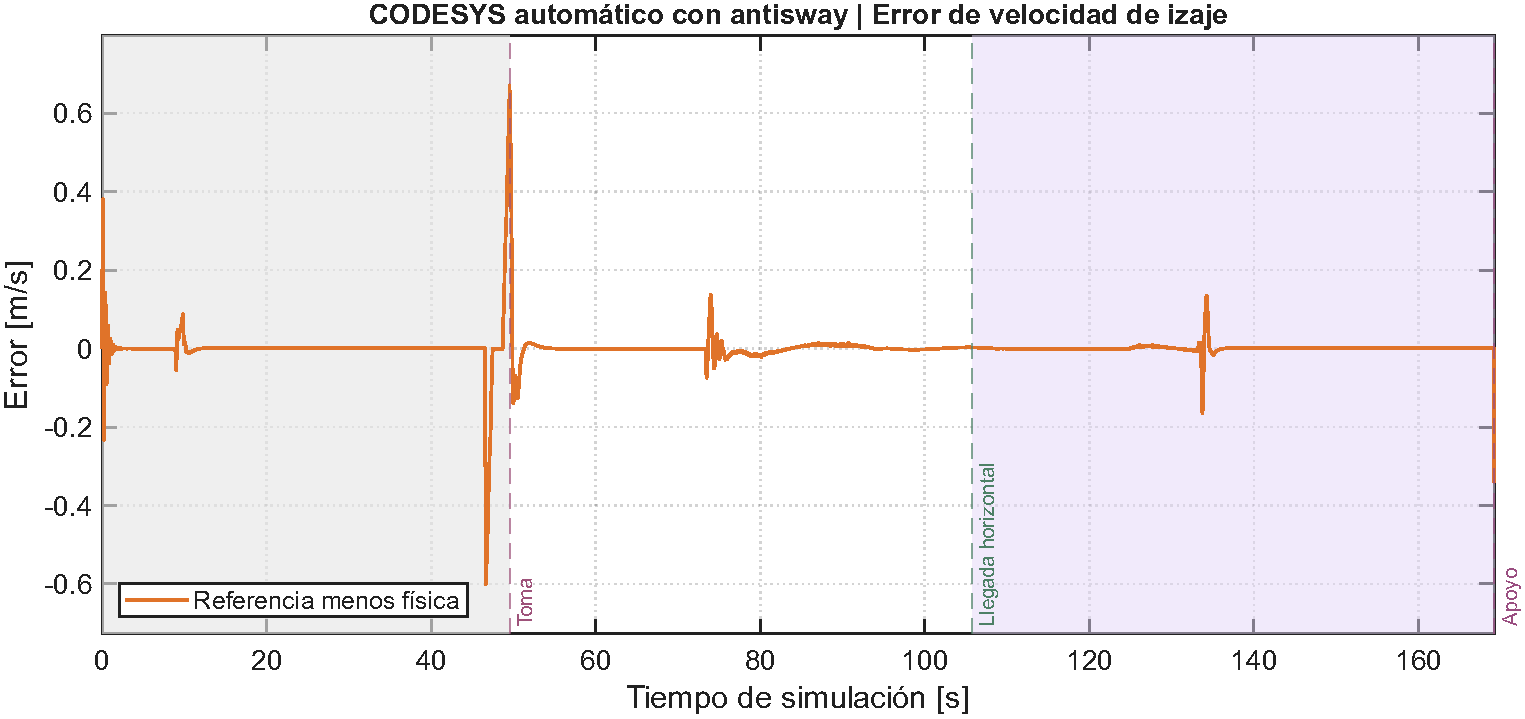
\includegraphics[width=0.98\textwidth]{graficas_individuales/automatico_con_evy.pdf}
\caption{CODESYS automático con antisway: Error de velocidad de izaje, calculado como referencia menos velocidad física.}\label{fig:individual_automatico_con_evy}
\end{figure}

\begin{figure}[!htbp]
\centering
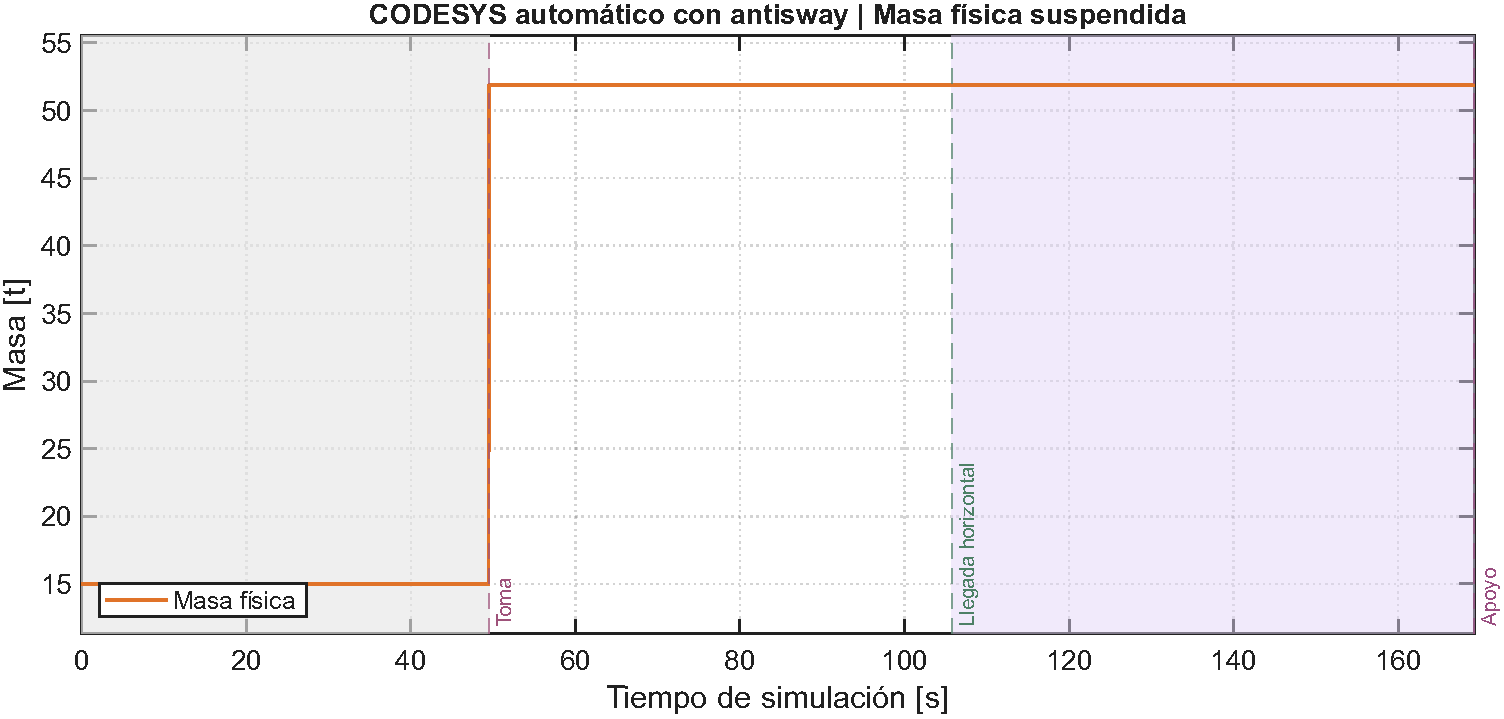
\includegraphics[width=0.98\textwidth]{graficas_individuales/automatico_con_masa.pdf}
\caption{CODESYS automático con antisway: Masa física suspendida: 51,863 t representa conjunto cargado y 15 t corresponde al spreader vacío.}\label{fig:individual_automatico_con_masa}
\end{figure}

\begin{figure}[!htbp]
\centering
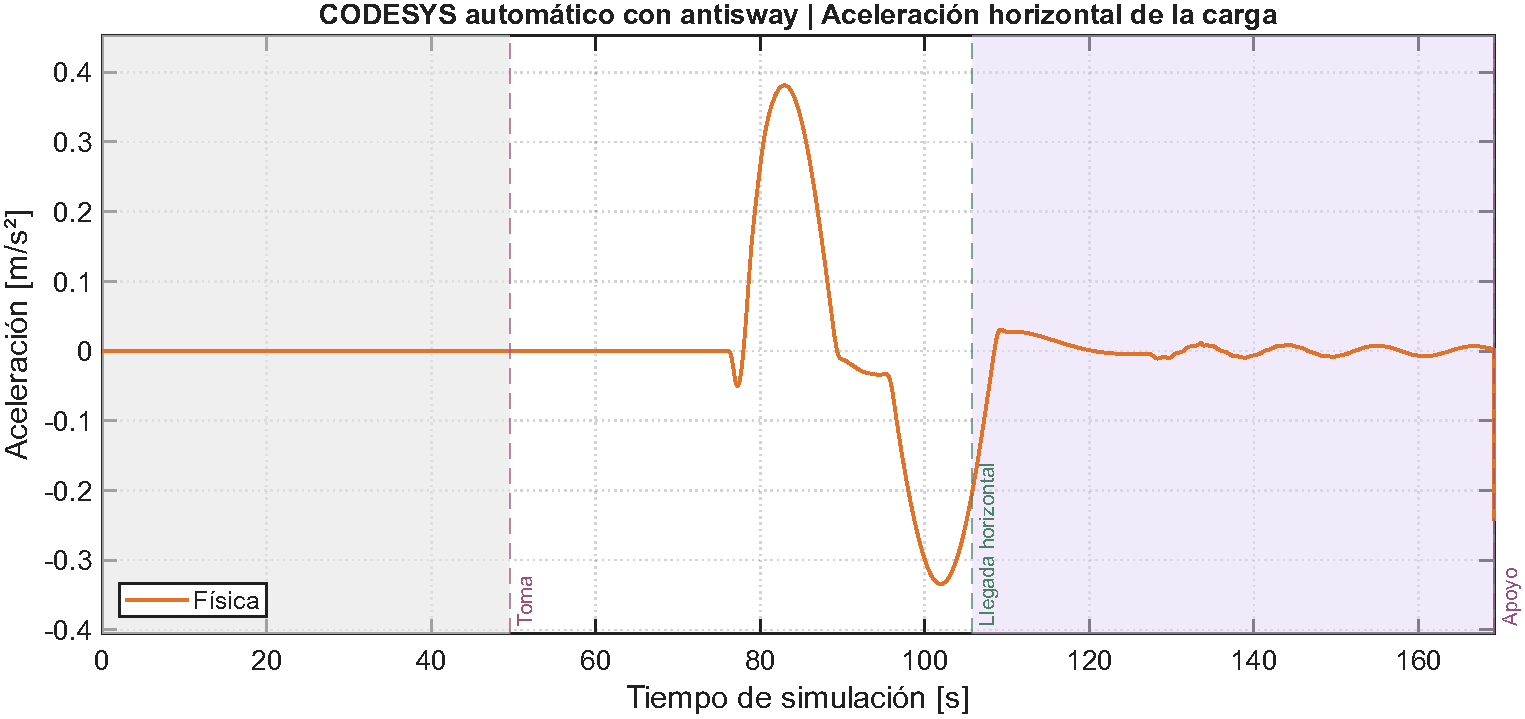
\includegraphics[width=0.98\textwidth]{graficas_individuales/automatico_con_ax_carga.pdf}
\caption{CODESYS automático con antisway: Aceleración horizontal física de la carga; se conservan las oscilaciones registradas.}\label{fig:individual_automatico_con_ax_carga}
\end{figure}

\clearpage
\section{Comparación experimental entre CODESYS manual y automático}
\label{sec:comparacion_ensayos_codesys}
\subsection{Resultados físicos de las cuatro pruebas}
La \cref{tab:resultado_cuatro_codesys} resume las corridas actuales. Sólo CODESYS manual con antisway completó la entrega. Las dos pruebas sin antisway terminaron con carga retenida en la zona de cruce; CODESYS automático con antisway alcanzó apoyo pero conservó la carga física. Las duraciones de parada por límite o diagnóstico no son tiempos de ciclo productivo y no permiten ordenar las implementaciones por rendimiento.

\begin{table}[!htbp]\centering\small
\caption{Estado final y resultado de las cuatro pruebas actualizadas.}\label{tab:resultado_cuatro_codesys}
\begin{tabular}{L{.28\textwidth}C{.10\textwidth}C{.15\textwidth}L{.35\textwidth}}\toprule
Prueba & Fin [s] & Masa final [kg] & Resultado\\\midrule
CODESYS manual sin antisway & 187.20 & 51\,863 & Sin entrega; parada solicitada. Registro nativo parcial.\\
CODESYS manual con antisway & 169.20 & 15\,000 & Entrega física confirmada y parada.\\
CODESYS automático sin antisway & 180.00 & 51\,863 & Sin entrega; límite programado.\\
CODESYS automático con antisway & 279.52 & 51\,863 & Apoyo alcanzado; descarga física bloqueada; parada diagnóstica.\\\bottomrule
\end{tabular}\end{table}

Las trayectorias absolutas de la \cref{fig:individual_comparacion_x,fig:individual_comparacion_y,fig:individual_comparacion_theta,fig:individual_comparacion_masa} conservan cada duración. Su superposición ilustra el resultado y los distintos finales; no calcula RMS de un ciclo completo frente a otro incompleto. Las comparaciones cuantitativas de etapas deben limitarse a fases completadas por ambas variantes, como la toma y el despegue. La espera prolongada y el apoyo bloqueado se interpretan como diagnóstico, sin incorporarlos como mejora aparente del RMS ni como entregas completadas.

\begin{figure}[!htbp]
\centering
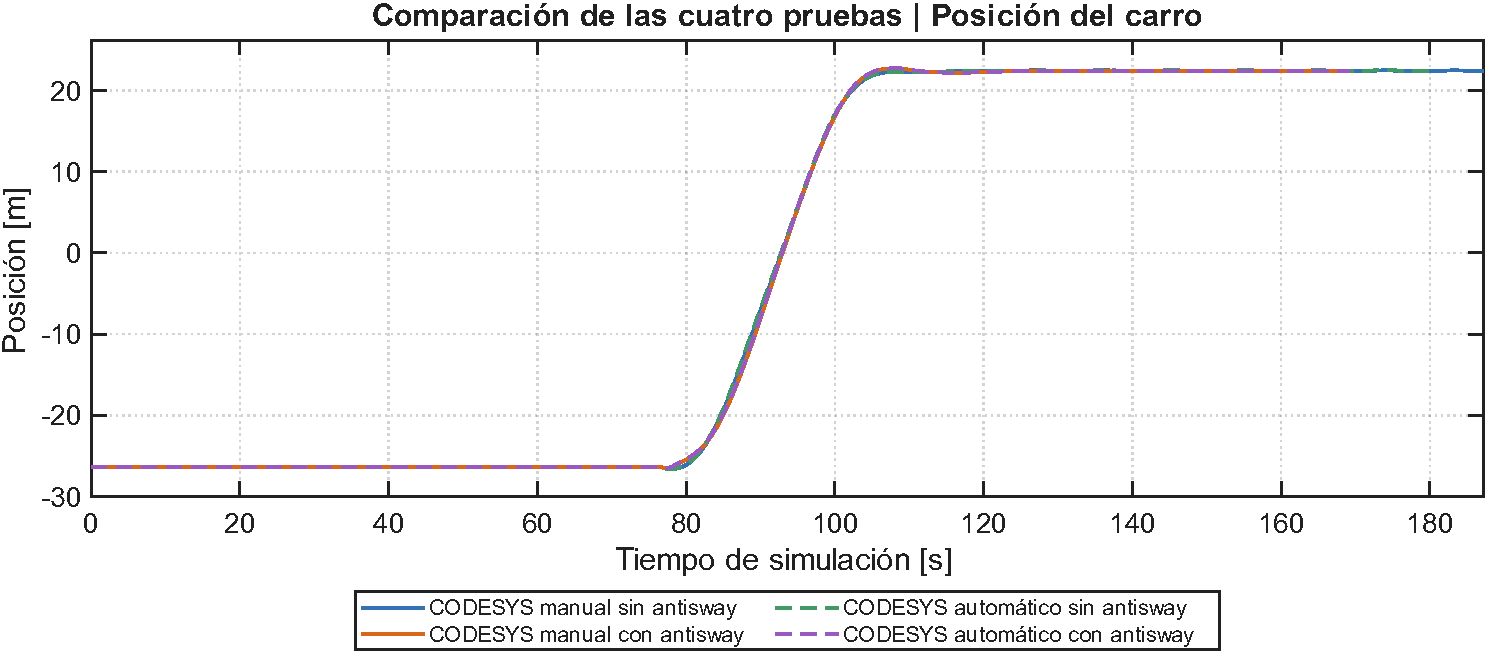
\includegraphics[width=0.98\textwidth]{graficas_individuales/comparacion_x.pdf}
\caption{Comparación de las cuatro pruebas: posición del carro. Las curvas con antisway terminan en el apoyo o intento de entrega: 168,92 s para CODESYS manual y 169,24 s para CODESYS automático. Las variantes sin antisway conservan su duración y cobertura disponibles.}\label{fig:individual_comparacion_x}
\end{figure}

\begin{figure}[!htbp]
\centering
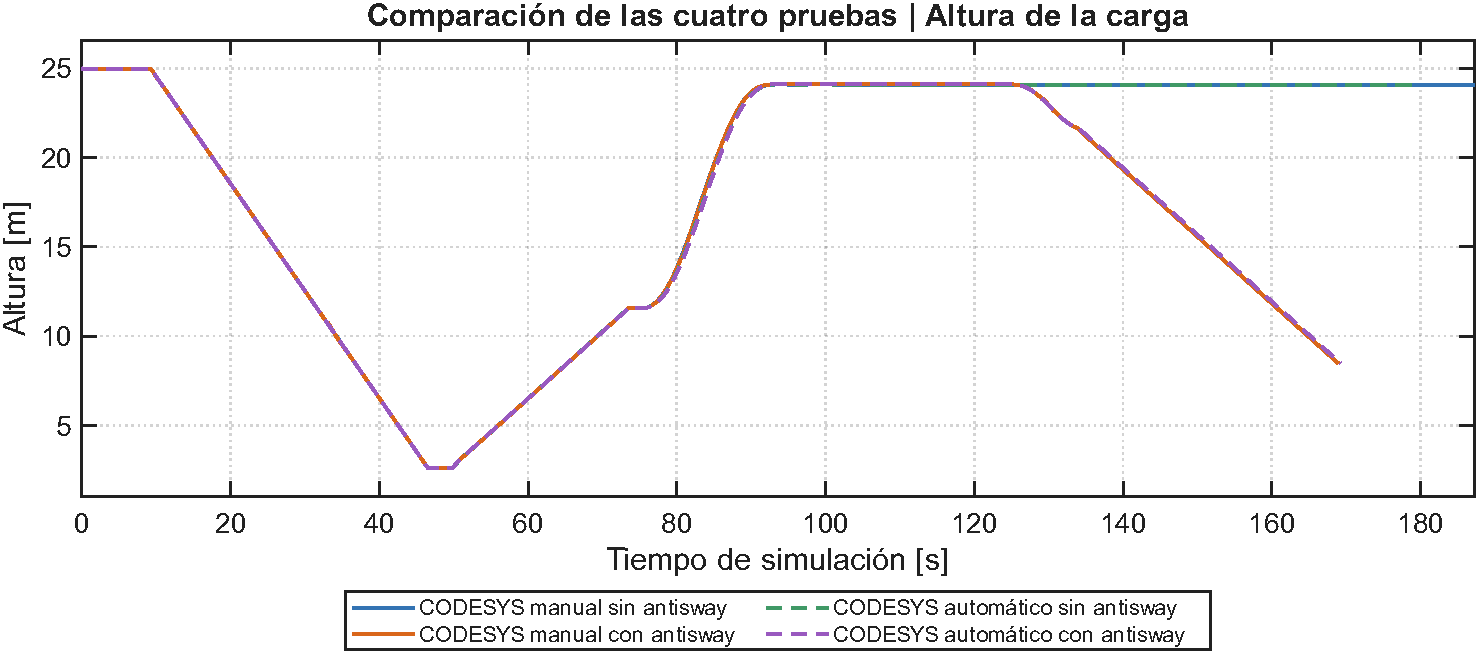
\includegraphics[width=0.98\textwidth]{graficas_individuales/comparacion_y.pdf}
\caption{Comparación de las cuatro pruebas: altura de la carga. Las curvas con antisway terminan en el apoyo o intento de entrega: 168,92 s para CODESYS manual y 169,24 s para CODESYS automático. Las variantes sin antisway conservan su duración y cobertura disponibles.}\label{fig:individual_comparacion_y}
\end{figure}

\begin{figure}[!htbp]
\centering
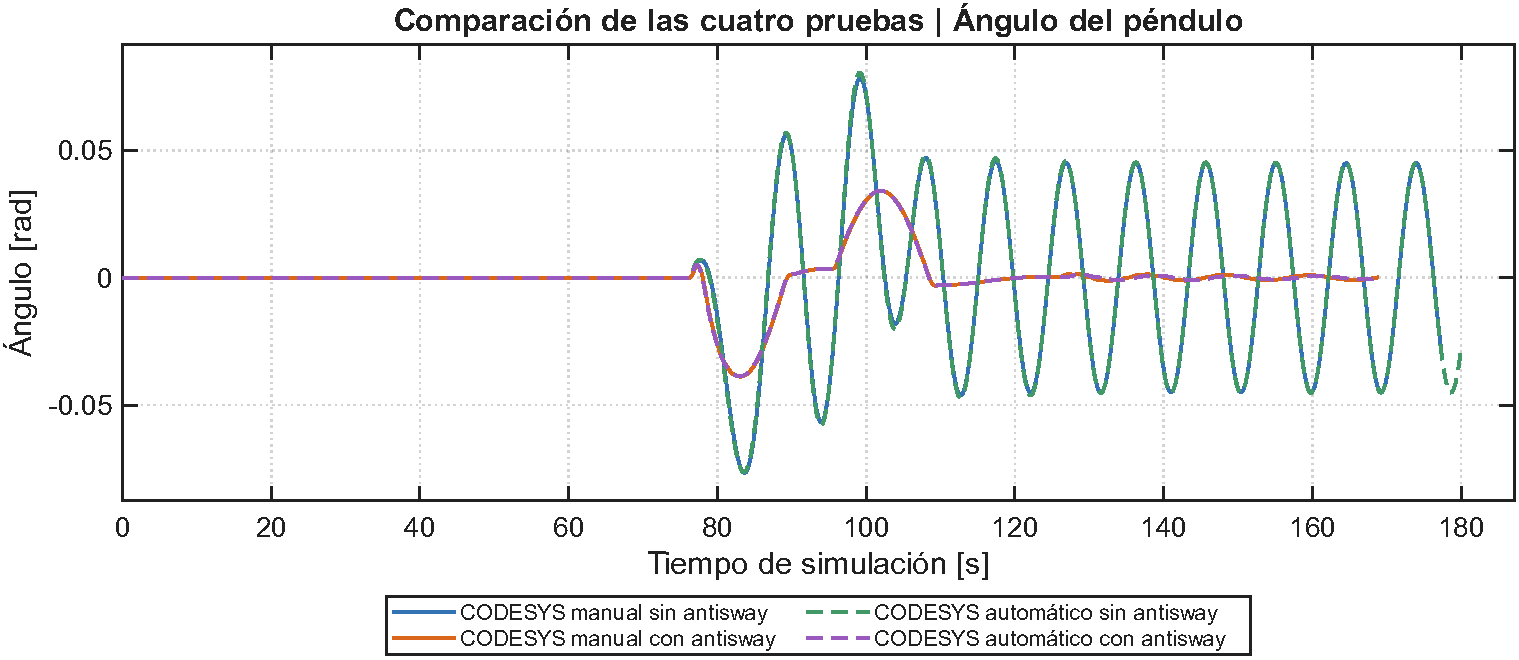
\includegraphics[width=0.98\textwidth]{graficas_individuales/comparacion_theta.pdf}
\caption{Comparación de las cuatro pruebas: ángulo del péndulo. Las curvas con antisway terminan en el apoyo o intento de entrega: 168,92 s para CODESYS manual y 169,24 s para CODESYS automático. Las variantes sin antisway conservan su duración y cobertura disponibles.}\label{fig:individual_comparacion_theta}
\end{figure}

\begin{figure}[!htbp]
\centering
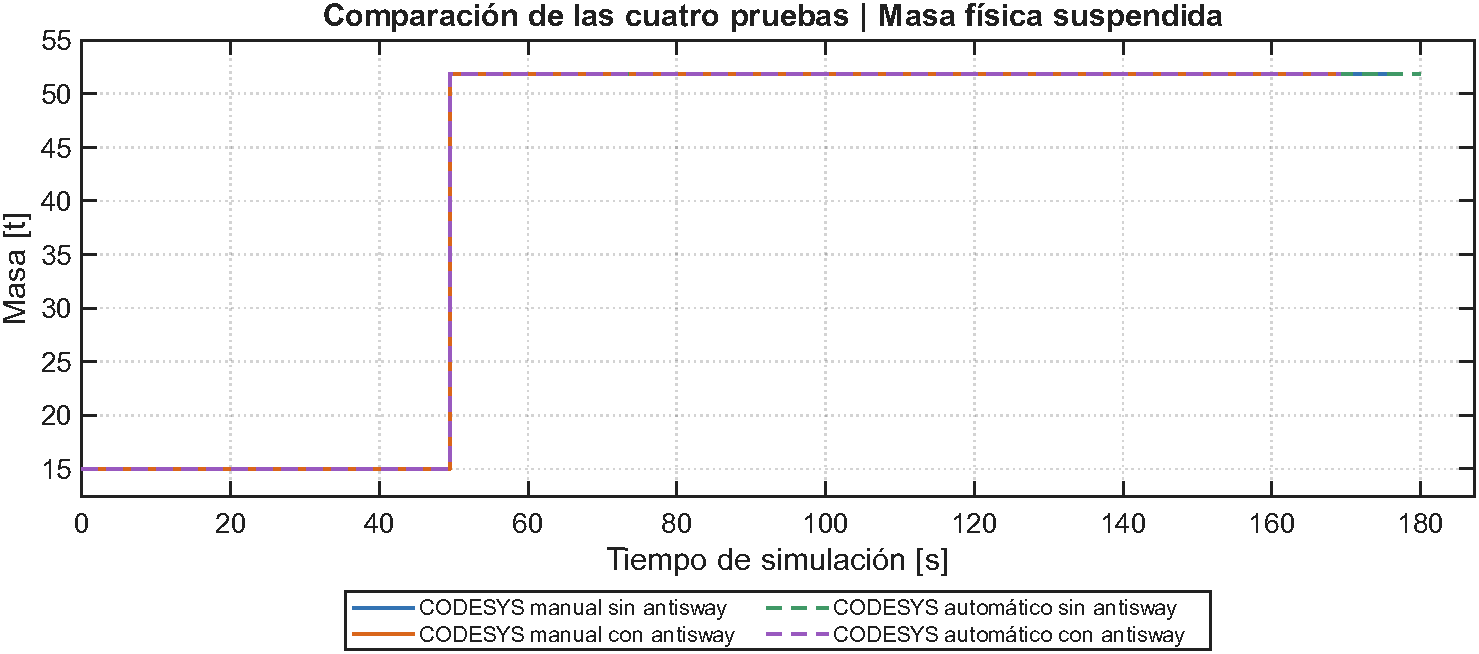
\includegraphics[width=0.98\textwidth]{graficas_individuales/comparacion_masa.pdf}
\caption{Comparación de las cuatro pruebas: masa física suspendida. Las curvas con antisway terminan en el apoyo o intento de entrega: 168,92 s para CODESYS manual y 169,24 s para CODESYS automático. Las variantes sin antisway conservan su duración y cobertura disponibles.}\label{fig:individual_comparacion_masa}
\end{figure}

\begin{figure}[!htbp]
\centering
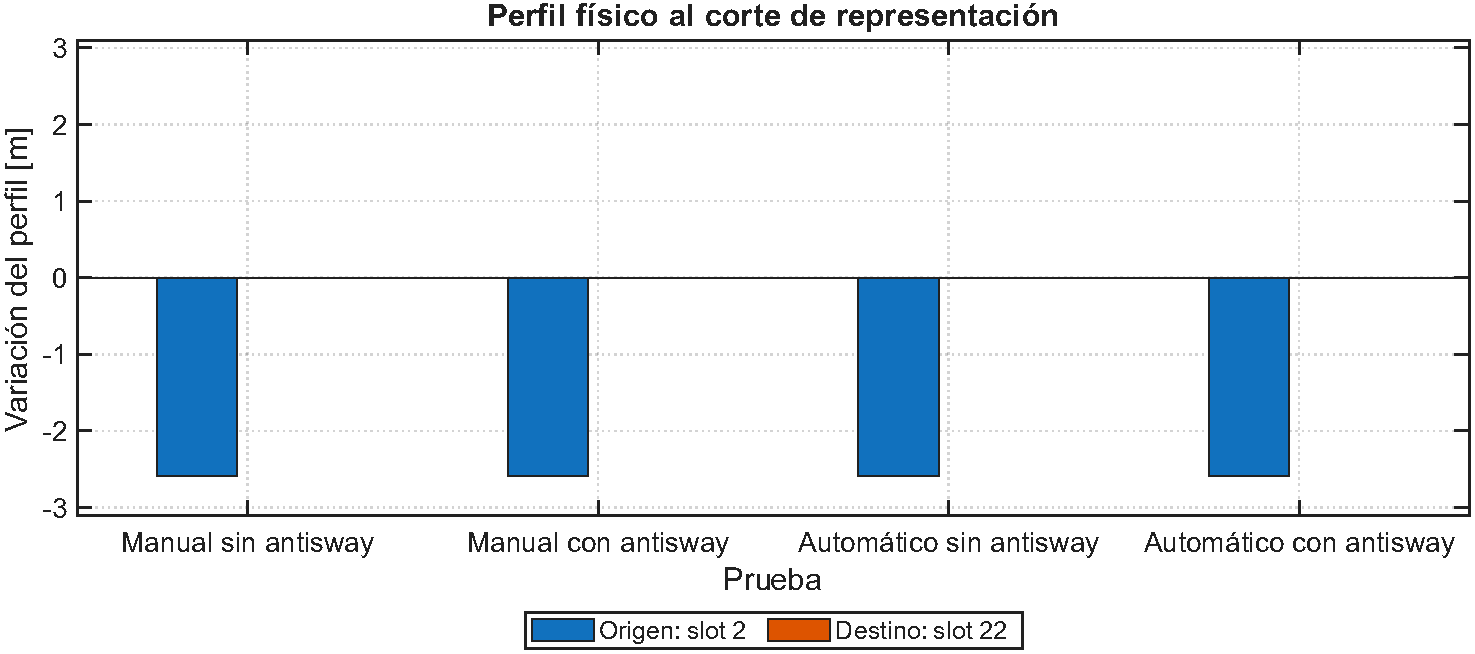
\includegraphics[width=0.98\textwidth]{graficas_individuales/perfil.pdf}
\caption{Variación del perfil físico hasta el final del intervalo graficado. Se observa el retiro en origen; el corte de las variantes con antisway se realiza antes de la confirmación de descarga. La entrega posterior de CODESYS manual con antisway se conserva como resultado del registro completo en el texto.}\label{fig:actual_perfil}
\end{figure}

\subsection{Seguridad observada y límites de interpretación}
Desde START hasta fin no se registraron fallas de PLC ni emergencias en las cuatro maniobras; las paradas incompletas no fueron abortos por fallo del PLC. La vigilancia de comunicación se mantiene independiente del reloj de la planta. Esta observación nominal no sustituye pruebas de emergencia, límites últimos, congelamiento del enlace o sobrevelocidad.

El margen geométrico mínimo aproximado en automático fue $2.658~\mathrm{m}$ para CODESYS manual con antisway, $2.626~\mathrm{m}$ para CODESYS automático sin antisway y $2.668~\mathrm{m}$ para CODESYS automático con antisway. Se calcula con huella rectangular y perfil físico, sin inclinación; el canal dedicado de colisión no estuvo disponible. Por ello no se certifica ausencia dinámica de colisiones. Se ocultó únicamente el mensaje de colisión de la HMI; no se anuló la lógica ni se convirtió un valor no disponible en cero.

\subsection{Cobertura y método de representación}
Los modos de funcionamiento se describen en el texto y no se grafican ni se marcan sobre los ejes. Cada figura contiene una sola gráfica. Por criterio de representación, todas las curvas temporales de CODESYS manual con antisway terminan en el apoyo a $168.92~\mathrm{s}$ y las de CODESYS automático con antisway en el intento de entrega a $169.24~\mathrm{s}$. Las dos variantes sin antisway conservan su duración completa, respetando su cobertura registrada. Los resultados finales de entrega y bloqueo se obtienen del registro completo posterior al corte, que permanece intacto; la masa graficada hasta el apoyo todavía incluye el contenedor. Las bandas grises muestran el intervalo previo a la toma confirmada y las bandas lavanda el tramo posterior a la llegada horizontal; las marcas corresponden a eventos físicos. La aceleración de izaje se presenta en escala completa y, por separado, con zoom vertical de $-1$ a $+1~\mathrm{m/s^2}$, sin alterar ni filtrar los datos. Las gráficas conservan los tiempos originales de las señales físicas, del controlador y de los torques. Las referencias, monitores y errores procesados se representan por tiempo sobre una rejilla de $40~\mathrm{ms}$, con interpolación para señales continuas y retención previa para estados discretos. Los tramos fuera de cobertura se excluyen. Se distinguen referencias, consignas y señales físicas, conservando los transitorios de contacto, elasticidad y arranque. La velocidad angular de referencia es una derivada numérica sobre la rejilla de análisis; la velocidad angular física es nativa.

CODESYS manual sin antisway sufrió interrupción de registro por almacenamiento: control y monitores hasta $130.72~\mathrm{s}$, numerosas señales físicas hasta $177.305~\mathrm{s}$, telemetría de operador hasta $187.20~\mathrm{s}$. Esta telemetría permite documentar la posición y el estado final, pero no recuperar el torque ni demostrar máximos nativos del tramo ausente. Las otras tres pruebas conservan registro nativo hasta la parada; las señales constantes de inicialización se identifican como constantes, sin exigirles una muestra final artificial.

Cada prueba conserva video de visualización y HMI. En CODESYS manual sin antisway, la captura cada $0.52~\mathrm{s}$ produce 180 s de reproducción para $187.20~\mathrm{s}$ simulados: prevalece el reloj de simulación. El retardo de redibujo impide utilizar la captura final como evidencia única de parada o descarga.
